\documentclass[11pt,a4paper]{report}

% ---------------------------------------------------------------------------
% Packages
% ---------------------------------------------------------------------------
\usepackage[margin=2.5cm]{geometry}
\usepackage[utf8]{inputenc}
\usepackage[T1]{fontenc}
\usepackage{graphicx}
\usepackage{xcolor}
\usepackage{booktabs}
\usepackage{enumitem}
\usepackage{parskip}
\usepackage{fancyhdr}
\usepackage{listings}
\usepackage{caption}
\usepackage{longtable}
\usepackage{amsmath}
\usepackage{array}
\usepackage[colorlinks=true,linkcolor=blue!55!black,citecolor=blue!55!black,
            urlcolor=blue!55!black]{hyperref}

% ---------------------------------------------------------------------------
% Listings style
% ---------------------------------------------------------------------------
\definecolor{codebg}{rgb}{0.96,0.96,0.96}
\definecolor{codekw}{rgb}{0.0,0.0,0.6}
\definecolor{codecomment}{rgb}{0.35,0.45,0.35}
\definecolor{codestr}{rgb}{0.6,0.1,0.1}

\lstset{
  basicstyle=\ttfamily\small,
  backgroundcolor=\color{codebg},
  keywordstyle=\color{codekw}\bfseries,
  commentstyle=\color{codecomment}\itshape,
  stringstyle=\color{codestr},
  showstringspaces=false,
  breaklines=true,
  breakatwhitespace=false,
  frame=single,
  rulecolor=\color{gray!40},
  xleftmargin=2pt,
  xrightmargin=2pt,
  framexleftmargin=6pt,
  framexrightmargin=6pt,
  tabsize=4,
  columns=fullflexible,
  language=Python,
}

% ---------------------------------------------------------------------------
% Header/footer
% ---------------------------------------------------------------------------
\pagestyle{fancy}
\fancyhf{}
\fancyhead[L]{\small\nouppercase{\leftmark}}
\fancyhead[R]{\small pySMOKEPostProcessor User Guide}
\fancyfoot[C]{\thepage}
\renewcommand{\headrulewidth}{0.4pt}

% ---------------------------------------------------------------------------
% Helper macros
% ---------------------------------------------------------------------------
\newcommand{\pyclass}[1]{\subsection{\texttt{#1}}}
\newcommand{\pyfunc}[1]{\subsubsection{\texttt{#1}}}
\newcommand{\pymethod}[1]{\subsubsection{\texttt{#1}}}
\newcommand{\returns}{\vspace{2mm}\noindent\textbf{Returns:} }
\newcommand{\raises}{\vspace{2mm}\noindent\textbf{Raises:} }
\newenvironment{params}{\vspace{1mm}\noindent\textbf{Parameters:}\begin{itemize}[leftmargin=1.1cm,label={--},itemsep=1pt,topsep=2pt]}{\end{itemize}}
\newcommand{\pkg}[1]{\lstinline|#1|}

\setcounter{secnumdepth}{3}
\setcounter{tocdepth}{2}

% ---------------------------------------------------------------------------
\title{\Huge \textbf{pySMOKEPostProcessor}\\[4mm]\Large User Guide}
\author{Documentation compiled for the \texttt{pySMOKEdev} repository}
\date{\today\ --- package version 0.3.0}

\begin{document}

\begin{titlepage}
\centering
\vspace*{3cm}
{\Huge\bfseries pySMOKEPostProcessor\par}
\vspace{0.5cm}
{\Large User Guide\par}
\vspace{1.5cm}
{\large Python post-processing toolkit for OpenSMOKE++:\\Rate-of-Production Analysis, Sensitivity Analysis, Elementary
Flux Analysis, reaction/formation rates, species- and reaction-class
analysis, and soot post-processing.\par}
\vspace{2cm}
{\large \today\par}
\vfill
%{\small Original computational core: OpenSMOKE++ Graphical Post Processor,
% Prof.\ Alberto Cuoci (Politecnico di Milano). Python/pybind11 wrapper:
% T.\ Dinelli, L.\ Pratali Maffei, E.\ Ramalli, A.\ Nobili, L.\ Giardini.\par}
\end{titlepage}

\tableofcontents
\clearpage

% =============================================================================
\part{Installation}
% =============================================================================

\chapter{Overview}

\texttt{pySMOKEPostProcessor} is a \emph{compiled} Python package: a
\href{https://github.com/pybind/pybind11}{pybind11} C++ extension module
providing the numerically heavy post-processing core, plus a pure-Python
layer on top providing the user-facing API, orchestration helpers and
plotting utilities. There is no pure-Python installation path --- the C++
extension must always be compiled against the OpenSMOKE++ headers.

The build is driven by \pkg{scikit-build-core} (a CMake-based PEP 517 build
backend), so from the user's point of view installation is still a single
\pkg{pip install} once the native prerequisites are available. Native
dependencies (Boost, Eigen3, the OpenSMOKE++ headers, pybind11) are resolved
automatically by the CMake configuration described in this chapter.

\chapter{Prerequisites}

\begin{itemize}
\item A C++14-capable compiler (GCC $\geq$ 9, Clang $\geq$ 10, or MSVC 2019+
  on Windows).
\item \href{https://docs.conda.io/}{conda} used for the native (non-Python) dependencies.
\item CMake $\geq$ 3.16.
\item Python $\geq$ 3.10.
\item Network access for the first build (to fetch OpenSMOKE++ headers and,
  if not already present, pybind11/Eigen3 via CMake \pkg{FetchContent}) ---
  or a local checkout of OpenSMOKE++, see Section~\ref{sec:opensmoke-headers}.
\end{itemize}

Platform-specific compiler setup:
\begin{description}[leftmargin=2.2cm]
\item[Linux (Debian/Ubuntu)] \pkg{sudo apt-get install build-essential}
\item[Linux (RHEL/CentOS)] \pkg{sudo yum groupinstall "Development Tools"}
\item[macOS] \pkg{xcode-select --install}
\item[Windows] Visual Studio 2019+ with the "Desktop development with C++"
  workload, or \pkg{conda install cxx-compiler}
\end{description}

\chapter{Quick installation}

\begin{lstlisting}[language=bash]
# 1. Clone the repository
git clone https://github.com/CRECKMODELING/pySMOKEPostProcessor.git
cd pySMOKEPostProcessor

# 2. Create and activate the conda environment (native deps: Boost, Eigen,
#    CMake, plus the Python runtime dependencies)
conda env create -f environment.yml
conda activate pp            # environment name as declared in environment.yml

# 3. Install the package
pip install .                  # end users
pip install -e .            # developers (editable install, recompiles
                            # the extension on every `pip install -e .`
                            # after a C++ change; Python-only changes are
                            # picked up immediately, no reinstall needed)
\end{lstlisting}

The first build actually takes a lot of times due to the large package. During \pkg{pip install}, the
build system (via \pkg{cmake/external/*.cmake}):
\begin{enumerate}
\item locates Boost ($\geq$ 1.70, \textbf{required}, not auto-fetched) and
  Eigen3 ($\geq$ 3.3, auto-fetched via CMake \pkg{FetchContent} if not found
  on the system/conda environment) from the active conda environment;
\item resolves the OpenSMOKE++ v0.24 headers (see below);
\item fetches pybind11 (via \pkg{FetchContent} if not already installed);
\item compiles \texttt{cxx\_wrapper/PostProcessorWrapper\_py.cpp} into the
  \pkg{pySMOKEPostProcessor.pySMOKEPostProcessor} extension module and
  installs it alongside the pure-Python package.
\end{enumerate}

For a verbose build (useful when diagnosing a failure):
\begin{lstlisting}[language=bash]
pip install . -vvv
\end{lstlisting}

\section{Resolving the OpenSMOKE++ headers}
\label{sec:opensmoke-headers}

The build needs the OpenSMOKE++ v0.24 sources (header-only library; nothing
is linked, only included). \pkg{cmake/external/OpenSMOKEpp.cmake} tries, in
order:

\begin{enumerate}
\item \textbf{\pkg{\$OpenSMOKEpp\_ROOT} environment variable} --- if set,
  \pkg{\$OpenSMOKEpp\_ROOT/source} is used directly. This is the recommended
  route for developers who already have a local OpenSMOKE++ checkout:
\begin{lstlisting}[language=bash]
export OpenSMOKEpp_ROOT=/path/to/OpenSMOKEpp
pip install -e .
\end{lstlisting}
\item \textbf{Vendored copy} --- \pkg{external/opensmoke/source} inside this
  repository, if present (not shipped by default).
\item \textbf{\pkg{FetchContent} from GitHub} --- clones
  \pkg{github.com/acuoci/OpenSMOKEpp} at tag \pkg{v0.24.0}. This repository is
  \textbf{private}; the clone needs credentials configured for the account
  running the build (SSH key or a git credential helper with access to the repository).
\end{enumerate}

If the build cannot find OpenSMOKE++, set \pkg{OpenSMOKEpp\_ROOT} to a local
checkout of the headers (option 1) rather than relying on the private-repo fetch.

\section{Manual CMake build}

\pkg{build/} is a standalone, git-ignored CMake tree that can be used instead
of \pkg{pip} to iterate purely on the C++ side:

\begin{lstlisting}[language=bash]
cmake -S . -B build
cmake --build build -j
\end{lstlisting}

This installs the compiled \pkg{.so}/\pkg{.pyd} directly into
\pkg{pySMOKEPostProcessor/}. \textbf{This is only meant for quick native
iteration}; the actual supported install path is always \pkg{pip install -e .},
which uses scikit-build-core's own editable-install machinery and correctly
places the extension inside the active environment's \pkg{site-packages}. Do
not mix the two: copying a manually-built \pkg{.so} into the source tree can
silently shadow the properly installed one.

\chapter{Verifying the installation}

\begin{lstlisting}[language=Python]
import pySMOKEPostProcessor
print("Installation successful!")
\end{lstlisting}

A more complete check is to run one of the bundled examples (example data
ships with the repository under \pkg{examples/data/}):

\begin{lstlisting}[language=bash]
cd examples/python
python RateOfProductionAnalysis_1.py
\end{lstlisting}

\chapter{Troubleshooting}

\begin{description}[leftmargin=3.2cm]
\item[CMake not found] \pkg{conda install cmake}
\item[Boost not found] \pkg{conda install boost-cpp}
\item[Eigen3 not found] normally auto-fetched; if that fails,
  \pkg{conda install eigen}
\item[OpenSMOKE++ fetch fails (git auth)] \pkg{conda install git} and ensure
  the account has access to the private OpenSMOKE++ repository, or set
  \pkg{OpenSMOKEpp\_ROOT} to a local checkout (Section~\ref{sec:opensmoke-headers}).
\item[Build fails with unclear errors] rebuild verbosely:
  \pkg{pip install . -vvv}, or force a clean build with
  \pkg{pip install . --no-build-isolation -v}
\end{description}

\chapter{Uninstalling}

\begin{lstlisting}[language=bash]
pip uninstall pySMOKEPostProcessor
conda deactivate
conda env remove -n pp
\end{lstlisting}

% =============================================================================
\part{User Guide}
% =============================================================================

\chapter{Overview}

The package is used almost entirely through one facade class,
\pkg{pySMOKEPostProcessor.PostProcessor}. It wraps a kinetic mechanism
(\pkg{kinetics.xml}, optionally with a coupled \pkg{kinetics.surface.xml})
and a simulation output (\pkg{Output.xml}) and exposes one method per
analysis (ROPA, sensitivity, flux, reaction classes, soot, \dots{}). Every
analysis method follows the same shape: it builds a fresh internal C++
"widget", pushes configuration through setters, runs the analysis, and
returns a plain Python \pkg{dict} (\pkg{"coefficients"}, \pkg{"reaction\_names"},
\pkg{"reaction\_indices"}) or a \pkg{pandas.DataFrame}. A small set of
standalone helper functions (\pkg{reaction\_classes.py}, \pkg{script\_utils.py})
then combine several \pkg{PostProcessor} analyses into higher-level workflows
(e.g.\ "reaction rates grouped by mechanism class, across many simulation
folders"), and the \pkg{plotting\_utilities} sub-package turns the resulting
dicts/DataFrames into matplotlib figures.

A minimal end-to-end example:

\begin{lstlisting}[language=Python]
from pySMOKEPostProcessor import PostProcessor
from pySMOKEPostProcessor.plotting_utilities.bar_plot import plot_bars

pp = PostProcessor(kineticFolder="path/to/kinetics",
                    outputFolder="path/to/Output")

ropa = pp.RateOfProductionAnalysis(species="H2", ropa_type="global",
                                    number_of_reactions=10)
# ropa == {"coefficients": [...], "reaction_names": [...], "reaction_indices": [...]}

fig, ax = plot_bars(ropa)
fig.show()
\end{lstlisting}

Types used throughout this guide: \pkg{str}, \pkg{int}, \pkg{float},
\pkg{bool}, \pkg{list}, \pkg{dict}, \pkg{pandas.DataFrame} and
\pkg{graphviz.Digraph} (an object with a \pkg{.render()} method and rich
Jupyter display support, e.g.\ via \pkg{IPython.display.display}).

\chapter{Quick reference}
\label{ch:quickref}

A one-page index of every public call covered in this part, for skimming.
Every entry links to its full description later in this part.

\section{\texttt{PostProcessor} (Chapters~3--9)}
\begin{center}
\small
\begin{longtable}{p{6.6cm}p{9cm}}
\toprule
\textbf{Call} & \textbf{Purpose} \\
\midrule
\endhead
\pkg{PostProcessor(kineticFolder, outputFolder, isHeterogeneous)} & construct; either input alone is enough for the methods that need only that one \\
\pkg{.updateOutput(outputFolder)} & re-point at a new \pkg{Output.xml}, same mechanism, no re-parse \\
\pkg{.getSpeciesProfile(name, basis, as\_dataframe)} & raw species mass/mole-fraction profile \\
\pkg{.getIndependentVariableProfile(as\_dataframe)} & time / spatial coordinate profile \\
\pkg{.getTemperatureProfile} / \pkg{.getPressureProfile} / \pkg{.getDensityProfile} / \pkg{.getViscosityProfile} / \pkg{.getYSootProfile} & raw \pkg{<additional>} column profiles \\
\pkg{.RateOfProductionAnalysis(species, ropa\_type, ..., heterogeneous\_reactions)} & ROPA, gas or (with \pkg{heterogeneous\_reactions=True}) surface ROPA on a mechanism \\
\pkg{.RateOfProductionAnalysis2D(species, ropa\_type, ...)} & ROPA for 2D/3D simulations \\
\pkg{.convert\_tomass(ropa\_coefficients, species)} & mole $\to$ mass unit conversion for a ROPA result \\
\pkg{.GetReactionRates(reaction\_name/reaction\_index, ...)} & full-profile reaction rate(s) \\
\pkg{.GetFormationRates(formation\_rate\_type, species, units, heterogeneous\_reactions)} & full-profile species formation rate \\
\pkg{.SensitivityAnalysis(target, sensitivity\_type, ...)} & sensitivity analysis, homogeneous mechanism \\
\pkg{.SensitivityAnalysis\_Surface(target, ...)} & sensitivity analysis, coupled gas+surface mechanism \\
\pkg{.SensitivityCoefficients(target, ...)} & \textit{time/coordinate evolution of the sensitivity coefficients} \\
\pkg{.FluxAnalysis(species, element, flux\_analysis\_type, ...)} & species-to-species element flux graph \\
\pkg{.ElementalDistributionByClass(element, normalize)} & element distribution across species classes \\
\pkg{.ElementMolesBySpecies(element)} & element distribution across individual species \\
\pkg{.FluxAnalysisByClass(element, flux\_analysis\_type, ...)} & class-to-class element flux matrix + graph \\
\pkg{.dfSootProperties} & attribute: full \pkg{<SootProperties>} BIN table \\
\pkg{.SootPSD(local\_value, particle\_type, diameter\_type, ...)} & soot particle size distribution \\
\pkg{.getFvSootProfile(as\_dataframe, min\_section)} & soot volume fraction $f_v$ along the abscissa \\
\pkg{.getSSASootProfile(as\_dataframe, min\_section)} & mean soot specific surface area along the abscissa \\
\pkg{.getHtoCSootProfile(as\_dataframe, min\_section, weighting)} & mean soot H/C along the abscissa \\
\bottomrule
\end{longtable}
\end{center}

\section{Module-level functions}
\begin{center}
\small
\begin{longtable}{p{6.6cm}p{9cm}}
\toprule
\textbf{Call} & \textbf{Purpose} \\
\midrule
\endhead
\pkg{reaction\_classes.merge\_maps\_byspecies(sorted\_dfs\_dct, ...)} & combine several simulations' class-flux tables \\
\pkg{reaction\_classes.FDI(sorted\_dfs\_dct, ...)} & Flux Diagnostic Index between simulations \\
\pkg{script\_utils.get\_sortedrxns(pp, class\_groups\_file, ...)} & classify a mechanism's reactions from its  \pkg{<ReactionClasses>} block \\
\pkg{script\_utils.process\_classes(...)} & multi-species ROPA grouped by reaction class \\
\pkg{script\_utils.cumulative\_rates(...)} & per-species cumulative rate tables \\
\pkg{script\_utils.reactionrates\_byclasses(...)} & time-resolved rates summed by reaction class \\
\pkg{plotting\_utilities.plot\_bars(data, ...)} & horizontal bar chart, ROPA/sensitivity dict \\
\pkg{plotting\_utilities.plot\_bars\_multiSimulation(data\_list, ...)} & grid of \pkg{plot\_bars} \\
\pkg{plotting\_utilities.plot\_heatmap(sort\_df, ...)} & diverging-colormap heatmap \\
\pkg{plotting\_utilities.plot\_class\_distribution(data\_df, ...)} & stacked-area, per-class distribution \\
\pkg{plotting\_utilities.plot\_areas(data\_df, ...)} & shaded-area / line plot, multi-column \pkg{DataFrame} \\
\pkg{plotting\_utilities.plot\_distribution(df, ...)} & soot PSD line plot \\
\pkg{elements\_balance(kineticFolder, resultsFolder, elements\_list, ...)} & element speciation stackplot \\
\pkg{surfacereactions\_utilities.CumulativeDeposition(...)} & cumulative surface-deposition stackplot \\
\pkg{surfacereactions\_utilities.CumulativeSootProduction(...)} & cumulative gas-phase soot stackplot \\
\bottomrule
\end{longtable}
\end{center}

\chapter{The \texttt{PostProcessor} facade}

\pyclass{PostProcessor}

The main entry point of the package. Every method in this chapter (unless
stated otherwise) is a method of this class.

\pymethod{PostProcessor(kineticFolder=None, outputFolder=None, isHeterogeneous=None)}

Constructs a post-processor around a mechanism and/or a simulation output.
Buildable from kinetics only, output only, or both --- calling a method that
needs an input that was not supplied raises a \pkg{RuntimeError}.

\begin{params}
\item \pkg{kineticFolder} (\textit{str}, optional) --- path to the folder
  containing \pkg{kinetics.xml} (and, if present, the coupled
  \pkg{kinetics.surface.xml}, autodetected).
\item \pkg{outputFolder} (\textit{str}, optional) --- path to the folder
  containing the simulation's \pkg{Output.xml}.
\item \pkg{isHeterogeneous} (\textit{bool}, optional) --- forces
  gas+surface handling. Only needed when constructing from
  \pkg{outputFolder} alone (no \pkg{kineticFolder}), since the
  heterogeneous/homogeneous distinction is otherwise auto-detected from the
  presence of \pkg{kinetics.surface.xml}.
\end{params}

\vspace{1mm}\noindent\textbf{Key attributes set on the instance:}
\begin{params}
\item \pkg{db} --- the underlying C++ \pkg{PostProcessorCore} orchestrator
  (owns both the kinetics and the output state; passed internally to every
  analysis widget).
\item \pkg{kineticFolder} / \pkg{outputFolder} --- last paths used.
\item \pkg{km} --- gas-phase kinetic map reader (\pkg{None} until a
  mechanism is loaded); exposes e.g.\ \pkg{speciesNames()},
  \pkg{reactionIndexFromName(name)}, \pkg{formattedReactionNameFromIndex(i)}.
\item \pkg{kmhet} --- the phase-2 kinetic map reader (surface, liquid or
  solid), if the mechanism has one, else \pkg{None}.
\item \pkg{isHeterogeneous} (\textit{bool}) --- \pkg{True} specifically when
  the loaded mechanism has a \emph{surface} phase-2 (a liquid/solid phase-2
  leaves this \pkg{False}); \pkg{SensitivityAnalysis\_Surface} branches on
  this flag internally, and it is otherwise a convenient guard for user code
  deciding whether to pass \pkg{heterogeneous\_reactions=True} to ROPA
  methods.
\item \pkg{soot} --- C++ \pkg{Soot} widget, always present once both
  kinetics and output are loaded; \pkg{soot.sootAvailable()} tells whether
  the mechanism actually has a \pkg{<SootProperties>} block.
\item \pkg{dfSootProperties} --- one-row-per-BIN \pkg{DataFrame} view of the
  whole \pkg{<SootProperties>} block (columns match OpenSMOKE's
  \pkg{BinProperties.txt}), or \pkg{None} if the mechanism has no soot BINs.
\end{params}

\pymethod{updateOutput(outputFolder: str) -> None}

Re-points this \pkg{PostProcessor} at a different \pkg{Output.xml} under the
\emph{same} mechanism, without re-parsing \pkg{kinetics.xml}. Intended for
the common "one mechanism, many output folders" pattern (parameter sweeps,
per-timestep re-analysis): build once, call \pkg{updateOutput} in a loop.
Requires an output to already be loaded (via \pkg{outputFolder} at
construction, or a previous successful \pkg{updateOutput} call).

\begin{params}
\item \pkg{outputFolder} (\textit{str}) --- path to the new output folder.
\end{params}

\chapter{Reading raw profiles}

These methods read directly from \pkg{Output.xml}, independent of the
kinetic mechanism.

\pymethod{getSpeciesProfile(name, basis="mass", as\_dataframe=False)}

\begin{params}
\item \pkg{name} (\textit{str}) --- species name.
\item \pkg{basis} (\textit{str}) --- \pkg{"mass"} or \pkg{"mole"}.
\item \pkg{as\_dataframe} (\textit{bool}) --- if \pkg{True}, return a
  single-column \pkg{DataFrame} indexed by the independent variable instead
  of a tuple.
\end{params}
\returns \pkg{(x, y)} as \pkg{numpy.ndarray} pairs (independent variable,
species profile), or a one-column \pkg{DataFrame} if \pkg{as\_dataframe=True}.

\pymethod{getIndependentVariableProfile(as\_dataframe=False)}

The independent variable is time for batch reactor, length for a flame, and either time or axial coordinate for plug flow reactor, based on the simulation setup ---
whichever OpenSMOKE++ wrote as the abscissa of \pkg{Output.xml}.
\returns \pkg{numpy.ndarray}, or a one-column \pkg{DataFrame} if
\pkg{as\_dataframe=True}.

\pymethod{getTemperatureProfile / getPressureProfile / getDensityProfile \\/ getViscosityProfile / getYSootProfile(as\_dataframe=False)}

Five near-identical getters for standard \pkg{<additional>} columns of
\pkg{Output.xml} (temperature, pressure, density, viscosity, soot mass
fraction --- the last one is legacy: no current solver writes it). Same
\pkg{as\_dataframe} flag as above.
\returns \pkg{(x, y)} tuple of \pkg{numpy.ndarray}, or a \pkg{DataFrame}.

Soot volume fraction is \emph{not} a raw \pkg{<additional>} column --- it is
a computed, mass-weighted average over BINs, documented with the other soot
getters in Chapter 9 (\pkg{getFvSootProfile}).

\chapter{Rate of Production Analysis (ROPA)}

\pymethod{RateOfProductionAnalysis(species, ropa\_type, local\_value=0, lower\_value=0, upper\_value=0, number\_of\_reactions=10, two\_dimensions=False, region\_location=None, mass\_ropa=False, include\_names=True) -> dict}

Performs a Rate Of Production Analysis for a gas-phase (homogeneous)
mechanism.

\begin{params}
\item \pkg{species} (\textit{str}) --- target species name.
\item \pkg{ropa\_type} (\textit{str}) --- \pkg{"global"}, \pkg{"local"} or
  \pkg{"region"}.
\item \pkg{local\_value} (\textit{float}) --- abscissa at which to evaluate,
  used when \pkg{ropa\_type="local"}.
\item \pkg{lower\_value} / \pkg{upper\_value} (\textit{float}) --- bounds of
  the integration region, used when \pkg{ropa\_type="region"}.
\item \pkg{number\_of\_reactions} (\textit{int}) --- number of reactions to
  keep in the result (ranked by contribution).
\item \pkg{two\_dimensions} (\textit{bool}) --- for 2D/3D simulations;
  delegates to \pkg{RateOfProductionAnalysis2D} (see below) when \pkg{True}.
\item \pkg{region\_location} (\textit{dict}) --- 2D-mode region definition,
  only used with \pkg{two\_dimensions=True}.
\item \pkg{mass\_ropa} (\textit{bool}) --- return coefficients in mass units
  instead of mole units (via \pkg{convert\_tomass}).
\item \pkg{include\_names} (\textit{bool}) --- resolve reaction names (one
  lookup per returned reaction). Callers that only need indices/coefficients
  can set this \pkg{False} to skip the (cheap, but non-zero over large
  species $\times$ timestep loops) name resolution.
\item \pkg{heterogeneous\_reactions} (\textit{bool}) --- run the ROPA on the
  surface reaction set instead of the gas one, for a coupled gas+surface
  mechanism (requires \pkg{pp.isHeterogeneous}); not supported together with
  \pkg{two\_dimensions=True}, and \pkg{mass\_ropa} is not supported together
  with this.
\end{params}
\returns \pkg{dict} with keys \pkg{"coefficients"} (\textit{list[float]}),
\pkg{"reaction\_names"} (\textit{list[str]}, or \pkg{None} if
\pkg{include\_names=False}), \pkg{"reaction\_indices"} (\textit{list[int]}).

\begin{figure}[h]
\centering
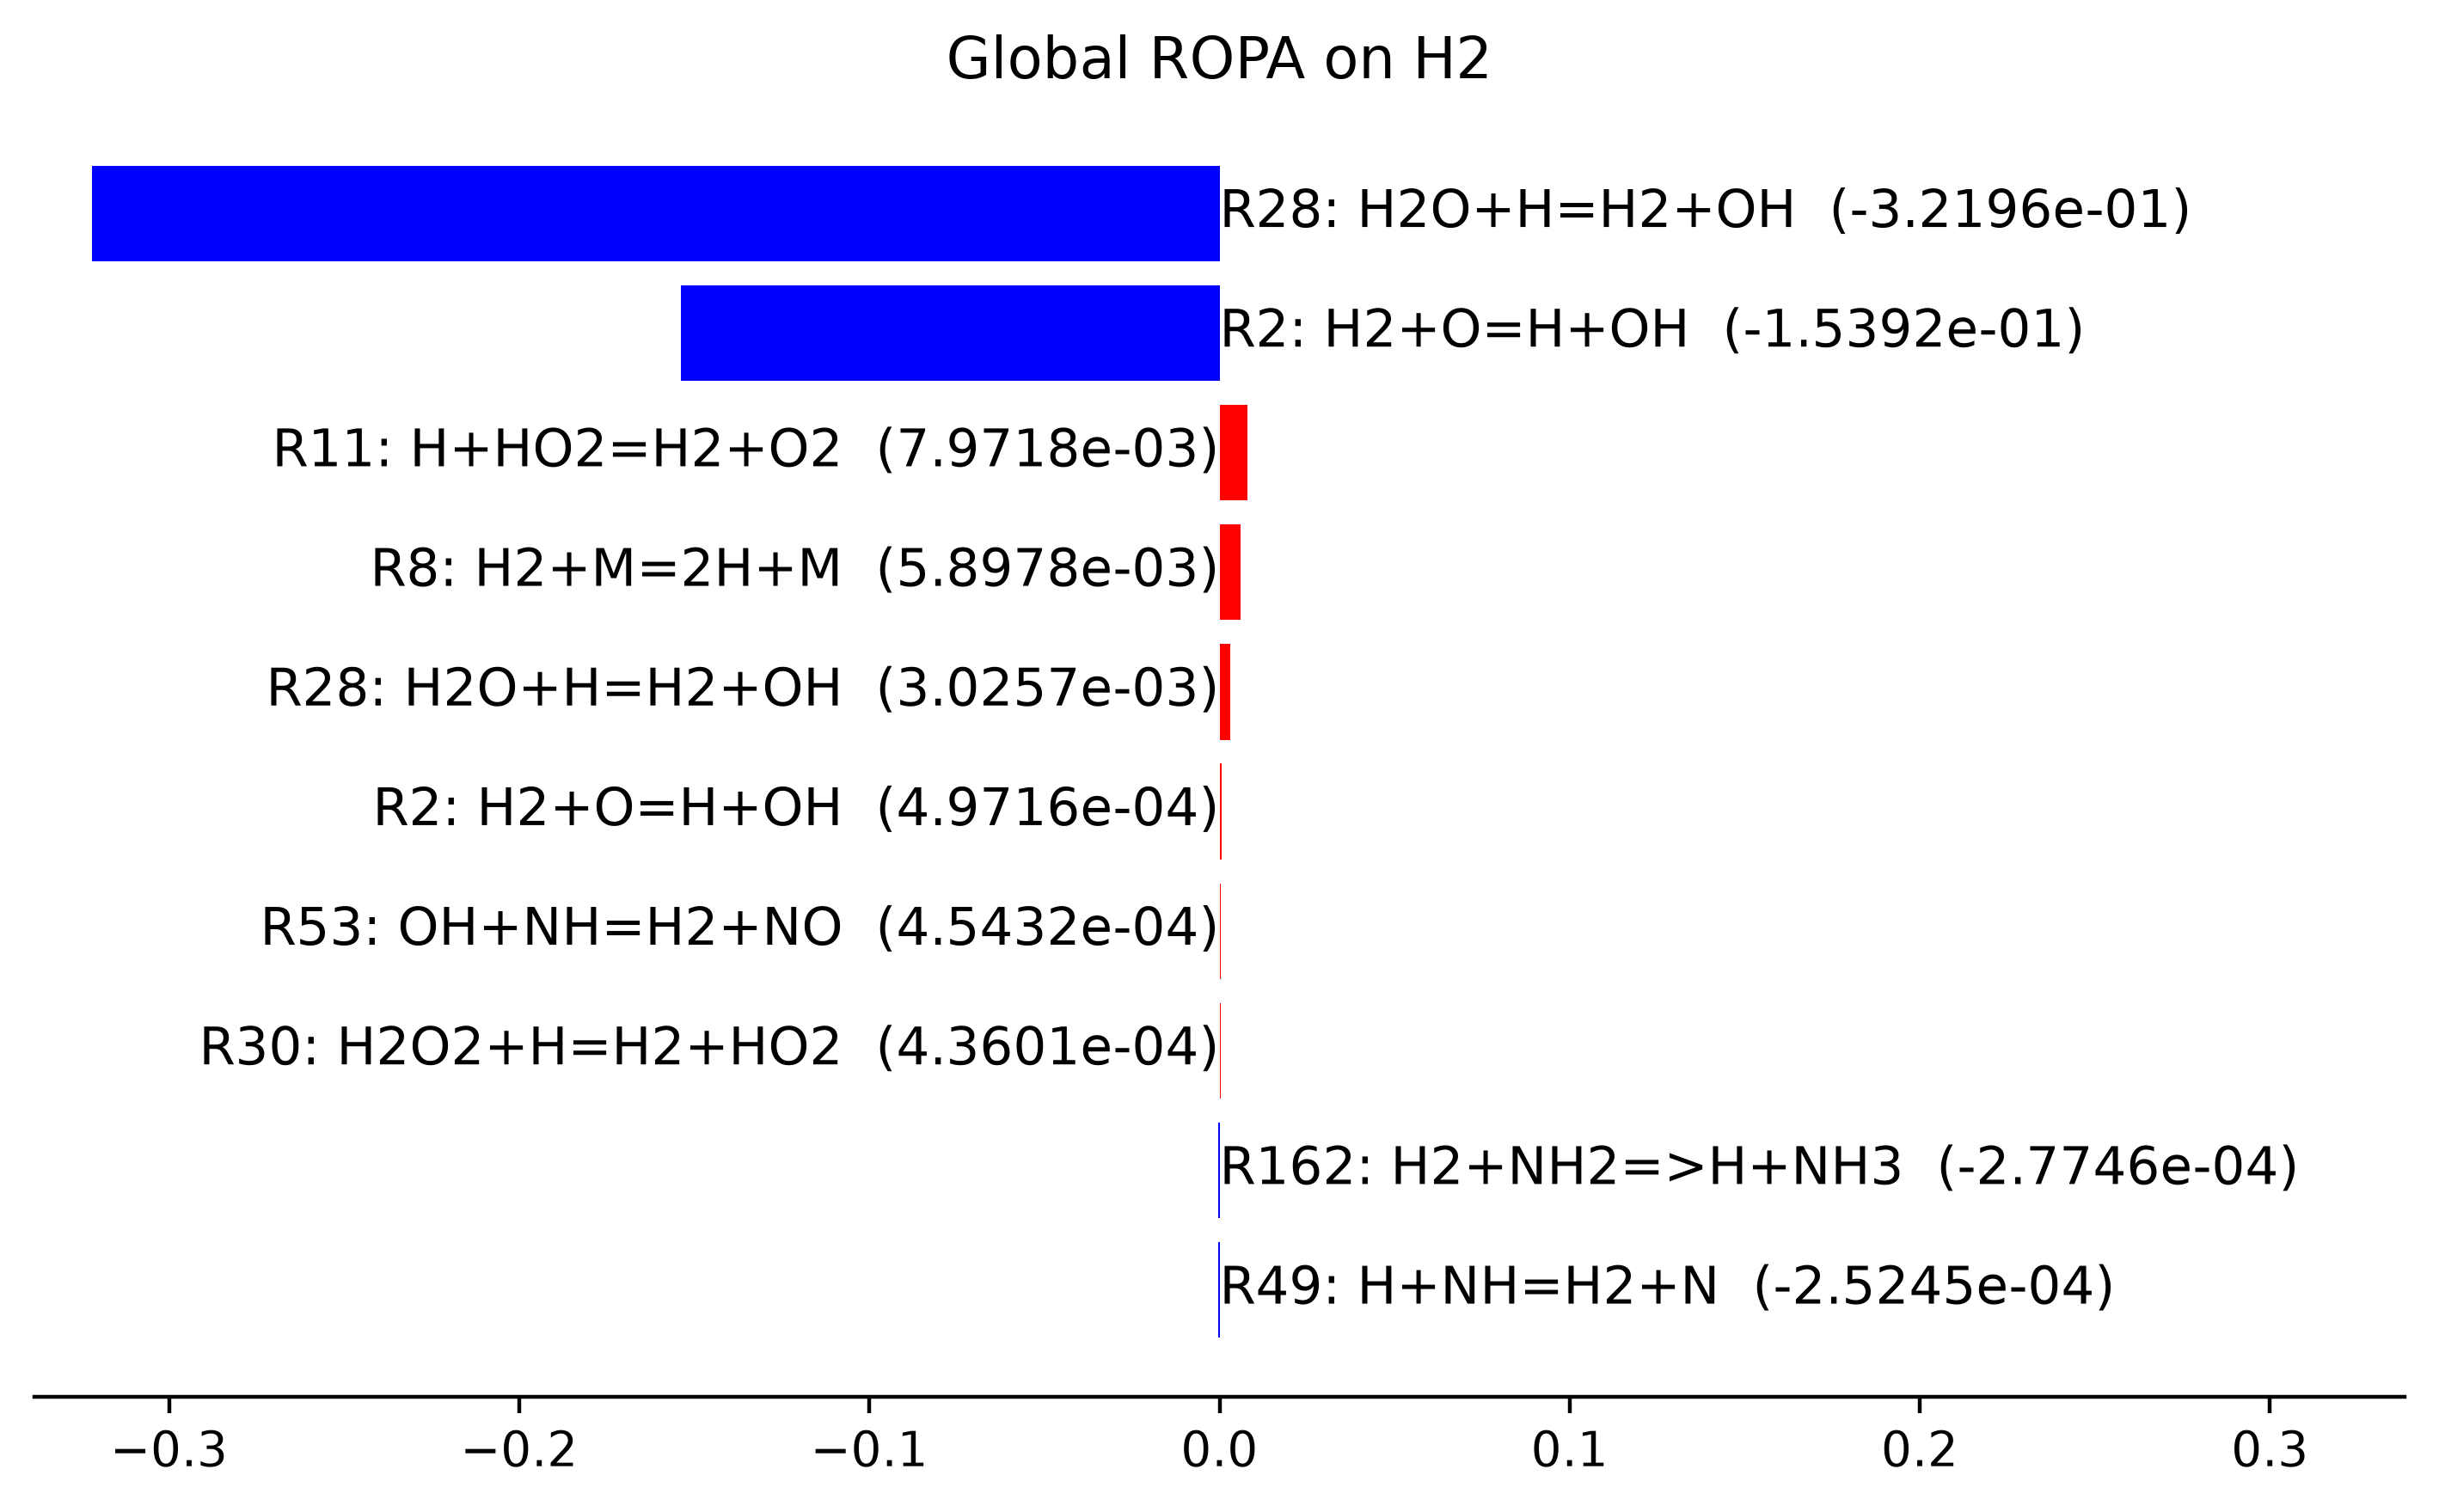
\includegraphics[width=0.75\textwidth]{figures/ropa_bars.png}
\caption{Global ROPA on H2, plotted with \texttt{plot\_bars} (Chapter~\ref{ch:plotting}). Red bars are production, blue bars are consumption.}
\end{figure}

The same call with \pkg{ropa\_type="local"} freezes the ROPA at one point of
the independent variable (the first point whose abscissa $\geq$
\pkg{local\_value}), while \pkg{ropa\_type="region"} integrates the
production/consumption rates between \pkg{lower\_value} and
\pkg{upper\_value} before ranking reactions --- useful when the "important"
reactions change quickly with time/space and a single \pkg{local} snapshot
would be noisy or misleading:

\begin{lstlisting}[language=Python]
local_ropa = pp.RateOfProductionAnalysis(species="H2", ropa_type="local",
                                          local_value=0.001, number_of_reactions=10)
region_ropa = pp.RateOfProductionAnalysis(species="H2", ropa_type="region",
                                           lower_value=0.0005, upper_value=0.0009,
                                           number_of_reactions=10)
\end{lstlisting}

\begin{figure}[h]
\centering
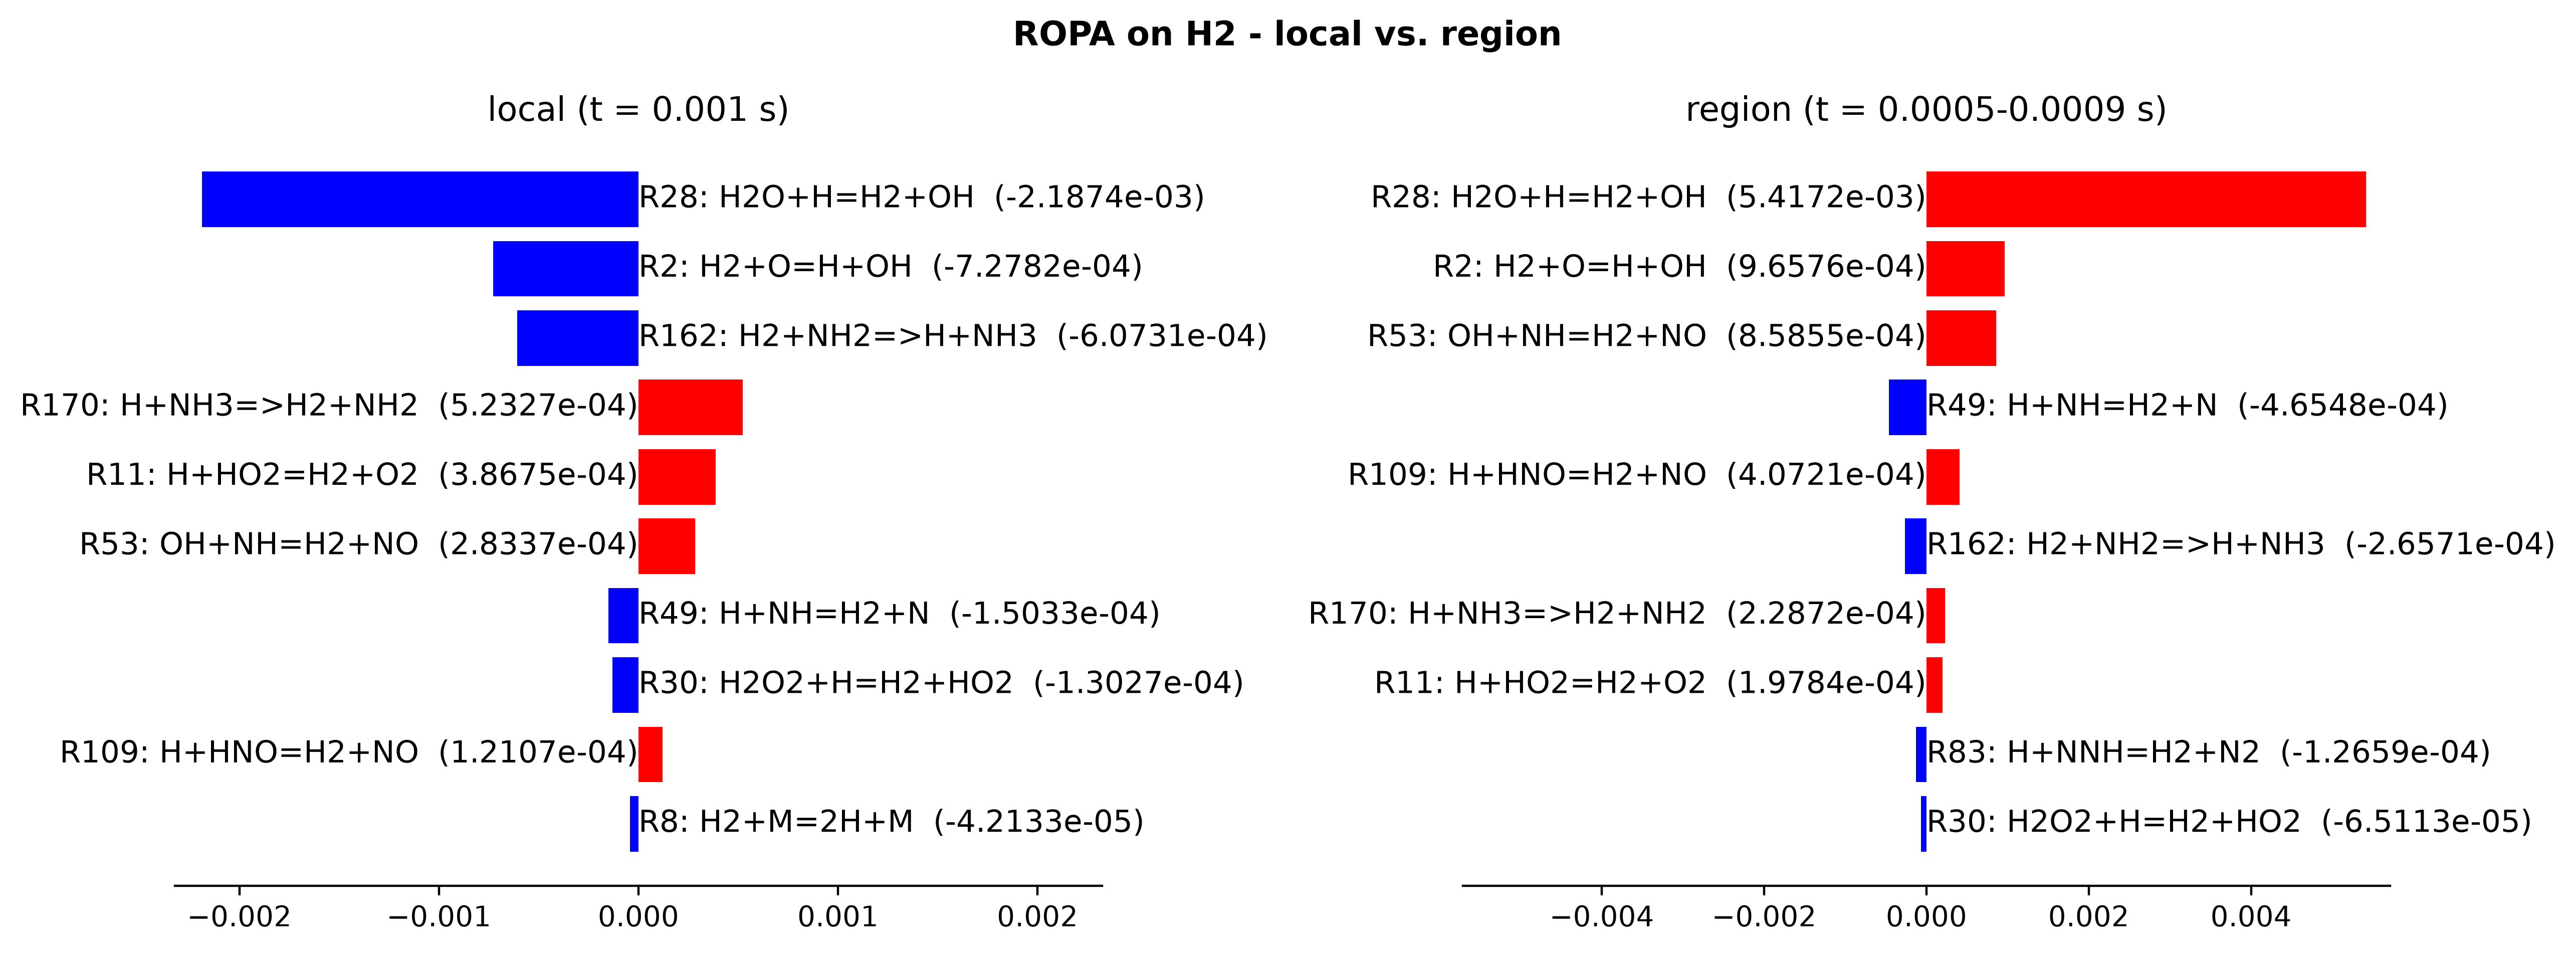
\includegraphics[width=0.95\textwidth]{figures/ropa_local_region.png}
\caption{The same H2 ROPA evaluated \texttt{local} at $t=0.001$\,s (left) vs.\ integrated over the \texttt{region} $t \in [0.0005, 0.0009]$\,s (right); note both the reaction set and the relative weights shift.}
\end{figure}

A coupled gas+surface (deposition) mechanism uses this same method with
\pkg{heterogeneous\_reactions=True} to run the ROPA on the surface reaction
set instead of a separate \pkg{\_Surface} call:

\begin{lstlisting}[language=Python]
gas_ropa = pp.RateOfProductionAnalysis("CH4", ropa_type="global",
                                        heterogeneous_reactions=False)
surf_ropa = pp.RateOfProductionAnalysis("C(B)", ropa_type="global",
                                         heterogeneous_reactions=True)
\end{lstlisting}

\pymethod{RateOfProductionAnalysis2D(species, ropa\_type, number\_of\_reactions=10, \\region\_location=None, mass\_ropa=False) -> dict}

The 2D/3D-simulation variant, normally reached through
\pkg{RateOfProductionAnalysis(..., two\_dimensions=True, region\_location=\{...\})}
rather than called directly.

\begin{params}
\item \pkg{region\_location} (\textit{dict}) --- must contain the six keys
  \pkg{local\_value\_x}, \pkg{local\_value\_z}, \pkg{lower\_value\_x},
  \pkg{lower\_value\_z}, \pkg{upper\_value\_x}, \pkg{upper\_value\_z}.
\end{params}
\returns same \pkg{dict} shape as \pkg{RateOfProductionAnalysis}.

\pymethod{convert\_tomass(ropa\_coefficients, species) -> list}

Converts ROPA coefficients from mole to mass units (multiplies by the
species' molecular weight).

\begin{params}
\item \pkg{ropa\_coefficients} (\textit{list[float]}) --- coefficients in
  mole units.
\item \pkg{species} (\textit{str}) --- species name (used to look up the
  molecular weight).
\end{params}
\returns \textit{list[float]}, coefficients in mass units.

\pymethod{GetReactionRates(reaction\_name=None, reaction\_index=None, sum\_rates=False, heterogeneous\_reactions=False) -> list}

Returns full time/coordinate profiles of one or more reaction rates (not
just a ROPA snapshot).

\begin{params}
\item \pkg{reaction\_name} (\textit{list[str]}, optional) --- reaction names;
  resolved to indices internally (mutually exclusive in practice with
  passing \pkg{reaction\_index} directly, though both parameters exist on
  the signature).
\item \pkg{reaction\_index} (\textit{list[int]}, optional) --- reaction
  indices.
\item \pkg{sum\_rates} (\textit{bool}) --- if \pkg{True}, sum all requested
  reactions into a single profile.
\item \pkg{heterogeneous\_reactions} (\textit{bool}) --- for coupled
  mechanisms, whether the given indices/names refer to the surface phase.
\end{params}
\returns \textit{list[list[float]]} (one profile per requested reaction), or
a one-element list containing the summed profile if \pkg{sum\_rates=True}.
Unlike \pkg{RateOfProductionAnalysis}, this is not a ranked snapshot: it is
the full profile of each named/indexed reaction, meant to be plotted against
the independent variable directly.

\begin{lstlisting}[language=Python]
_, temperature = pp.getTemperatureProfile()
names = ["O2+H=O+OH", "H2+O=H+OH", "O2+H(+M)=HO2(+M)"]
rates = pp.GetReactionRates(reaction_name=names)

for r, name in zip(rates, names):
    ax.plot(temperature, r, label=name)
\end{lstlisting}

\begin{figure}[h]
\centering
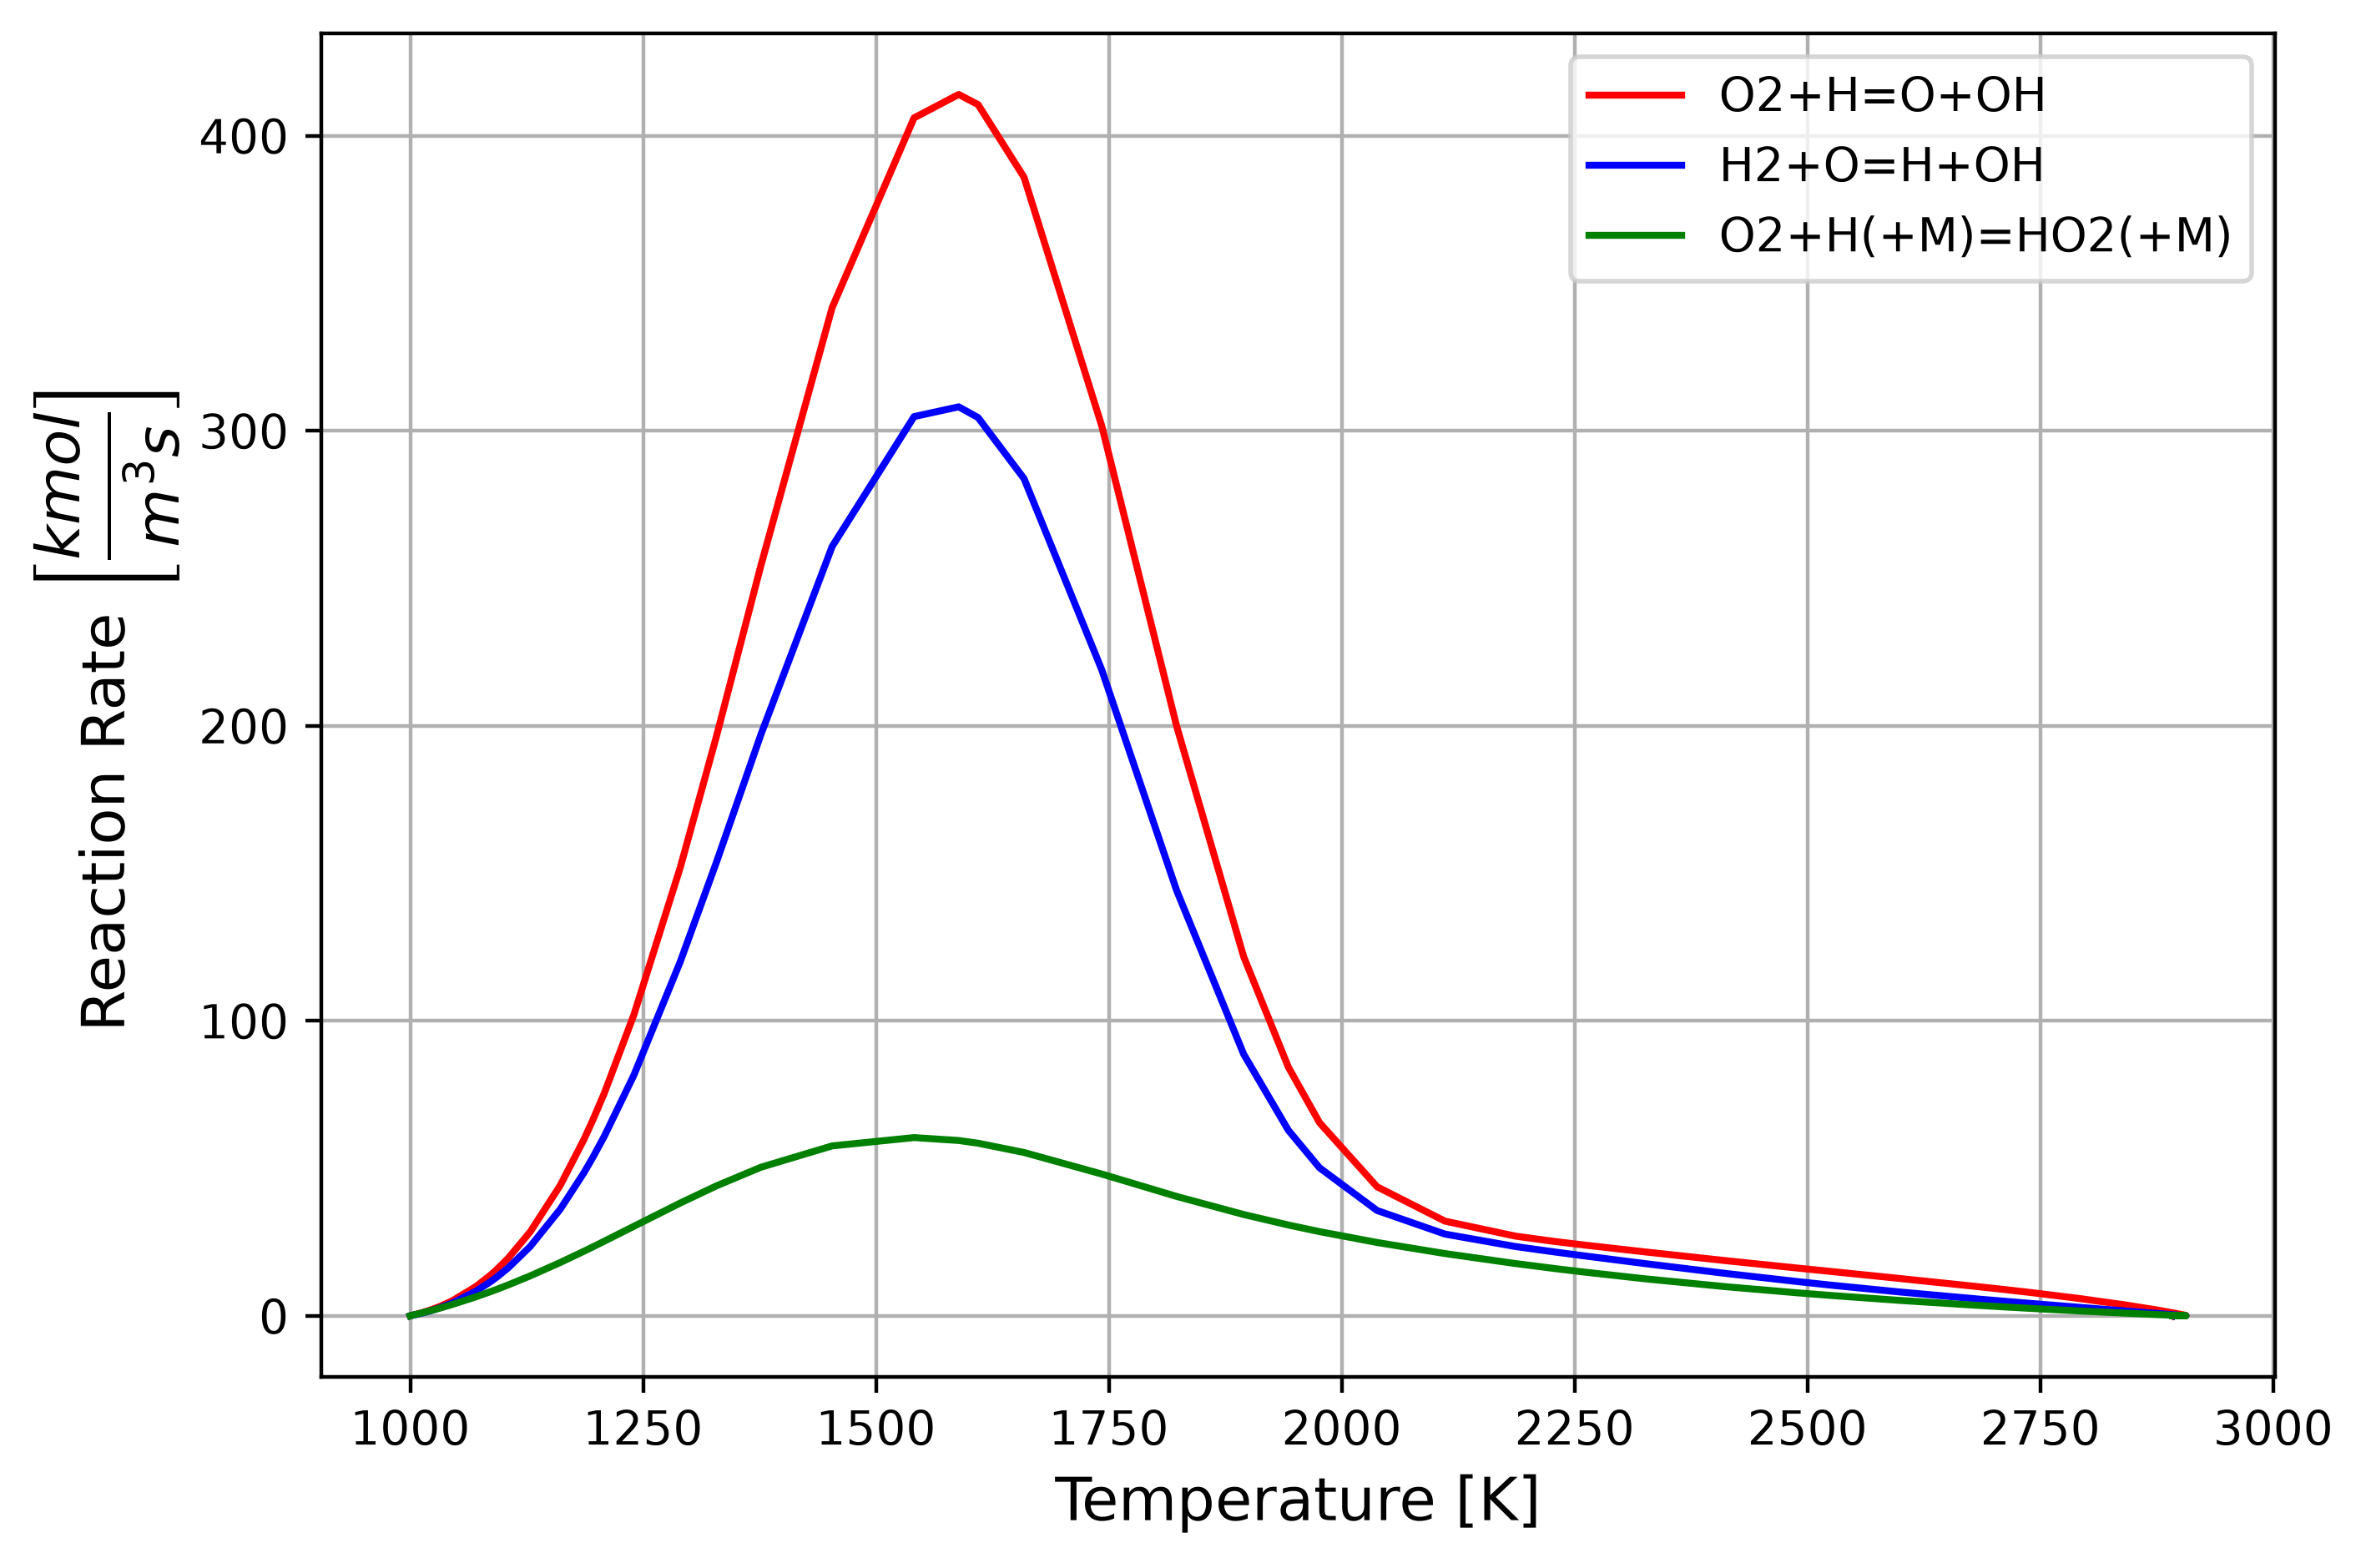
\includegraphics[width=0.75\textwidth]{figures/reaction_rates_lines.png}
\caption{Three reaction-rate profiles vs.\ temperature, from \texttt{GetReactionRates} plotted with plain matplotlib (no dedicated plotting helper is needed for a simple profile line plot).}
\end{figure}

\pymethod{GetFormationRates(formation\_rate\_type, species, units="mole", \\ heterogeneous\_reactions=False) -> list}

Formation-rate profile of a single species (all reactions combined).

\begin{params}
\item \pkg{formation\_rate\_type} (\textit{str}) --- formation-rate type as
  understood by the underlying \pkg{ROPA} widget.
\item \pkg{species} (\textit{str}) --- species name.
\item \pkg{units} (\textit{str}) --- \pkg{"mole"} (default) or \pkg{"mass"}.
\item \pkg{heterogeneous\_reactions} (\textit{bool}) --- formation rate from
  the surface reaction set instead of the gas one, for a coupled
  gas+surface mechanism.
\end{params}
\returns \textit{list[float]}, the formation-rate profile.

\chapter{Sensitivity Analysis}

\pymethod{SensitivityAnalysis(target, sensitivity\_type, ordering\_type="peak-values", normalization\_type="max-value", local\_value=0, lower\_value=0, upper\_value=0, number\_of\_reactions=10) -> dict}

\begin{params}
\item \pkg{target} (\textit{str}) --- target species for the sensitivity
  analysis.
\item \pkg{sensitivity\_type} (\textit{str}) --- e.g.\ \pkg{"global"},
  \pkg{"local"} (mechanism-dependent set of supported values).
\item \pkg{ordering\_type} (\textit{str}) --- how the returned reactions are
  ranked, e.g.\ \pkg{"peak-values"}.
\item \pkg{normalization\_type} (\textit{str}) --- e.g.\ \pkg{"max-value"},
  \pkg{"local"}.
\item \pkg{local\_value}, \pkg{lower\_value}, \pkg{upper\_value}
  (\textit{float}) --- same meaning as in ROPA.
\item \pkg{number\_of\_reactions} (\textit{int}) --- number of reactions to
  keep.
\end{params}
\returns \pkg{dict} with \pkg{"coefficients"}, \pkg{"reaction\_names"},
\pkg{"reaction\_indices"} (same shape as ROPA's result).

\begin{figure}[h]
\centering
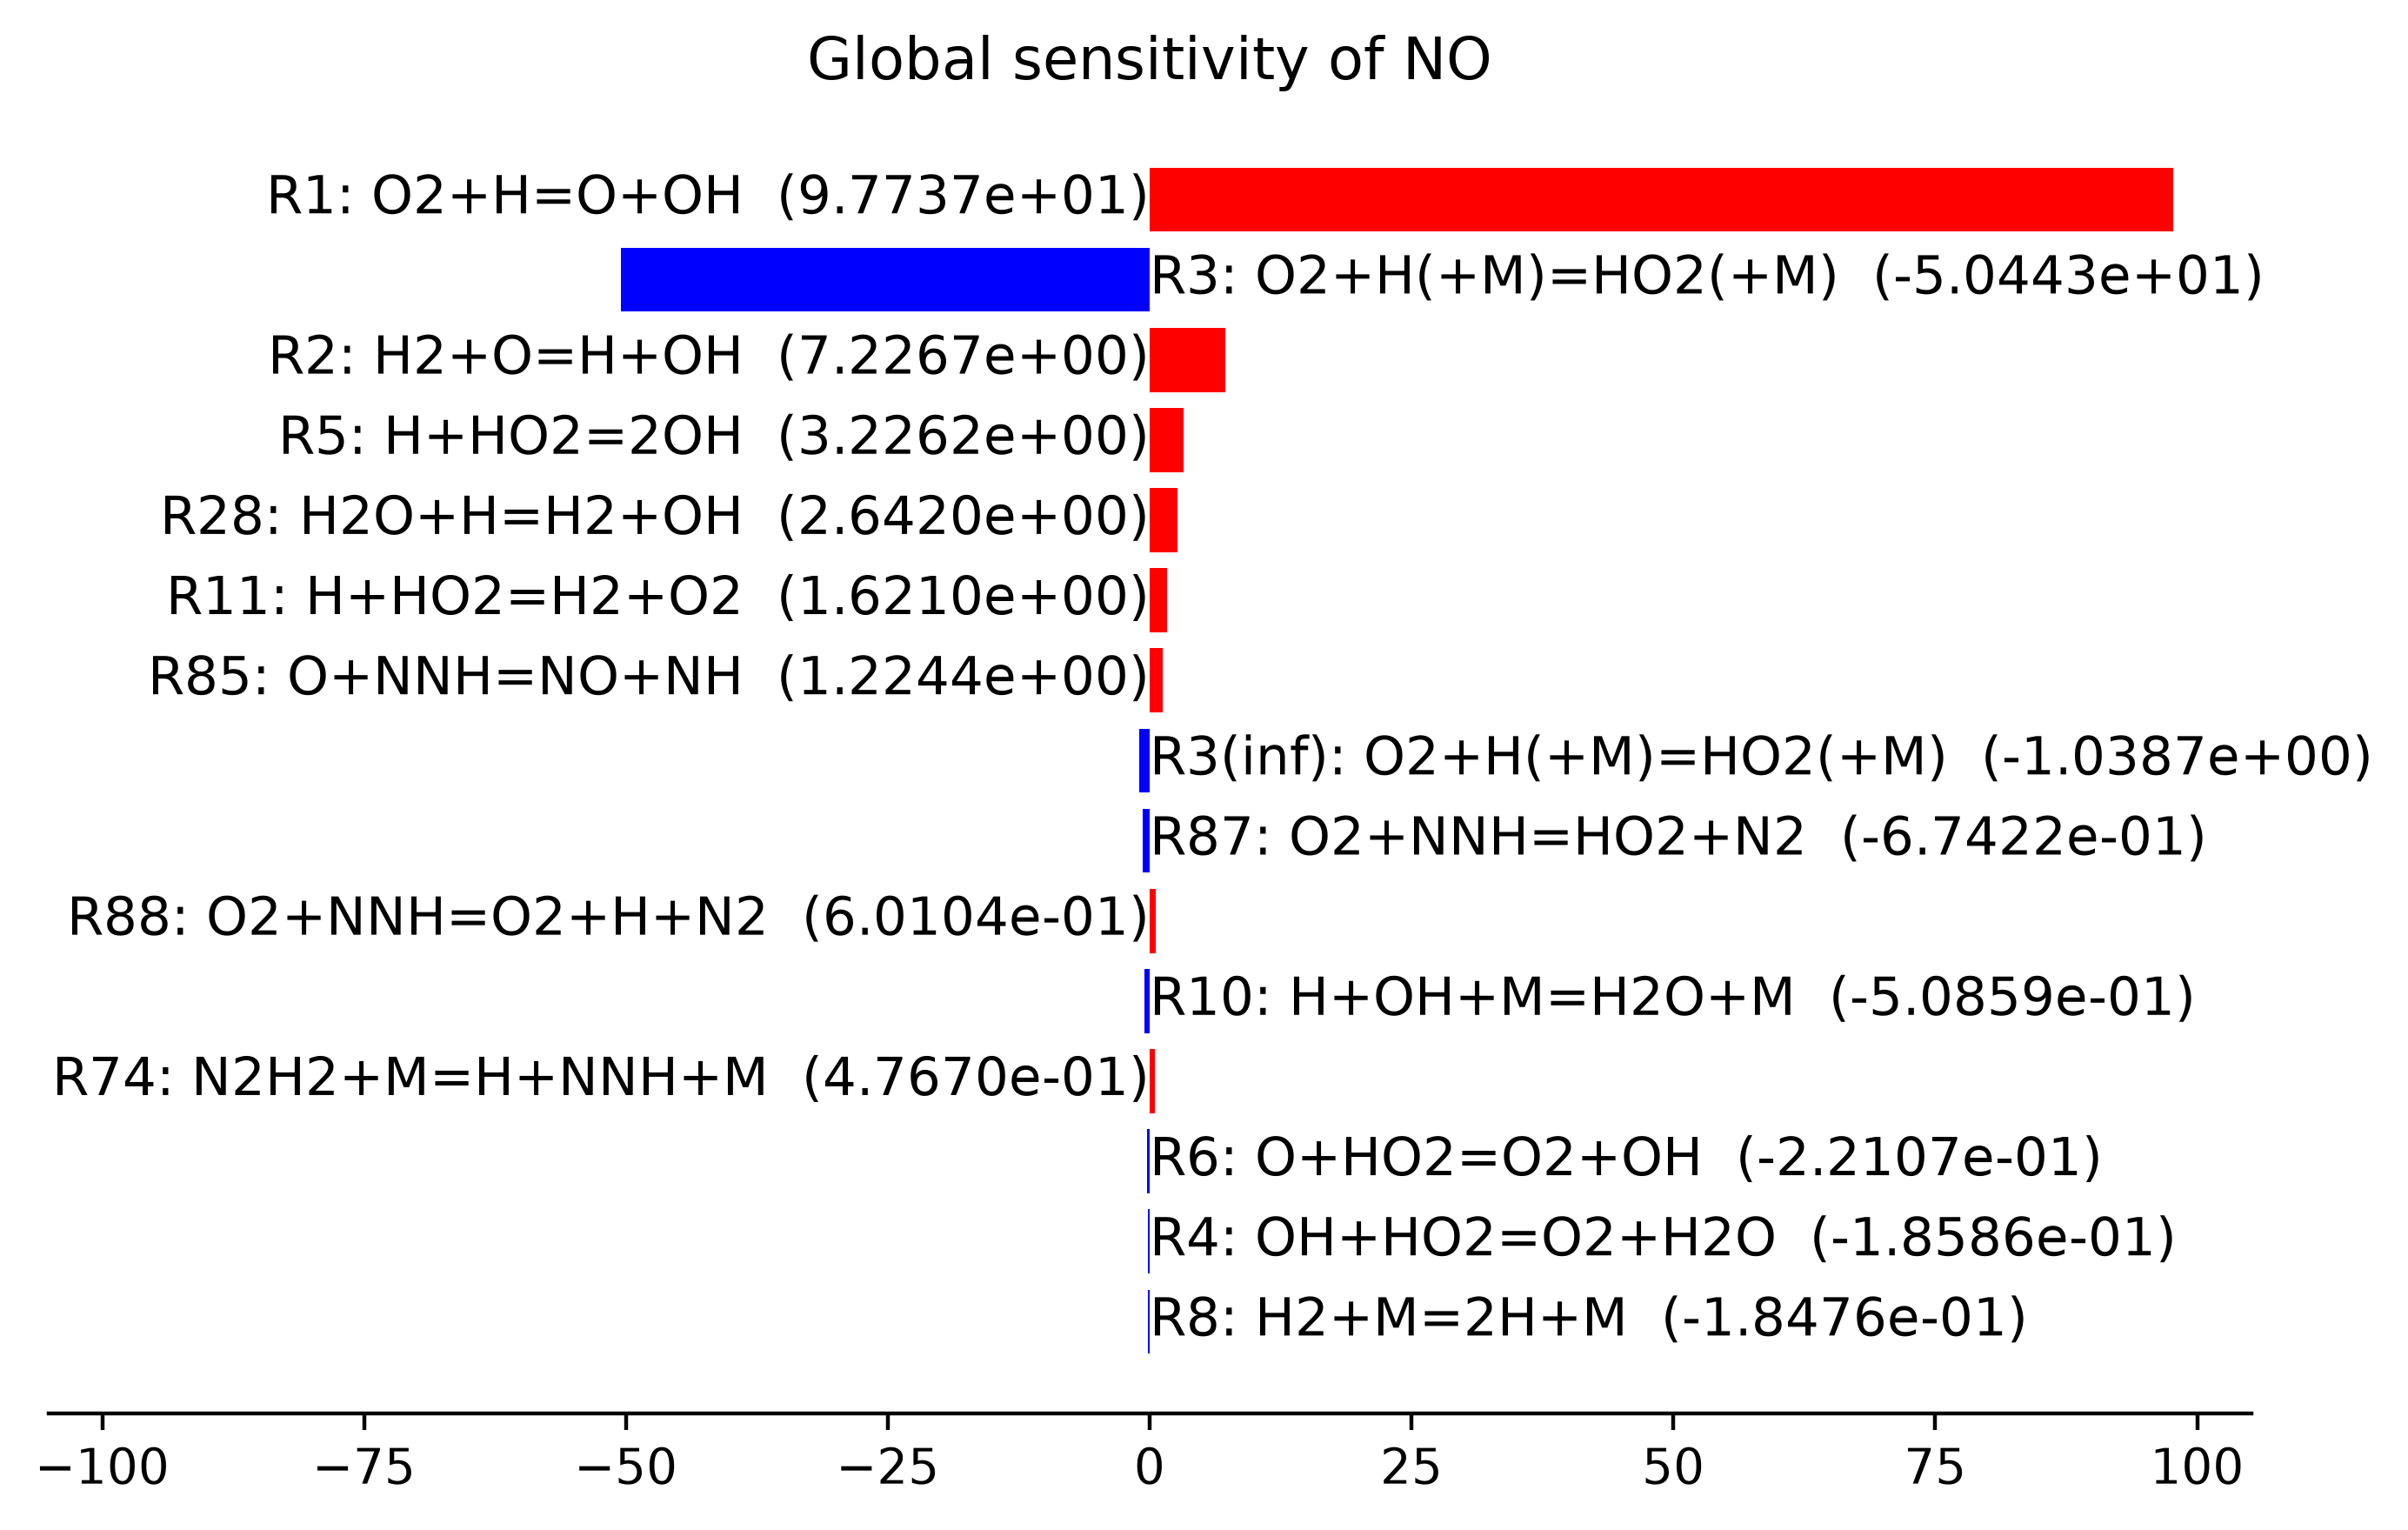
\includegraphics[width=0.75\textwidth]{figures/sensitivity_bars.png}
\caption{Global sensitivity of NO, plotted with \texttt{plot\_bars}.}
\end{figure}

\pymethod{SensitivityAnalysis\_Surface(target, sensitivity\_type="global", \\ ordering\_type="peak-values", normalization\_type="max-value", local\_value=0, \\ lower\_value=0, upper\_value=0, number\_of\_reactions=10, \\ heterogeneous\_sensitivity=False) -> dict}

Same as \pkg{SensitivityAnalysis}, for coupled gas+surface mechanisms.

\begin{params}
\item \pkg{heterogeneous\_sensitivity} (\textit{bool}) --- run the analysis
  on the surface reaction set (\pkg{True}) or the gas set (\pkg{False}).
\item (remaining parameters as in \pkg{SensitivityAnalysis}.)
\end{params}
\returns same \pkg{dict} shape, names resolved against the selected phase.

\pymethod{SensitivityCoefficients(target, normalization\_type, reaction\_name=None, reaction\_index=None) -> list}

\vspace{-1mm}
\textit{Note: kept for backward compatibility; largely superseded by
\pkg{SensitivityAnalysis} and not updated for heterogeneous mechanisms ---
prefer \pkg{SensitivityAnalysis} for new code.}
% LG I am not sure whether this is actually just old code.

\begin{params}
\item \pkg{target} (\textit{str}) --- target species.
\item \pkg{normalization\_type} (\textit{str}).
\item \pkg{reaction\_name} (\textit{str}, optional) --- resolved to
  \pkg{reaction\_index} if given.
\item \pkg{reaction\_index} (\textit{int}, optional).
\end{params}
\returns \textit{list[float]}, sensitivity-coefficient profile for the
selected reaction.

\chapter{Elementary Flux Analysis}

\pymethod{FluxAnalysis(species, element, flux\_analysis\_type, thickness, thickness\_log\_scale, label\_type, depth=2, width=5, threshold=0, local\_value=0.01) -> graphviz.Digraph}

Builds a species-to-species element-flux diagram (a directed graph) rooted
at \pkg{species}, walked breadth-first.

\begin{params}
\item \pkg{species} (\textit{str}) --- seed species.
\item \pkg{element} (\textit{str}) --- element symbol to track (e.g.\
  \pkg{"C"}, \pkg{"H"}).
\item \pkg{flux\_analysis\_type} (\textit{str}) --- \pkg{"production"} (blue
  arrows, edges reversed so the graph reads "where the element comes from")
  or \pkg{"destruction"} (red arrows, "where the element goes").
\item \pkg{thickness} (\textit{str}) --- edge-thickness scaling mode (e.g.\
  \pkg{"relative"}).
\item \pkg{thickness\_log\_scale} (\textit{bool}) --- use a log scale for
  edge thickness.
\item \pkg{label\_type} (\textit{str}) --- edge label content mode (e.g.\
  \pkg{"relative"}).
\item \pkg{depth} (\textit{int}) --- number of graph generations to walk
  from the seed.
\item \pkg{width} (\textit{int}) --- maximum outgoing edges kept per node.
\item \pkg{threshold} (\textit{float}) --- minimum edge weight (as a
  fraction of a node's flux) to keep.
\item \pkg{local\_value} (\textit{float}) --- abscissa at which the flux is
  evaluated.
\end{params}
\returns \pkg{graphviz.Digraph}. Display it directly in a notebook
(\pkg{IPython.display.display(G)}), or render to a file with
\pkg{G.render(filename=..., format="png")}.

\begin{figure}[h]
\centering
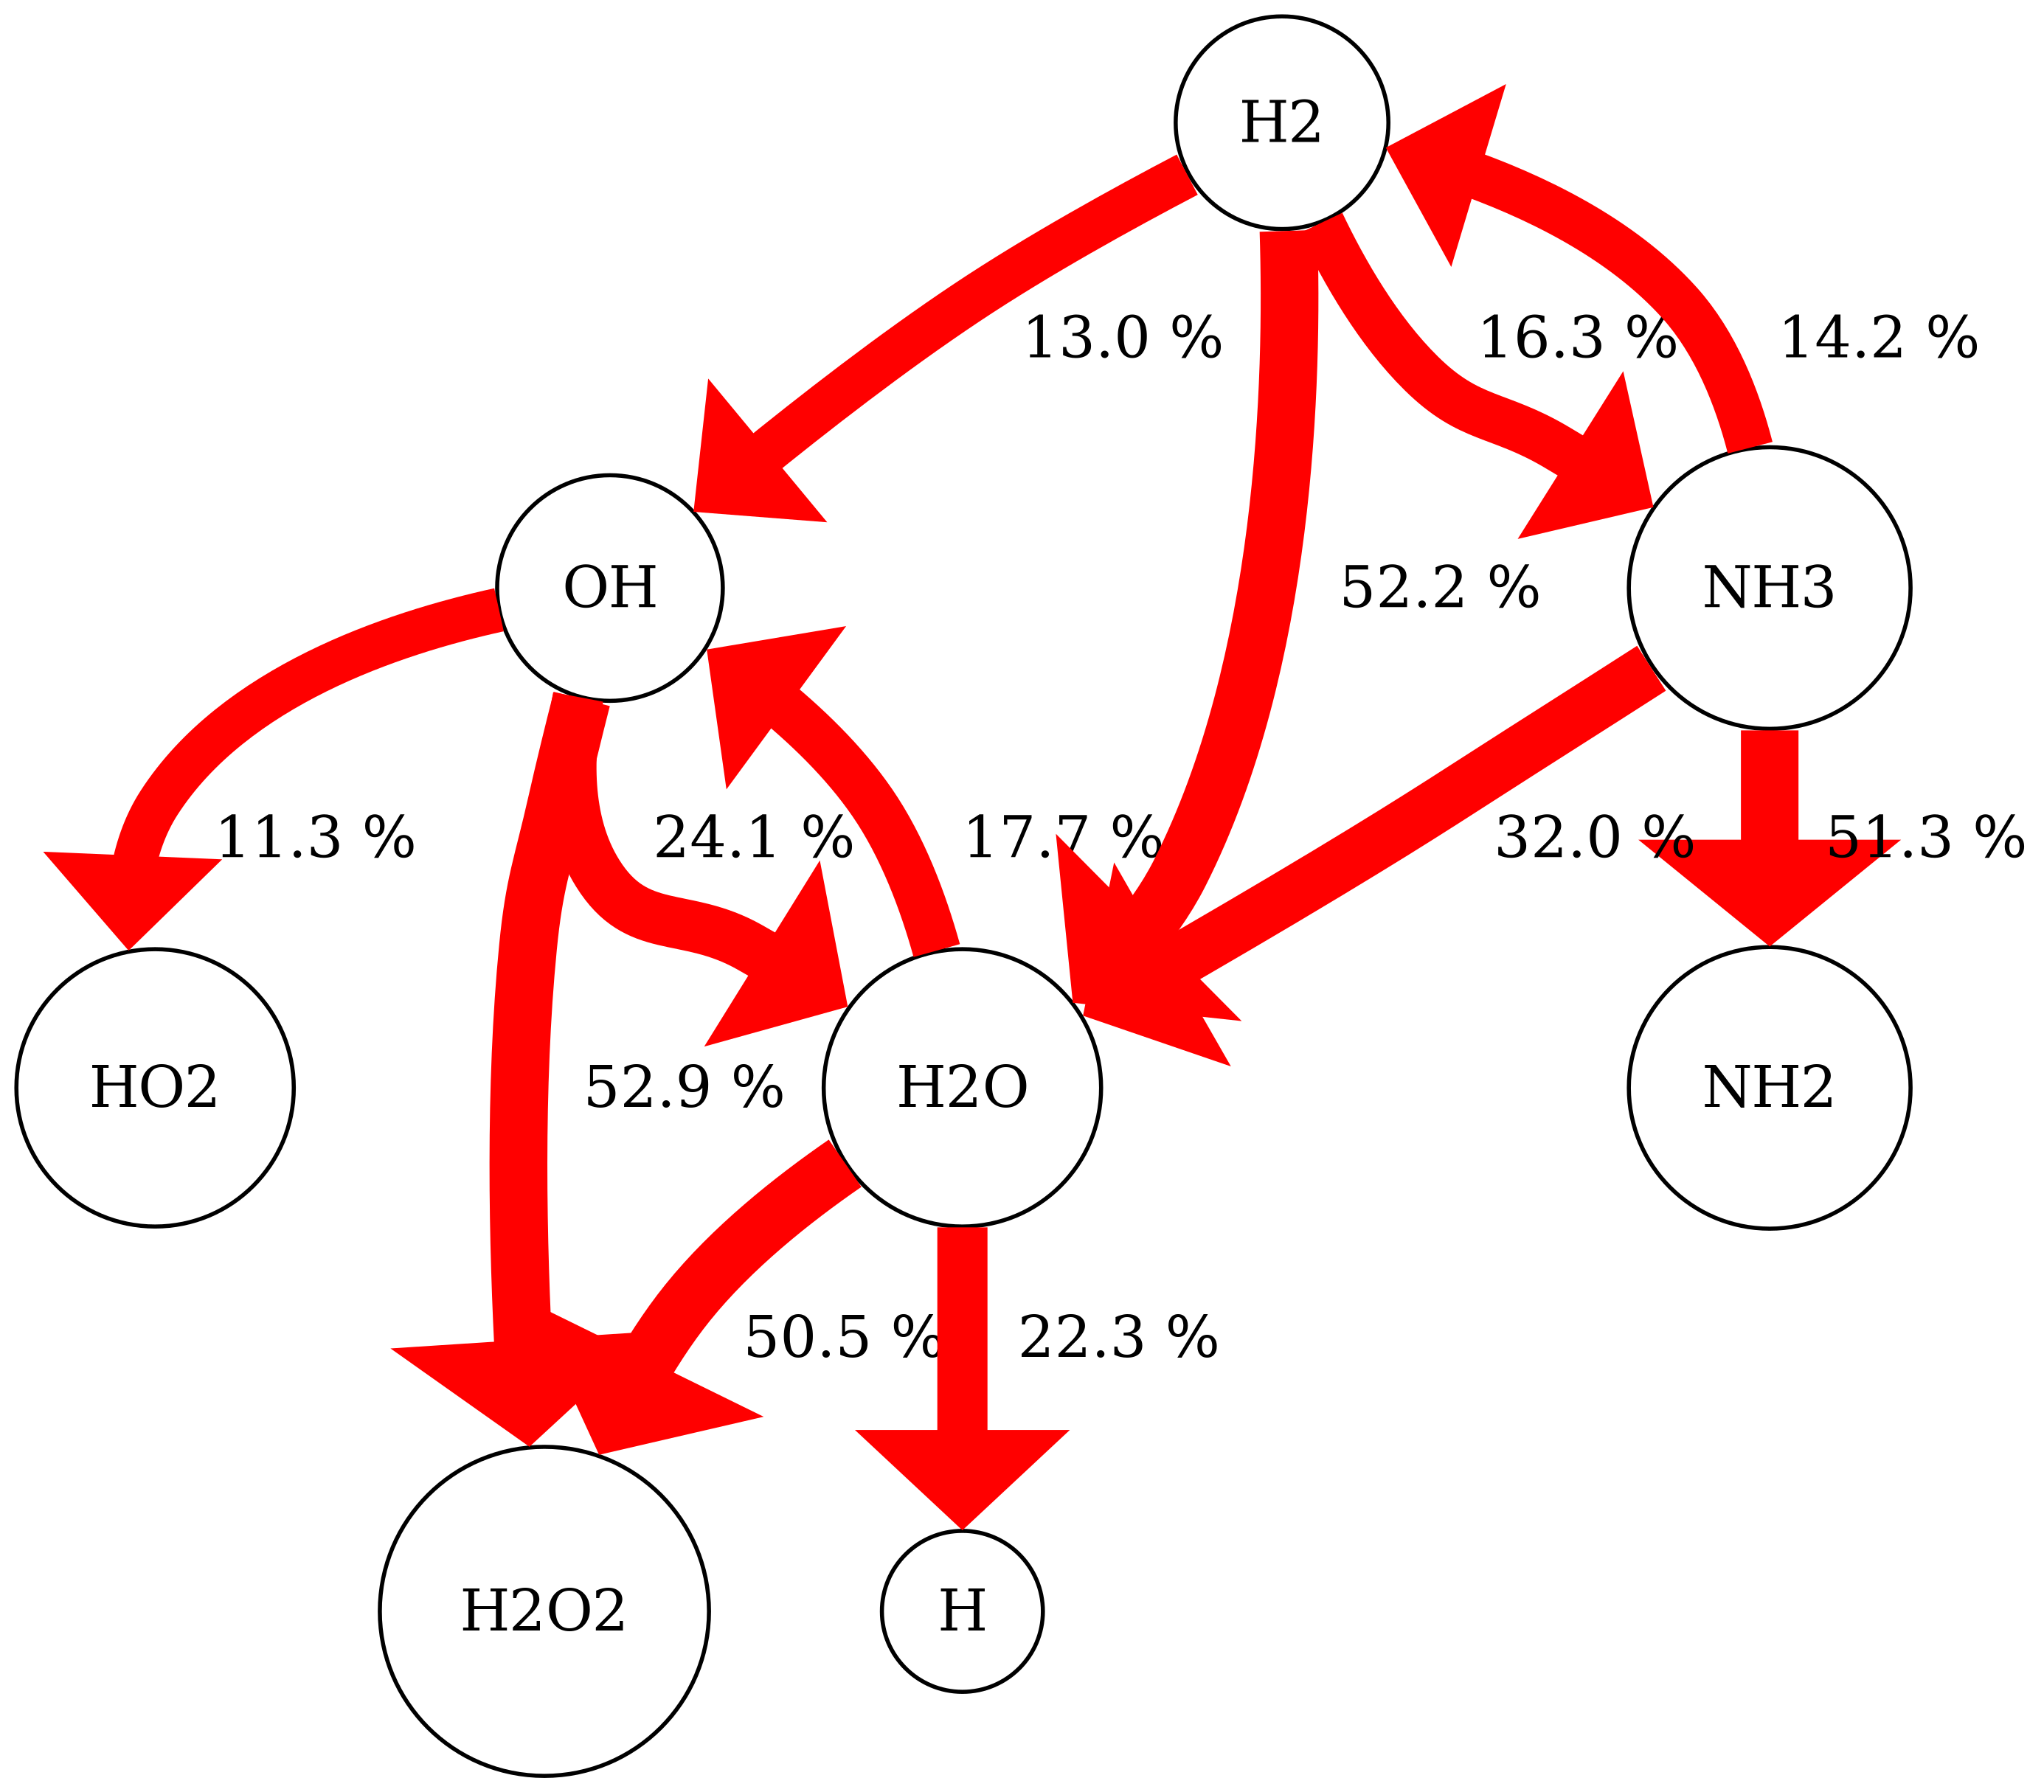
\includegraphics[width=0.5\textwidth]{figures/flux_analysis.png}
\caption{Destruction flux graph of H2 on the element H (depth 1, width 3). Red edges, arrows point toward where the element ends up.}
\end{figure}

Switching only \pkg{flux\_analysis\_type} to \pkg{"production"} keeps every
other parameter identical but answers the complementary question --- "where
does this element in H2 come from" --- and is drawn in blue with edges
reversed so the diagram still reads left-to-right as a flow \emph{into} the
seed species:

\begin{figure}[h]
\centering
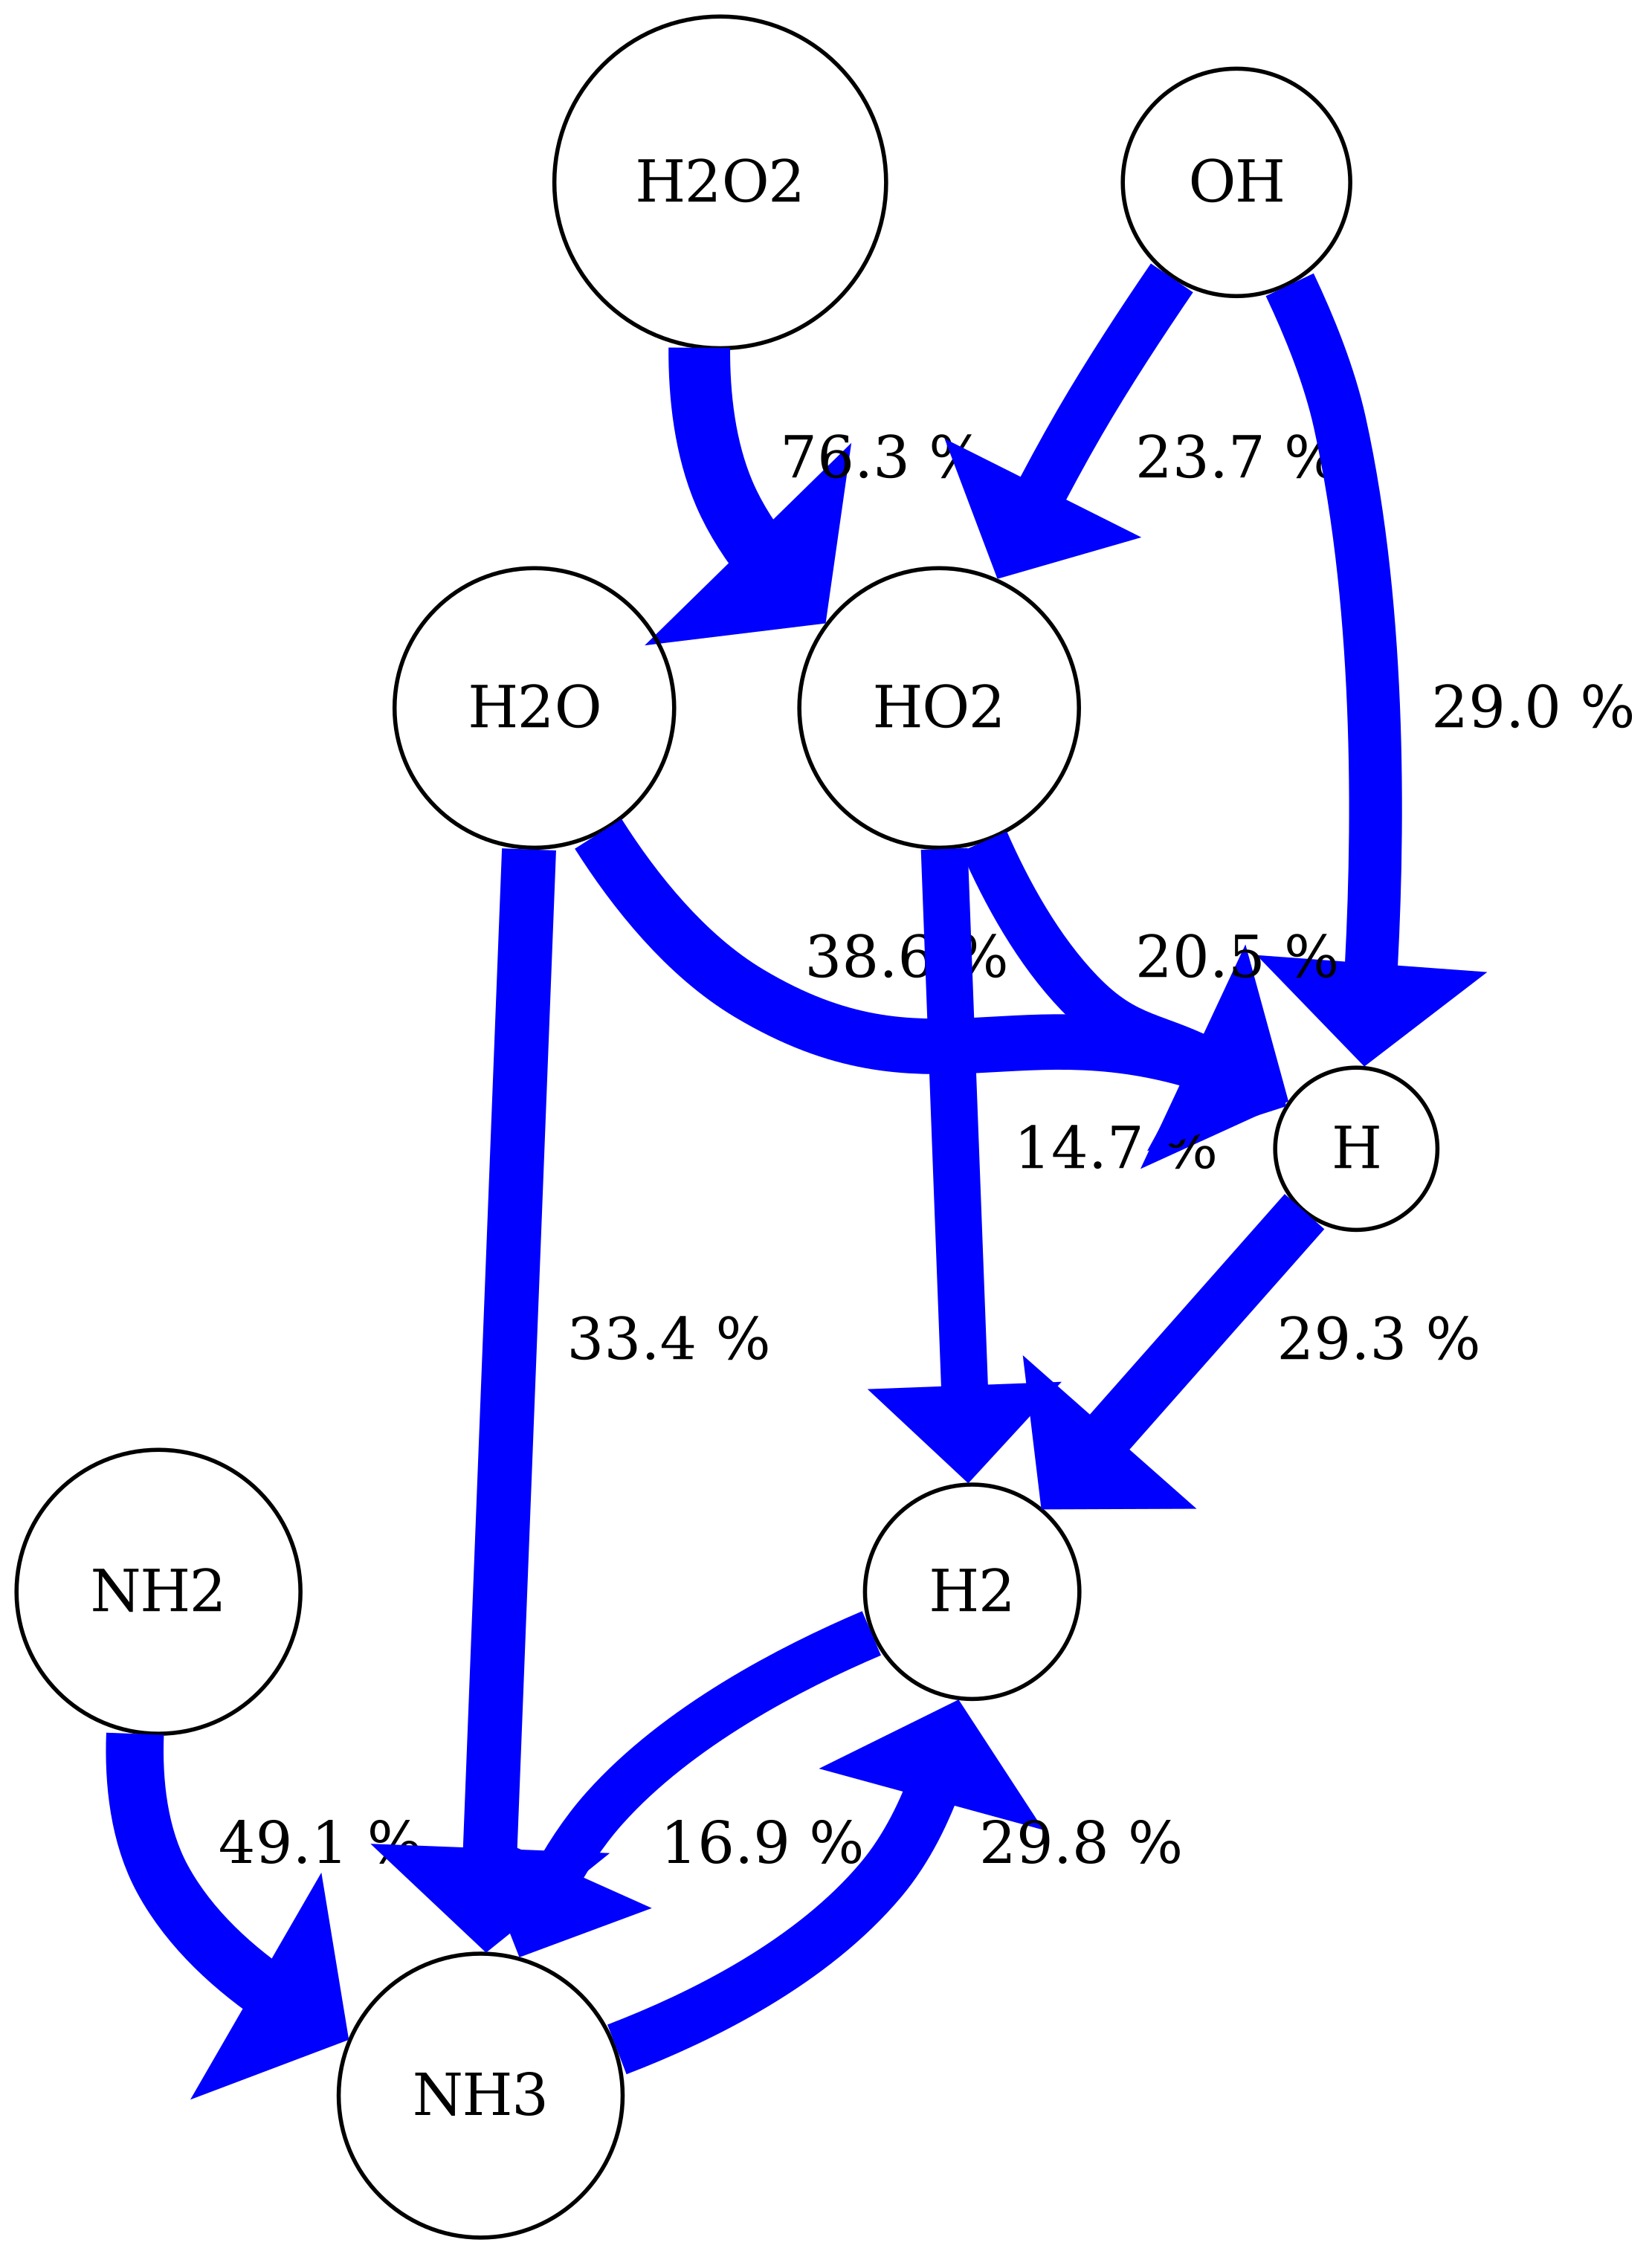
\includegraphics[width=0.55\textwidth]{figures/flux_analysis_production.png}
\caption{Production flux graph of H2 on the element H, same parameters as above except \texttt{flux\_analysis\_type="production"}. Blue edges.}
\end{figure}

\chapter{Species-Class Analysis}

Available when the mechanism's \pkg{kinetics.xml} contains a
\pkg{<SpeciesClasses>} block, partitioning species into named classes (e.g.\
\pkg{C1}, \pkg{AROMATICS}, \pkg{SOOT-*}). All methods below raise a plain
Python exception (not a segfault) if the mechanism has no such block.

\pymethod{ElementalDistributionByClass(element, normalize=True) -> pandas.DataFrame}

Distribution of an atomic element across the species classes, along the
independent variable.

\begin{params}
\item \pkg{element} (\textit{str}) --- element symbol, as written in the
  mechanism (e.g.\ \pkg{"C"}, \pkg{"H"}, \pkg{"O"}).
\item \pkg{normalize} (\textit{bool}) --- if \pkg{True}, every row sums to 1
  (fraction of the element carried by each class at that point); if
  \pkg{False}, values are moles of the element per unit mass of mixture
  (conserved across all phases, not necessarily within a single phase, e.g.\
  under surface deposition).
\end{params}
\returns \pkg{DataFrame} indexed by the independent variable, one column per
class.

\begin{figure}[h]
\centering
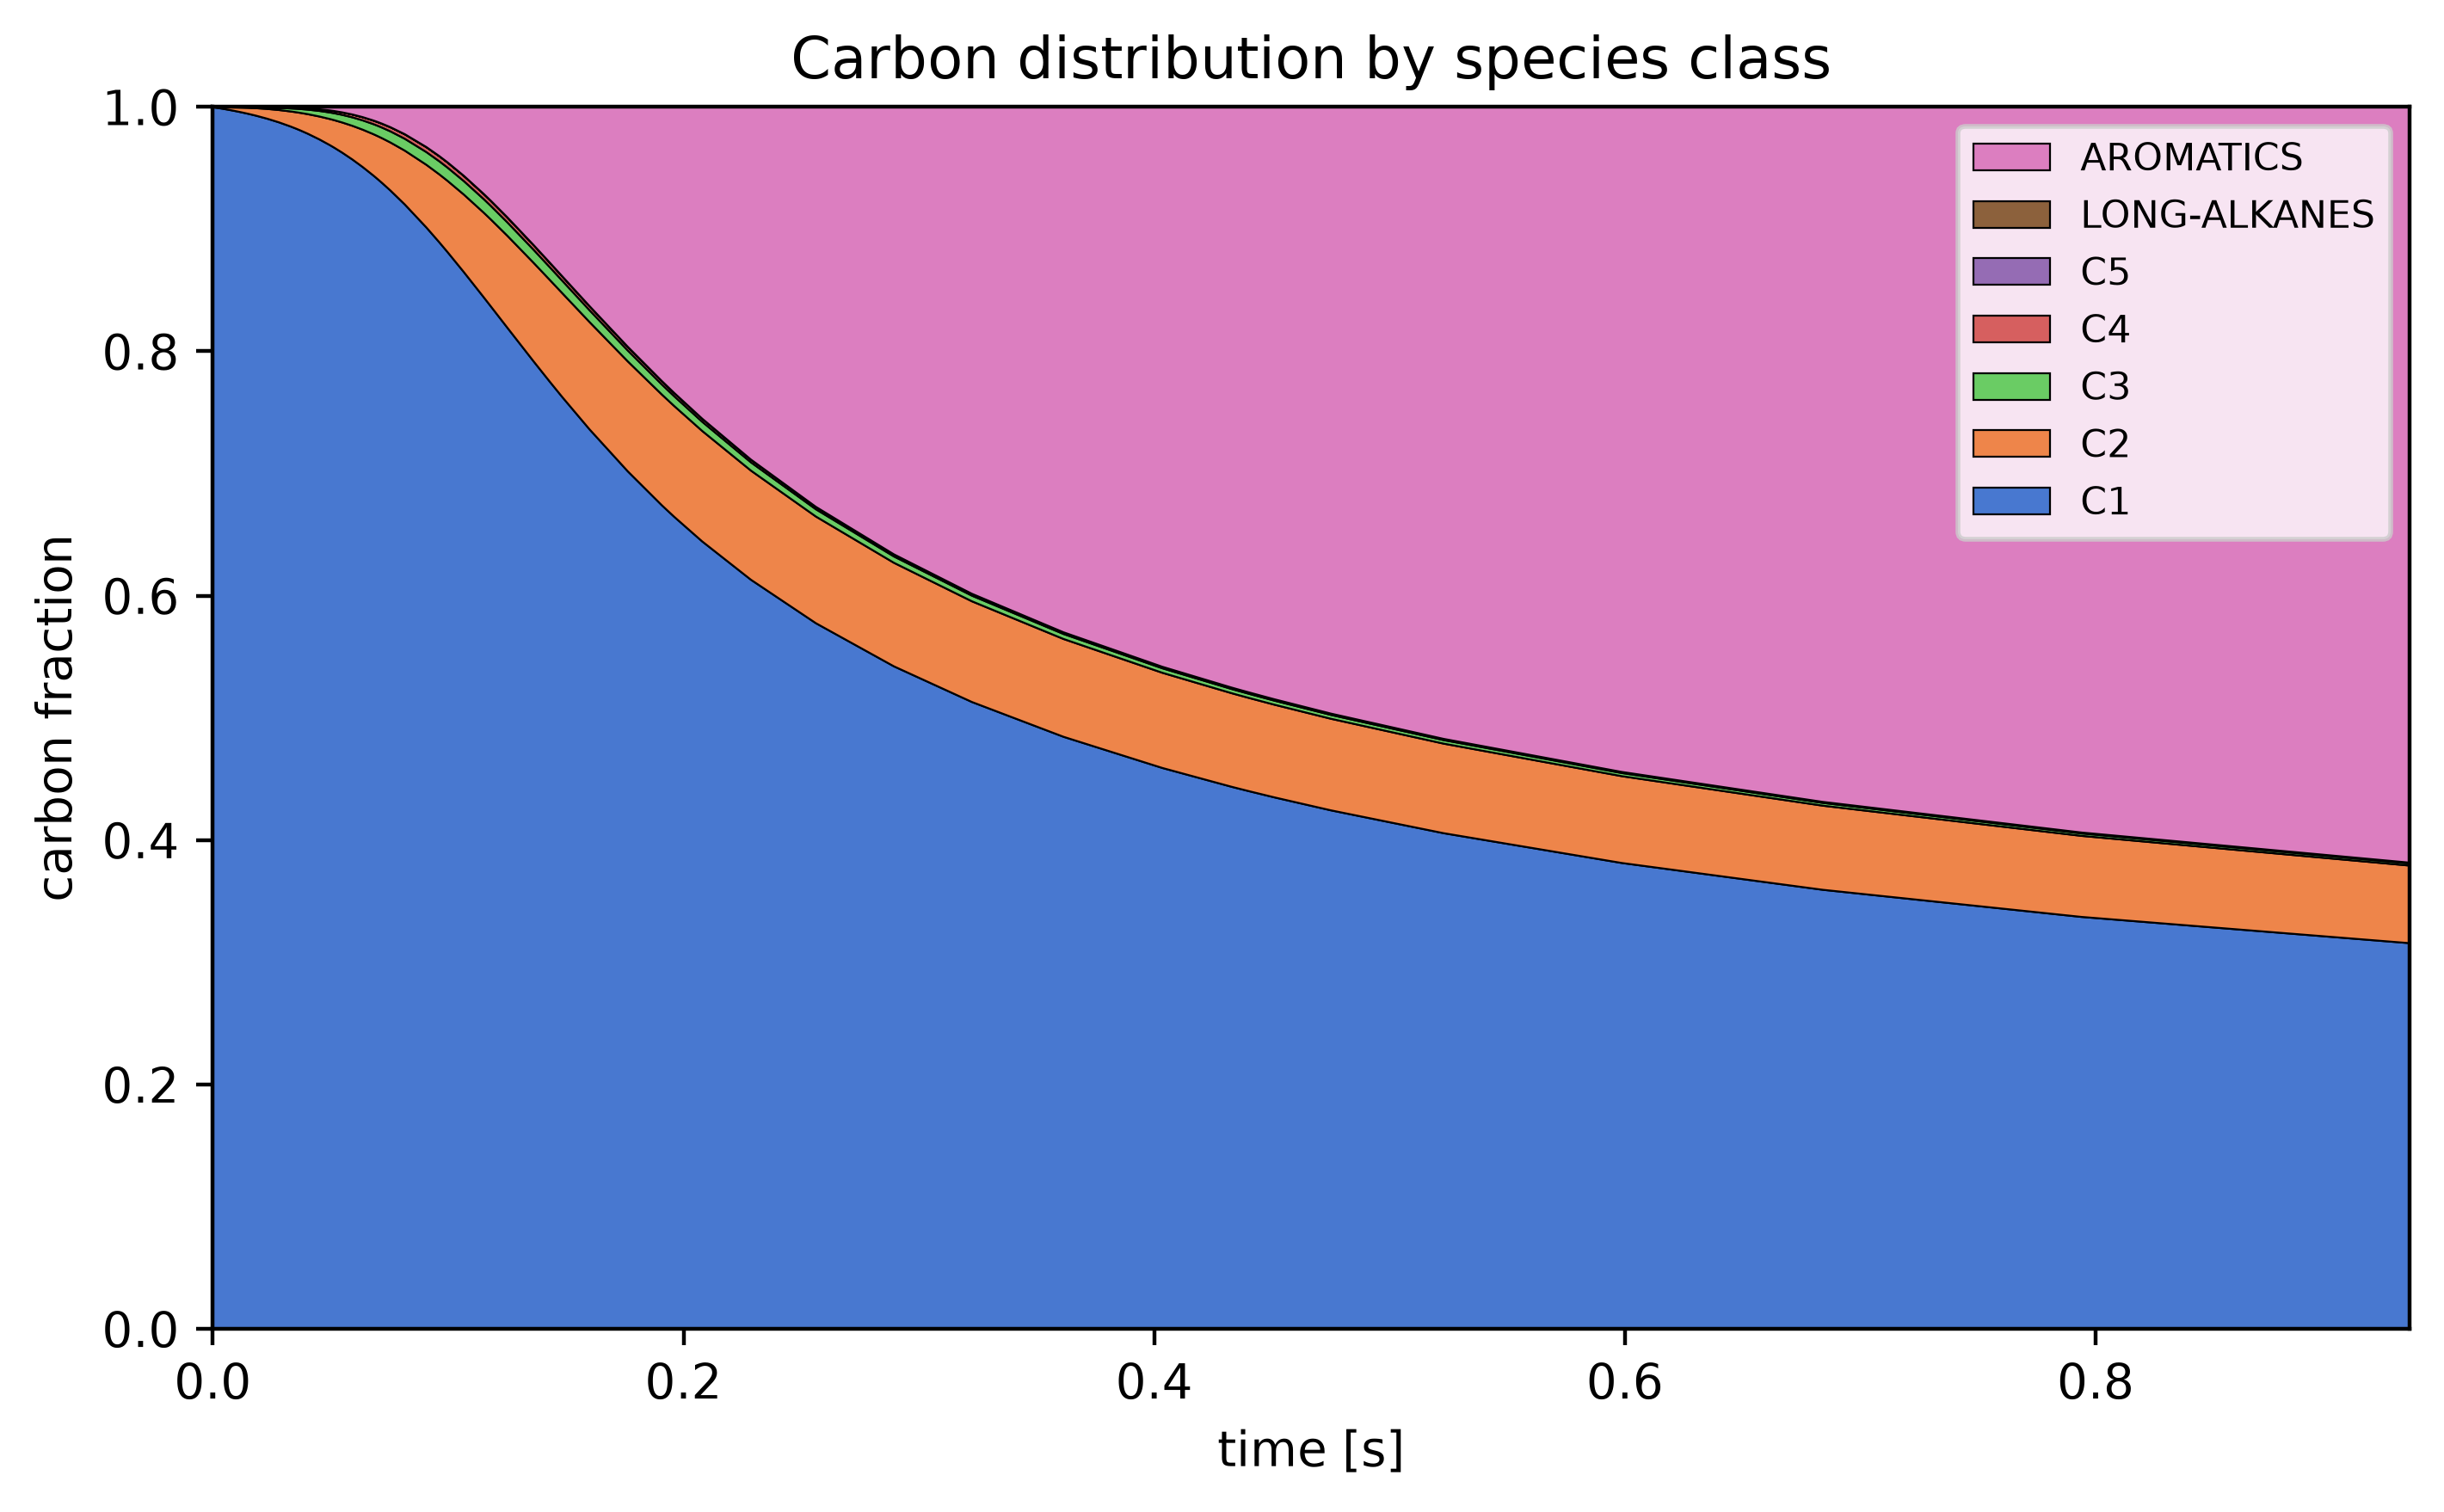
\includegraphics[width=0.75\textwidth]{figures/species_class_distribution.png}
\caption{Carbon distribution across species classes over time, plotted with \texttt{plot\_class\_distribution} for a $CH_4$ pyrolysis case.}
\end{figure}

\pymethod{ElementMolesBySpecies(element) -> pandas.DataFrame}

Per-species (not per-class) view of the same underlying computation ---
every species in the mechanism, classified or not. Does \emph{not} require
a \pkg{<SpeciesClasses>} block.

\begin{params}
\item \pkg{element} (\textit{str}) --- element symbol.
\end{params}
\returns \pkg{DataFrame} indexed by the independent variable, one column per
species: moles of the element per unit mass of mixture.

\pymethod{FluxAnalysisByClass(element, flux\_analysis\_type, class\_name=None, \\ species\_name=None, flux\_per\_class=True, thickness="relative", \\ thickness\_log\_scale=True, label\_type="relative", depth=2, width=3, \\ threshold=0.02, local\_value=0.01, carbon\_weighted=True, auto\_prune\_diagonal=True) -> dict}

Element flux between species \emph{classes} at a point of the independent
variable. The full directed class$\to$class flux matrix is always computed
from every reaction (no species-level pruning); \pkg{depth}/\pkg{width}/
\pkg{threshold} only prune the returned \emph{graph}, walked breadth-first
from a seed class.

\begin{params}
\item \pkg{element}, \pkg{flux\_analysis\_type}, \pkg{thickness},
  \pkg{thickness\_log\_scale}, \pkg{label\_type}, \pkg{depth}, \pkg{width},
  \pkg{threshold}, \pkg{local\_value} --- as in \pkg{FluxAnalysis}.
\item \pkg{class\_name} (\textit{str}) --- seed class name; required (and
  only valid) when \pkg{flux\_per\_class=True}.
\item \pkg{species\_name} (\textit{str}) --- seed species name (the walk
  starts from the class containing it); required (and only valid) when
  \pkg{flux\_per\_class=False}.
\item \pkg{flux\_per\_class} (\textit{bool}) --- selects which of
  \pkg{class\_name}/\pkg{species\_name} is used as the seed (exactly one of
  the two must be given, matching this flag; a \pkg{ValueError} is raised
  otherwise).
\item \pkg{carbon\_weighted} (\textit{bool}) --- \pkg{True} (default): use
  OpenSMOKE's own carbon-atom-throughput weighting (matches the reference
  flux-analysis map; for a mechanism with lumped soot BINs, the soot-to-soot
  term dominates since it scales with the square of BIN carbon count).
  \pkg{False}: split each reaction's own molar rate by carbon share, bounded
  per reaction, keeping lumped BIN classes visually comparable to small gas
  species.
\item \pkg{auto\_prune\_diagonal} (\textit{bool}) --- if \pkg{True}
  (default), zero the diagonal of the returned matrix (intra-class flux is
  typically far larger than any cross-class term and would otherwise
  dominate a heatmap); the graph never draws self-loops either way. Pass
  \pkg{False} to inspect intra-class activity numerically.
\end{params}
\returns \pkg{dict} with keys \pkg{"matrix"} (\pkg{DataFrame}, rows = source
class, columns = target class, full directed flux) and \pkg{"graph"}
(\pkg{graphviz.Digraph}, the pruned walk).

\begin{figure}[h]
\centering
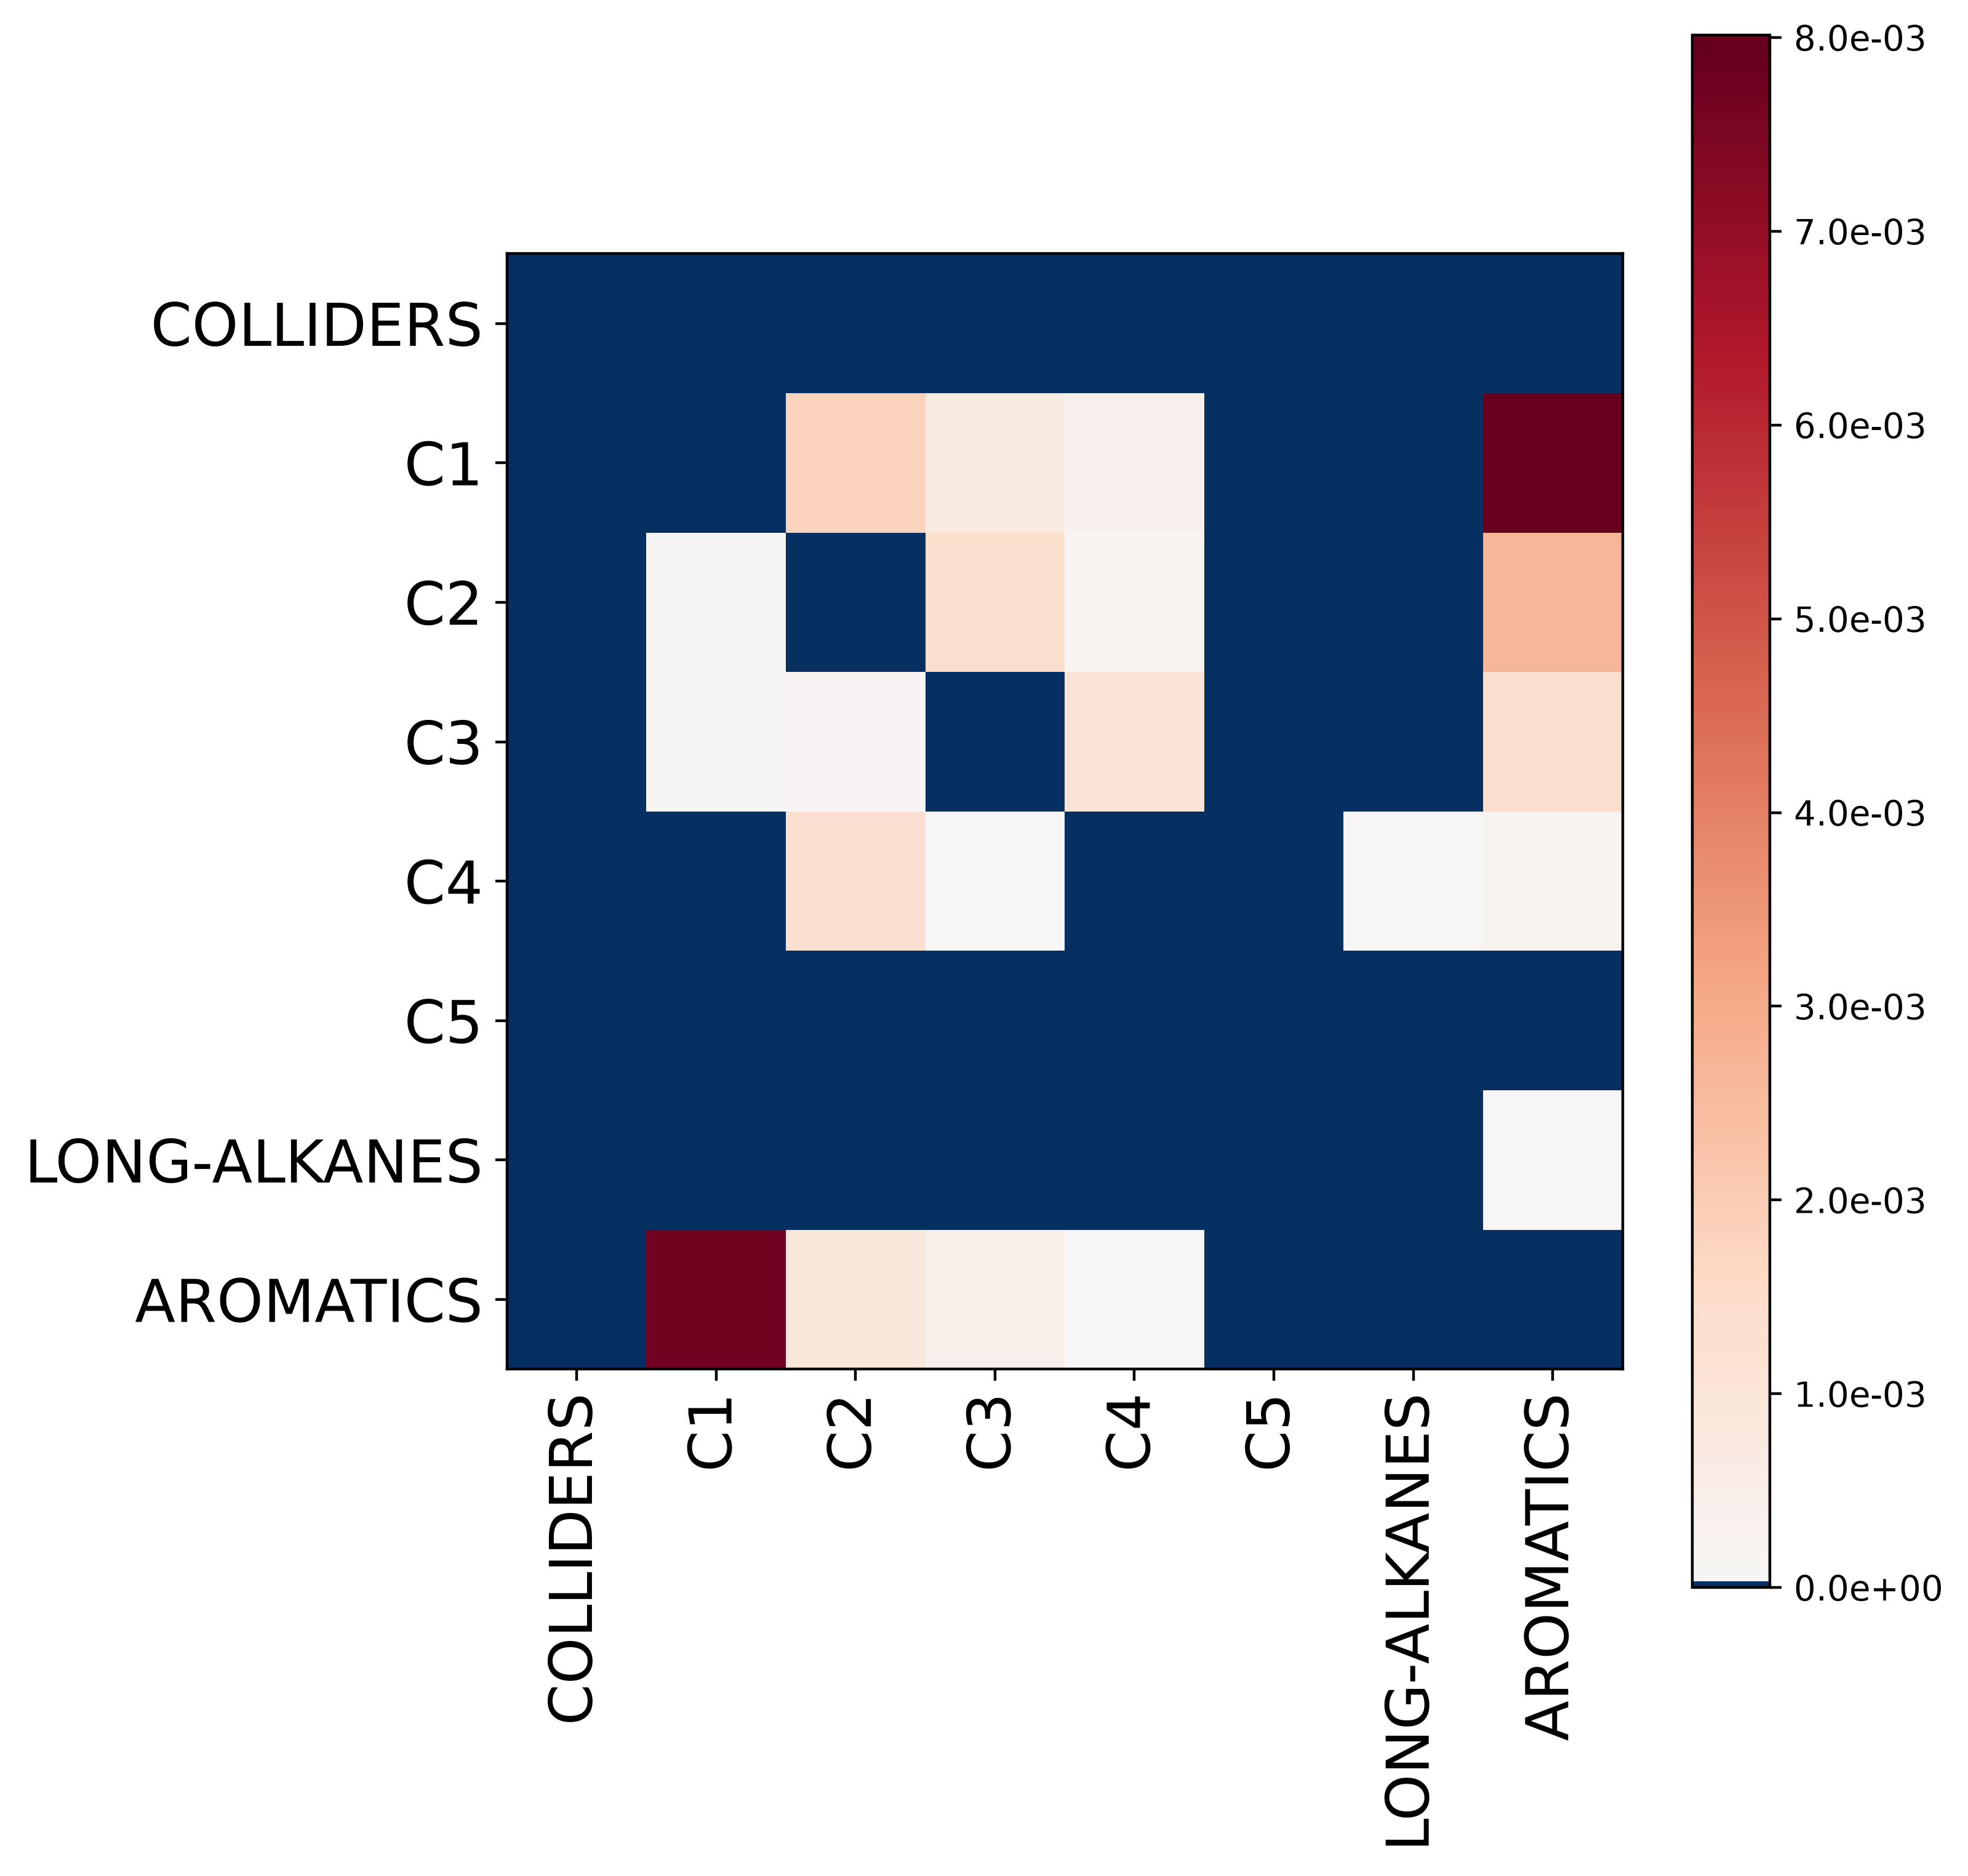
\includegraphics[width=0.85\textwidth]{figures/flux_by_class_heatmap.png}
\caption{Class-to-class carbon flux matrix (destruction, seeded from class C2), plotted with \texttt{plot\_heatmap}.}
\end{figure}

\chapter{Soot Post-Processing}

\pymethod{PostProcessor.dfSootProperties}

Attribute (not a method), set at construction time. A \pkg{pandas.DataFrame}
with one row per BIN, columns matching OpenSMOKE's \pkg{BinProperties.txt}
(\pkg{Bin\_index}, \pkg{Bin\_name}, \pkg{nC[-]}, \pkg{nH[-]}, \pkg{nO[-]},
\pkg{H/C[-]}, \pkg{MW[kg/kmol]}, \pkg{density[kg/m3]}, \pkg{mass[kg]},
\pkg{volume[m3]}, \pkg{Dsph[m]}, \pkg{Dcol[m]}, \pkg{Dpp[m]}, \pkg{Df[-]},
\pkg{numPP[\#]}, \pkg{Bin\_section}). \pkg{None} if the mechanism has no
\pkg{<SootProperties>} block.

\pymethod{SootPSD(local\_value=0.0, particle\_type="all", diameter\_type="dmob", \\ min\_section=5, mobility\_exponent=0.45, merge\_tol=0.20) -> pandas.DataFrame}

Soot particle size distribution at a chosen point of the independent
variable.

\begin{params}
\item \pkg{local\_value} (\textit{float}) --- picks the profile point (first
  point whose abscissa $\geq$ \pkg{local\_value}); abscissa is time for a
  reactor, a spatial coordinate for a flame.
\item \pkg{particle\_type} (\textit{str}) --- \pkg{"all"}: every BIN with
  \pkg{Bin\_section} $\geq$ \pkg{min\_section} (nascent BINs with
  \pkg{numPP} $\leq$ 0 counted as one spherule); \pkg{"primary"}: only free
  primary particles (\pkg{numPP == 1}, the classic PPSD), ignoring
  \pkg{min\_section}.
\item \pkg{diameter\_type} (\textit{str}) --- \pkg{"dmob"}: mobility
  diameter $d_m = D_{pp}\cdot numPP^{\text{mobility\_exponent}}$;
  \pkg{"dpp"}: primary-particle diameter; \pkg{"dcol"}: collision diameter;
  \pkg{"dva"}: volume-equivalent sphere diameter (straight from the
  mechanism's \pkg{Bin\_dsph} BIN property, like \pkg{"dpp"}/\pkg{"dcol"}
  --- no transform applied).
\item \pkg{min\_section} (\textit{int}) --- minimum BIN section kept for
  \pkg{particle\_type="all"}.
\item \pkg{mobility\_exponent} (\textit{float}) --- exponent used by the
  mobility-diameter transform.
\item \pkg{merge\_tol} (\textit{float}) --- relative tolerance for merging
  adjacent size bins.
\end{params}
\returns \pkg{DataFrame} with a size column (\pkg{dm[nm]}/\pkg{dpp[nm]}/
\pkg{dcol[nm]}/\pkg{dva[nm]} depending on \pkg{diameter\_type}), \pkg{N[\#/m3]},
\pkg{dN/dlog10(<d>[nm])[\#/m3]} and related columns; the gas state actually
used (T, P, $\rho$, MW, abscissa) is stored in \pkg{df.attrs} --- $\rho$ and
MW are both read directly from the simulation's own \pkg{<additional>}
columns (not re-derived from the ideal-gas law). Raises \pkg{ValueError} if
the mechanism has no \pkg{<SootProperties>} block.

\begin{figure}[h]
\centering
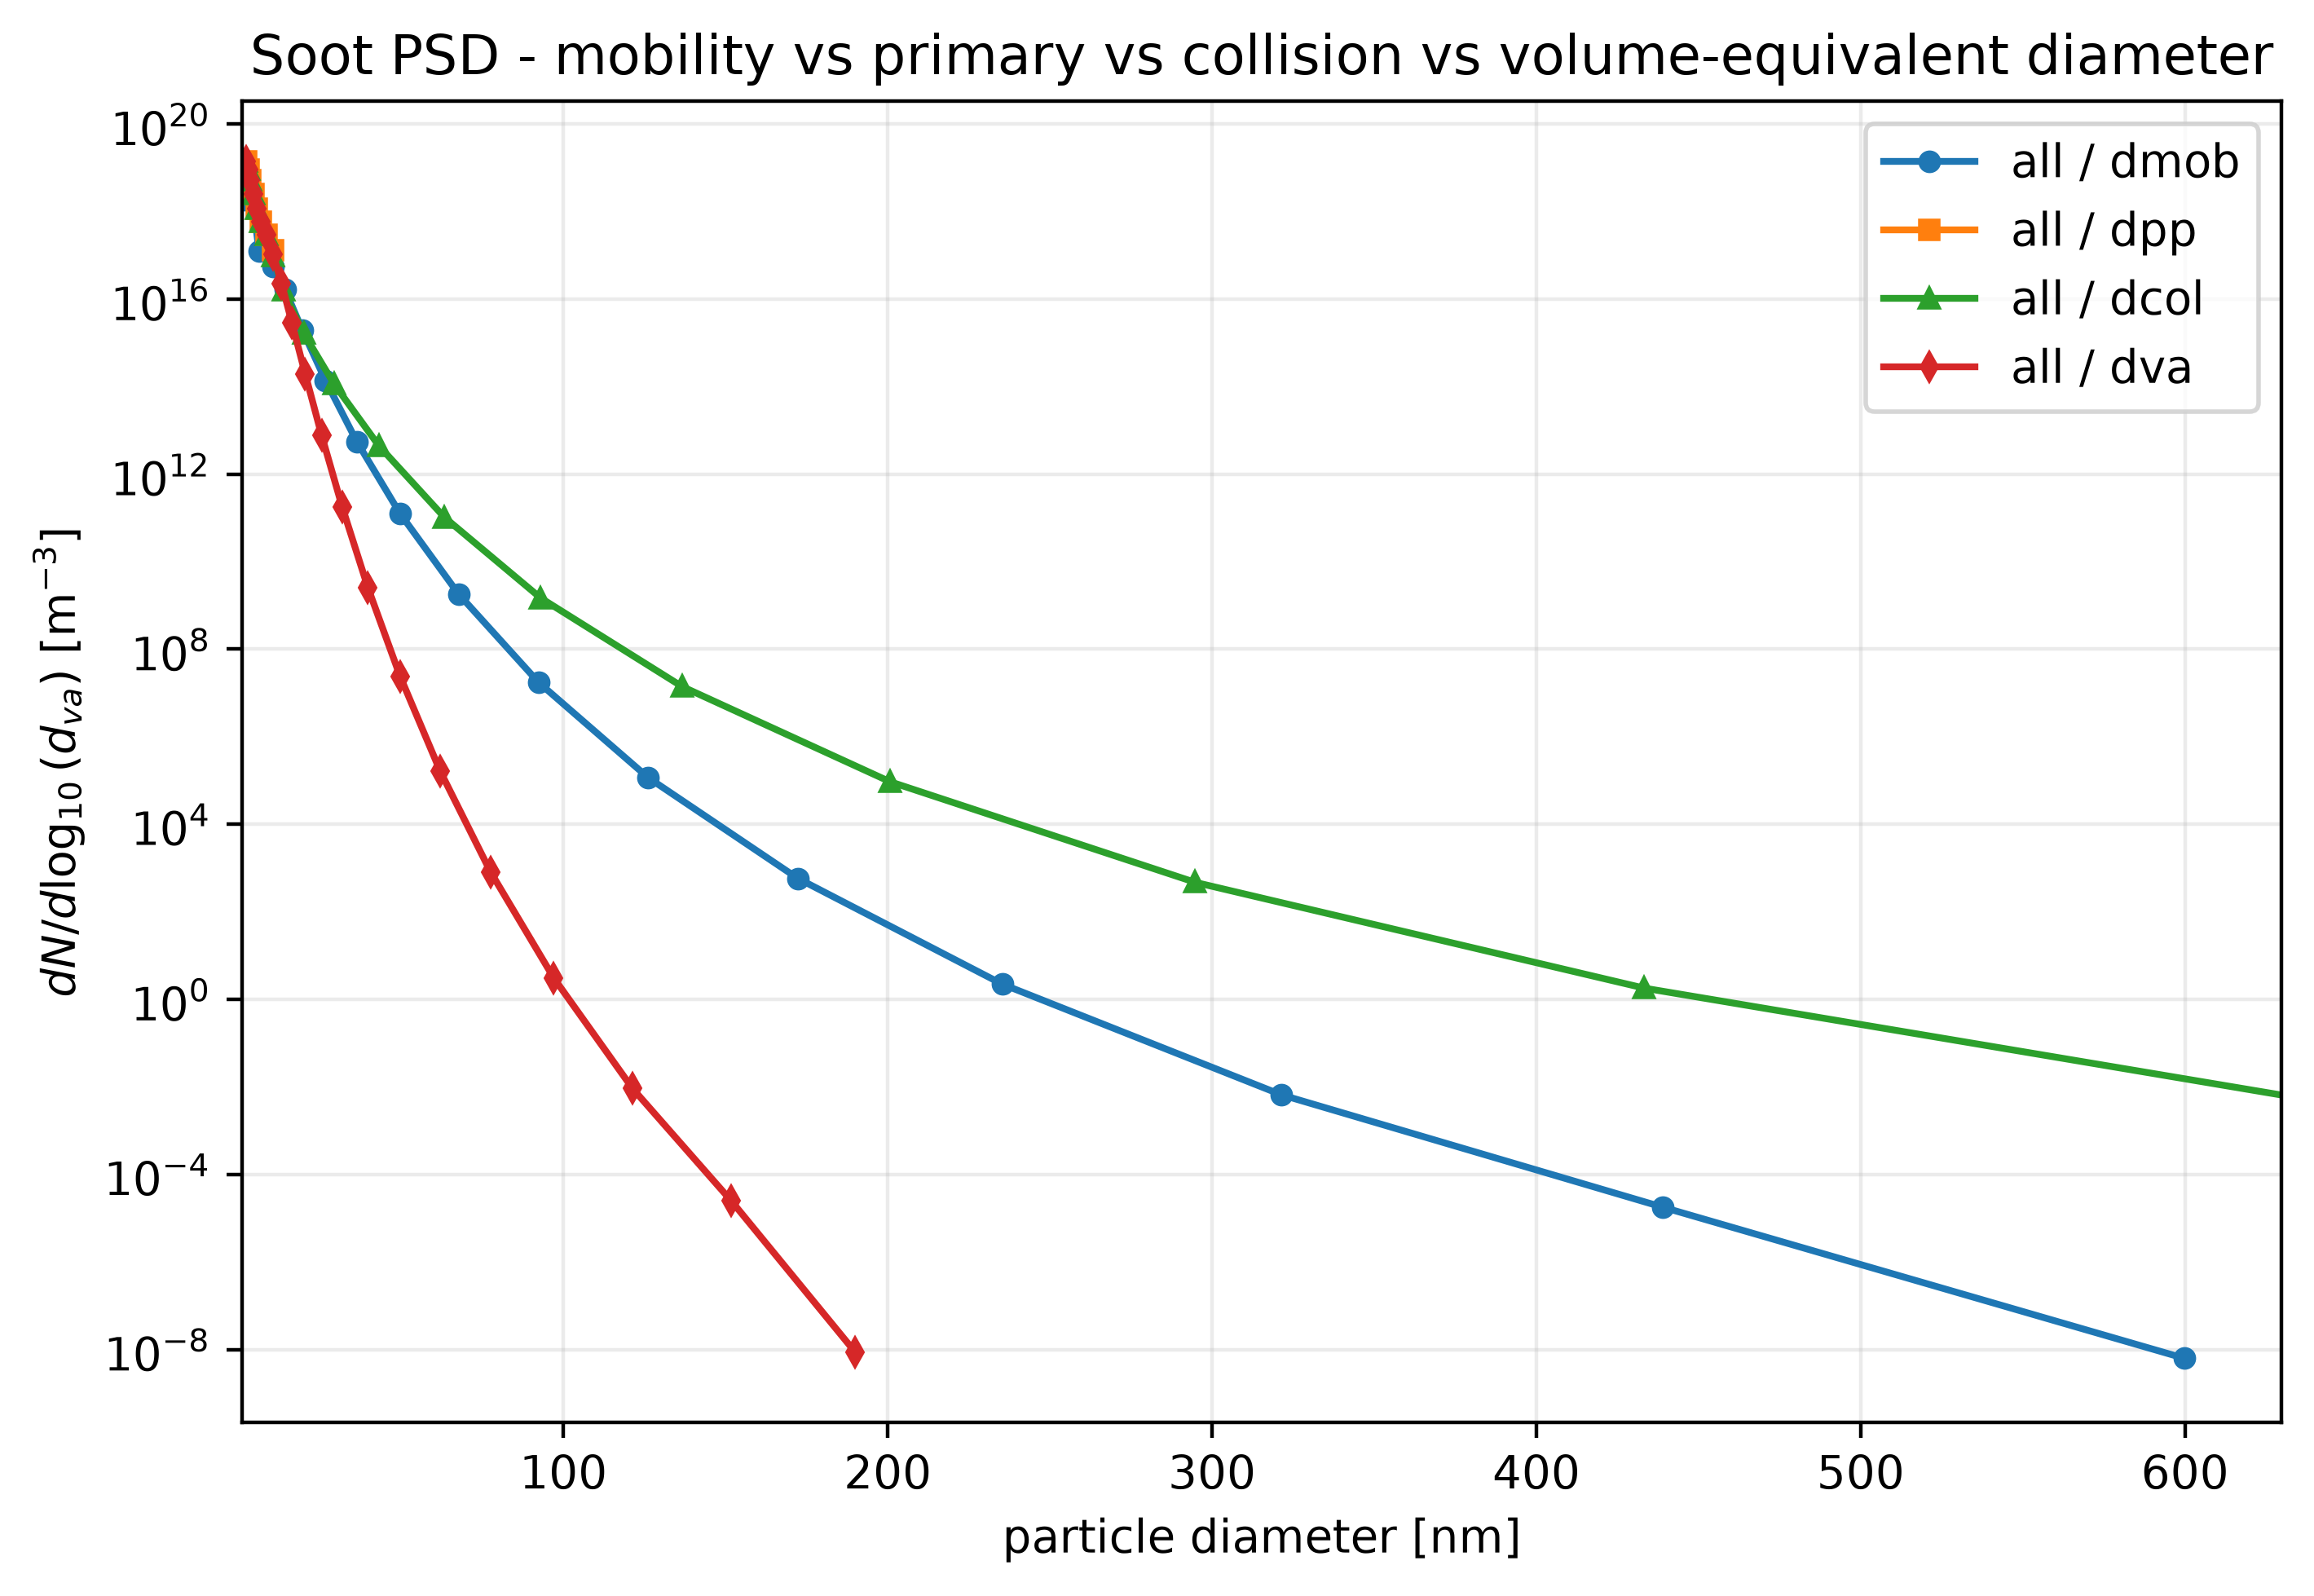
\includegraphics[width=0.75\textwidth]{figures/soot_psd.png}
\caption{Soot PSD at a fixed abscissa, four diameter definitions overlaid with \texttt{plot\_distribution}.}
\end{figure}

\pymethod{getFvSootProfile(as\_dataframe=False, min\_section=5) -> (numpy.ndarray, numpy.ndarray)}

Soot volume fraction $f_v$ [-] along the independent variable: at every point, $\sum_{\text{BIN}} (1/\rho_{\text{BIN}}) \cdot mass_{\text{BIN}}$ over the BINs with \pkg{Bin\_section} $\geq$ \pkg{min\_section} --- the same
definition OpenSMOKE itself uses ($V_{\text{soot}}/V_{\text{tot}}$).

\begin{params}
\item \pkg{as\_dataframe} (\textit{bool}) --- return a \pkg{DataFrame} with
  an \pkg{"fv[-]"} column (plus \pkg{"soot\_mass[kg/m3]"}) instead of the
  \pkg{(x, y)} tuple.
\item \pkg{min\_section} (\textit{int}) --- minimum BIN section included,
  same meaning as in \pkg{SootPSD}.
\end{params}
\returns \pkg{(x, fv)} as \pkg{numpy.ndarray} pairs, or a \pkg{DataFrame}.
\pkg{fv} is \pkg{0} (not \pkg{NaN}) at points with no soot mass. Raises
\pkg{ValueError} if the mechanism has no \pkg{<SootProperties>} block.

\pymethod{getSSASootProfile(as\_dataframe=False, min\_section=5) -> (numpy.ndarray, numpy.ndarray)}

Mean soot specific surface area [m$^2$/kg] along the independent variable:
mass-weighted over the BINs with \pkg{Bin\_section} $\geq$
\pkg{min\_section} (total soot surface / total soot mass), each BIN's own
SSA being $\pi D_{pp}^2 \cdot numPP / mass_{\text{BIN}}$ (\pkg{numPP}
$\leq 0$ counted as 1).

\begin{params}
\item \pkg{as\_dataframe} (\textit{bool}) --- adds a
  \pkg{"soot\_mass[kg/m3]"} column when \pkg{True}.
\item \pkg{min\_section} (\textit{int}).
\end{params}
\returns \pkg{(x, ssa)} pair, or a \pkg{DataFrame}. \pkg{NaN} where there is
no soot.

\pymethod{getHtoCSootProfile(as\_dataframe=False, min\_section=5, weighting="mass") -> (numpy.ndarray, numpy.ndarray)}

Mean soot H/C [-] along the independent variable, over the BINs with
\pkg{Bin\_section} $\geq$ \pkg{min\_section}.

\begin{params}
\item \pkg{as\_dataframe} (\textit{bool}).
\item \pkg{min\_section} (\textit{int}).
\item \pkg{weighting} (\textit{str}) --- \pkg{"mass"}: mass-weighted mean
  of each BIN's own H/C; \pkg{"carbon"}: total H atoms / total C atoms
  across the BINs (the two differ whenever H/C varies across BIN sizes).
\end{params}
\returns \pkg{(x, htoc)} pair, or a \pkg{DataFrame}. \pkg{NaN} where there is
no soot.

\begin{figure}[h]
\centering
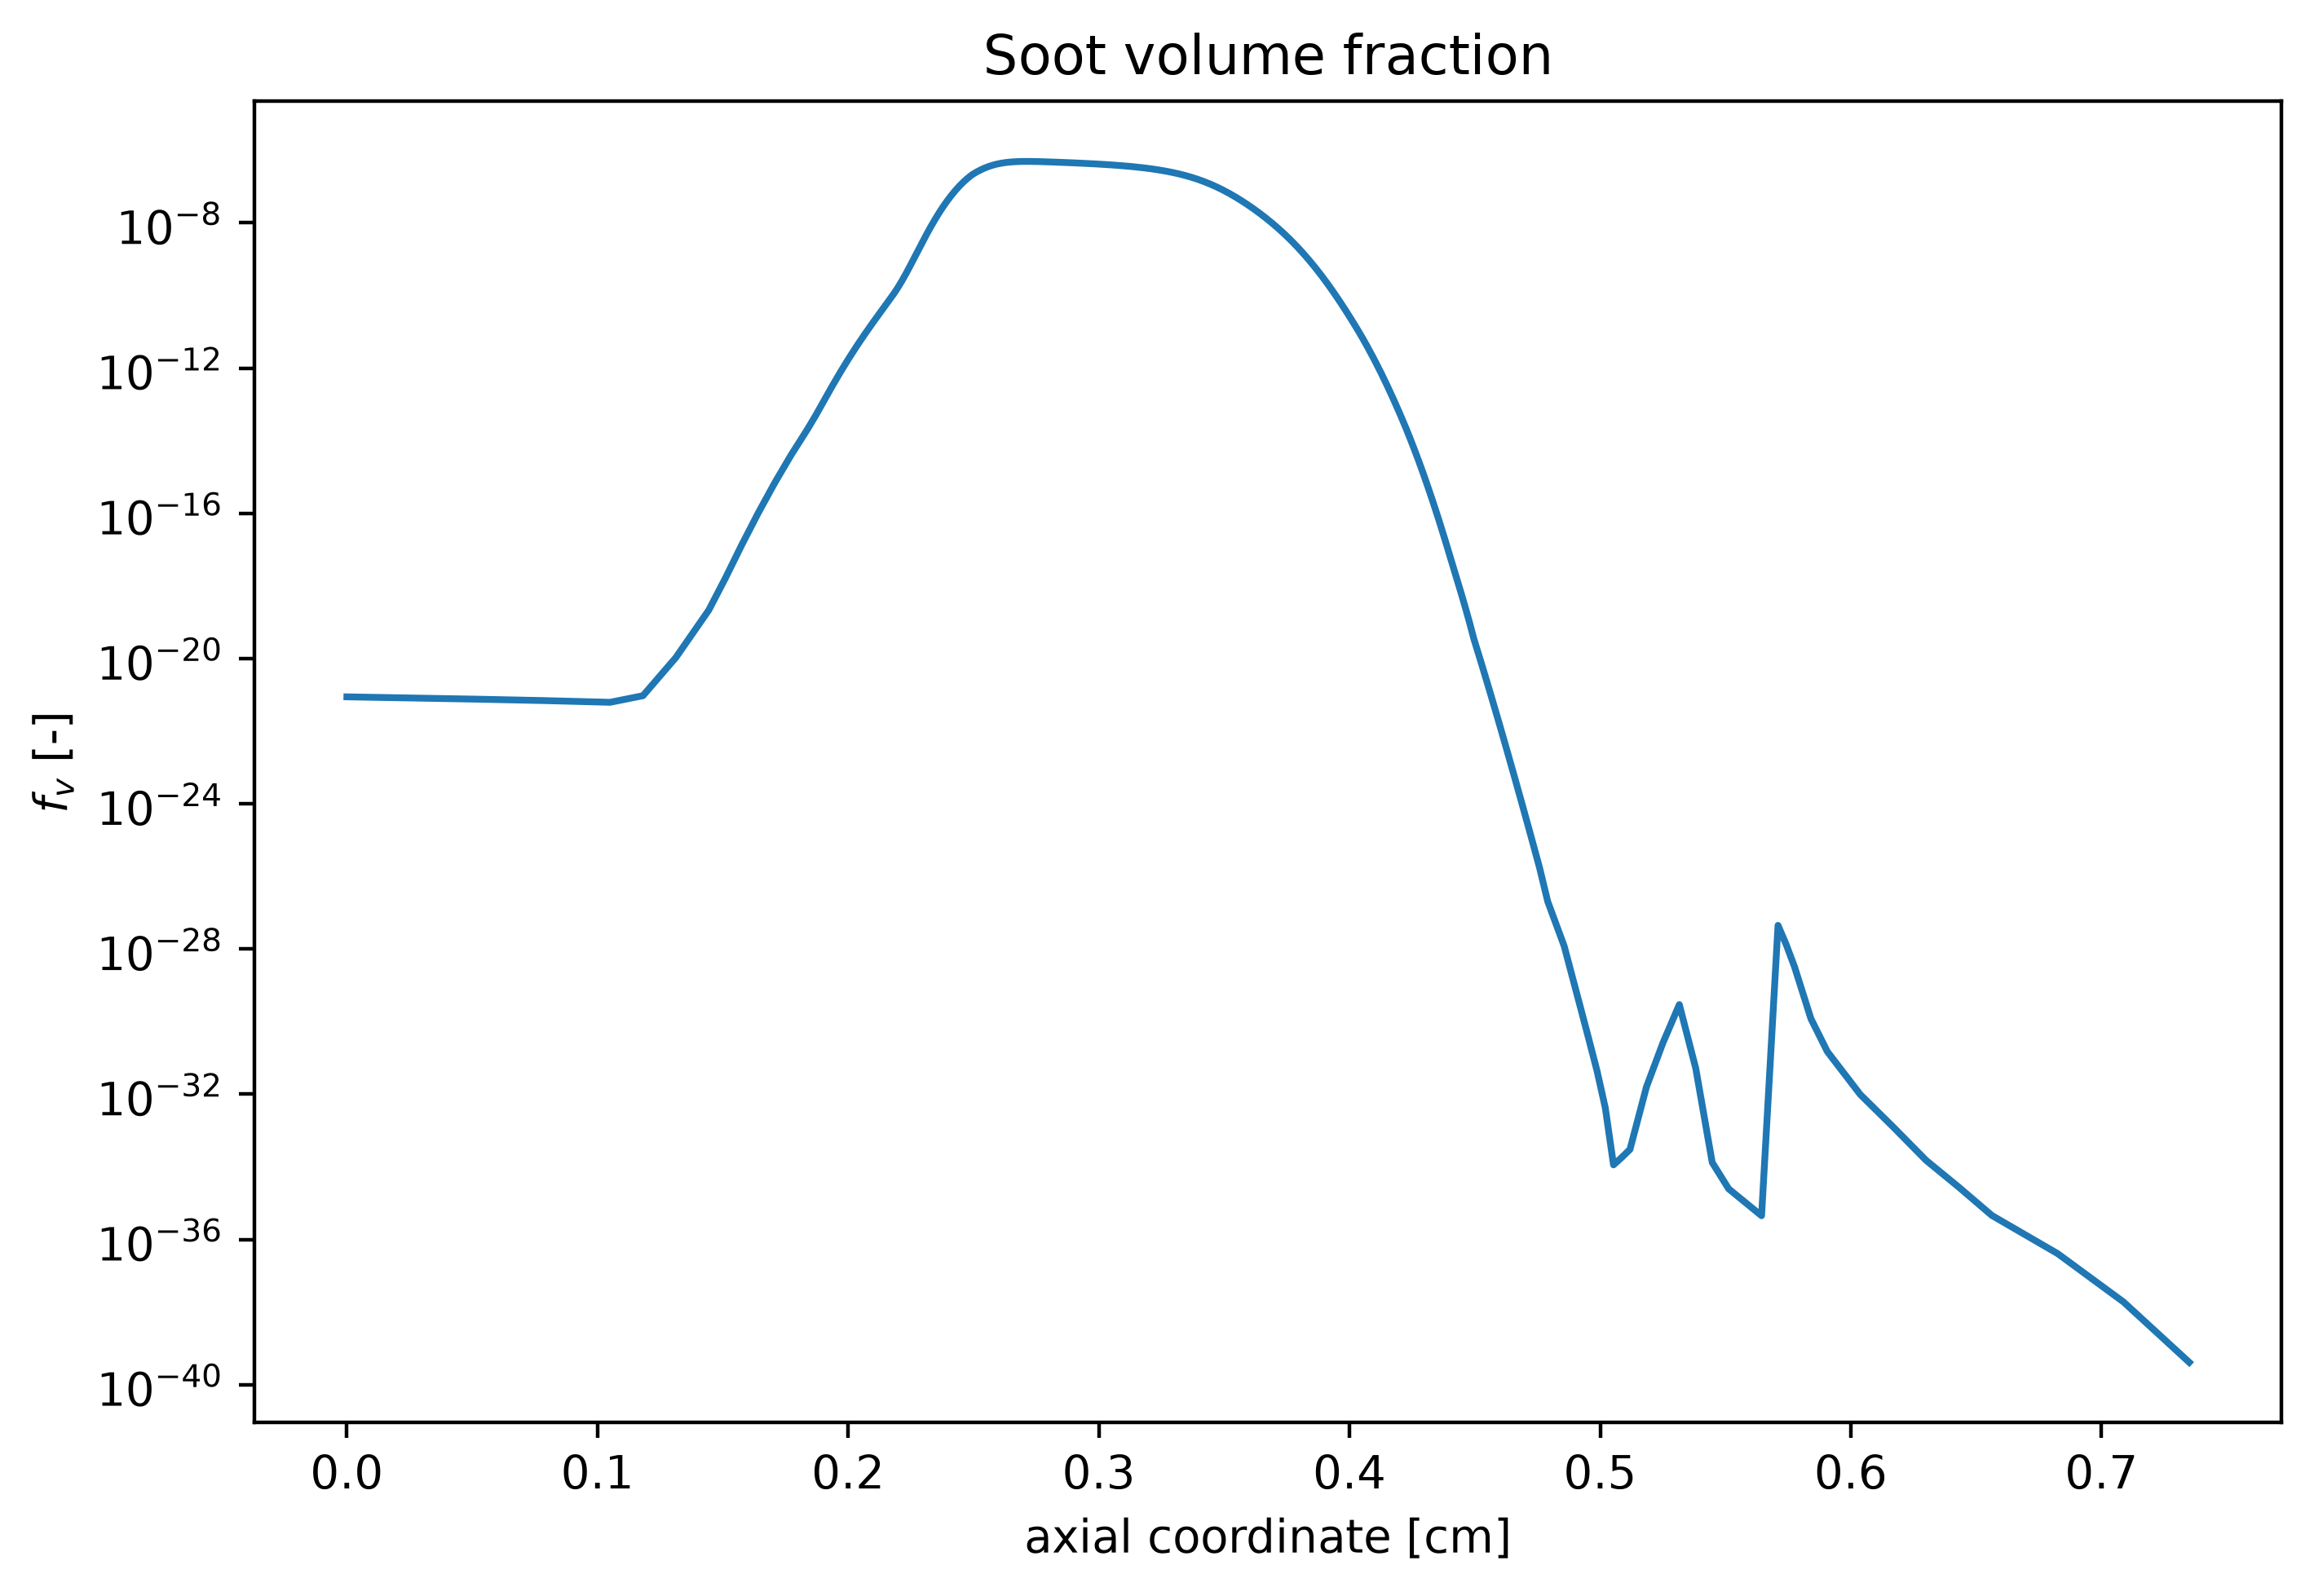
\includegraphics[width=0.75\textwidth]{figures/soot_fv.png}
\caption{Soot volume fraction along the abscissa, \texttt{getFvSootProfile} (\texttt{SootFv.py}, Appendix~\ref{app:examples}).}
\end{figure}

\chapter{Reaction-Class Post-Processing}
\label{ch:reaction-classes}

Module \pkg{pySMOKEPostProcessor.reaction\_classes}. Available when the
mechanism's \pkg{kinetics.xml} (or \pkg{kinetics.surface.xml}) contains a
\pkg{<ReactionClasses>} block, plus a plain-text "class groups" file that
defines how the mechanism's raw subclasses roll up into user-facing groups
(see e.g.\ \pkg{examples/data/Surface\_Data/surf\_rxn\_class.txt}).

This module's \pkg{assignclass} function and \pkg{FluxByClass} class are the
internal machinery that reads a mechanism's \pkg{<ReactionClasses>} block and aggregates ROPA results onto it; every example and notebook in this
guide reaches them only through \pkg{script\_utils.get\_sortedrxns} and
\pkg{script\_utils.process\_classes} (Chapter~\ref{ch:orchestration}), which
is the recommended entry point --- see their source (or docstrings) if you
need to build a custom computation on top of the same machinery. The two functions below, by contrast, \emph{are} meant to be called directly once
you already have the per-simulation flux tables \pkg{process\_classes}
returns.

\pyfunc{merge\_maps\_byspecies(sorted\_dfs\_dct, tosum=False) -> pandas.DataFrame}

Combines the per-simulation heatmap \pkg{DataFrame}s produced by
\pkg{sort\_and\_filter} (one per simulation, same species set) into a single
\pkg{DataFrame}.

\begin{params}
\item \pkg{sorted\_dfs\_dct} (\textit{dict}) --- \pkg{\{simulation\_name:
  DataFrame\}}.
\item \pkg{tosum} (\textit{bool}) --- \pkg{False}: stack rows, renaming each
  species by its simulation (\pkg{"species-simname"}); \pkg{True}: sum
  fluxes for matching species across simulations instead of stacking.
\end{params}
\returns combined \pkg{DataFrame}.

\pyfunc{FDI(sorted\_dfs\_dct, fditype="global", speciesi="", classj="") -> pandas.DataFrame}

Computes pairwise Flux Diagnostic Indices (FDI) between a set of
simulations' class-flux maps. %, following \href{https://doi.org/10.1016/j.combustflame.2022.112073}{Pratali Maffei et al., Combustion and Flame 2022}. % Link a un articolo di Andrea, ma non penso venga di qui in ogni caso.

\begin{params}
\item \pkg{sorted\_dfs\_dct} (\textit{dict}) --- \pkg{\{simulation\_name:
  DataFrame\}} of class fluxes (same shape as for
  \pkg{merge\_maps\_byspecies}).
\item \pkg{fditype} (\textit{str}) --- \pkg{"global"} (sum over all
  species/classes), \pkg{"species"} (sum over classes, for one species) or
  \pkg{"class"} (sum over species, for one class).
\item \pkg{speciesi} (\textit{str}) --- species name, required for
  \pkg{fditype="species"}.
\item \pkg{classj} (\textit{str}) --- class name, required for
  \pkg{fditype="class"}.
\end{params}
\returns square \pkg{DataFrame} (index/columns = simulation names), lower
triangle populated with FDI values (mean-centered), suitable for a heatmap.

\chapter{High-Level Orchestration}
\label{ch:orchestration}

Module \pkg{pySMOKEPostProcessor.script\_utils}. These functions wire
together a \pkg{PostProcessor} and the reaction-class computations of
Chapter~\ref{ch:reaction-classes} for common multi-species / multi-simulation
workflows, and are the recommended entry point for reaction-class analysis.

\pyfunc{get\_sortedrxns(pp, class\_groups\_file, heterogeneous\_reactions=False)}

Classifies the mechanism's reactions from its \pkg{<ReactionClasses>} block
against the class-groups file, returning only the sorted/grouped object.

\begin{params}
\item \pkg{pp} (\textit{PostProcessor}).
\item \pkg{class\_groups\_file} (\textit{str}).
\item \pkg{heterogeneous\_reactions} (\textit{bool}).
\end{params}
\returns the \pkg{rxns\_sorted} object (input to \pkg{process\_classes} and
\pkg{reactionrates\_byclasses} below).

\pyfunc{process\_classes(simul\_fld, kin\_xml\_fld, rxns\_sorted\_obj, species\_list, \\ sortlists, ropa\_type, n\_of\_rxns=100, filter\_dcts=None, threshs=None, \\ weigh="normbyspecies", local\_value=0.0, upper\_value=0.0, lower\_value=0.0, mass\_ropa=False, heterogeneous\_reactions=False, pp=None) -> list[pandas.DataFrame]}

Runs a ROPA for every species in \pkg{species\_list} and groups the combined
flux by reaction class, once per entry of \pkg{sortlists}.

\begin{params}
\item \pkg{simul\_fld}, \pkg{kin\_xml\_fld} (\textit{str}) --- output/kinetics
  folders, used only to build a \pkg{PostProcessor} if \pkg{pp} is not
  given.
\item \pkg{rxns\_sorted\_obj} --- result of \pkg{get\_sortedrxns}.
\item \pkg{species\_list} (\textit{list}) --- either species names
  (\textit{str}) or \pkg{\{combined\_name: [species, ...]\}} dicts to lump
  several species under one combined flux column.
\item \pkg{sortlists} (\textit{list[list[str]]}) --- one grouping-criteria
  list per output \pkg{DataFrame} requested.
\item \pkg{ropa\_type} (\textit{str}) --- \pkg{"global"}, \pkg{"local"} or
  \pkg{"region"}, forwarded to the ROPA calls.
\item \pkg{n\_of\_rxns} (\textit{int}) --- reactions kept per ROPA call.
\item \pkg{filter\_dcts} (\textit{list[dict]}, optional) --- one filter dict
  per \pkg{sortlists} entry.
\item \pkg{threshs} (\textit{list[float]}, optional) --- one threshold per
  \pkg{sortlists} entry (default \pkg{1e-3} each).
\item \pkg{weigh} (\textit{str}).
\item \pkg{local\_value}, \pkg{upper\_value}, \pkg{lower\_value}
  (\textit{float}) --- forwarded to the ROPA calls.
\item \pkg{mass\_ropa} (\textit{bool}).
\item \pkg{heterogeneous\_reactions} (\textit{bool}).
\item \pkg{pp} (\textit{PostProcessor}, optional) --- reuse an existing
  \pkg{PostProcessor} instead of building a fresh one; \textbf{strongly
  recommended} in any loop over timesteps or simulations (re-building
  re-parses \pkg{kinetics.xml}/\pkg{Output.xml} every call).
\end{params}
\returns \textit{list[DataFrame]}, one grouped-flux table per entry of
\pkg{sortlists}, each heatmap-ready (Chapter~\ref{ch:plotting}).

\begin{figure}[h]
\centering
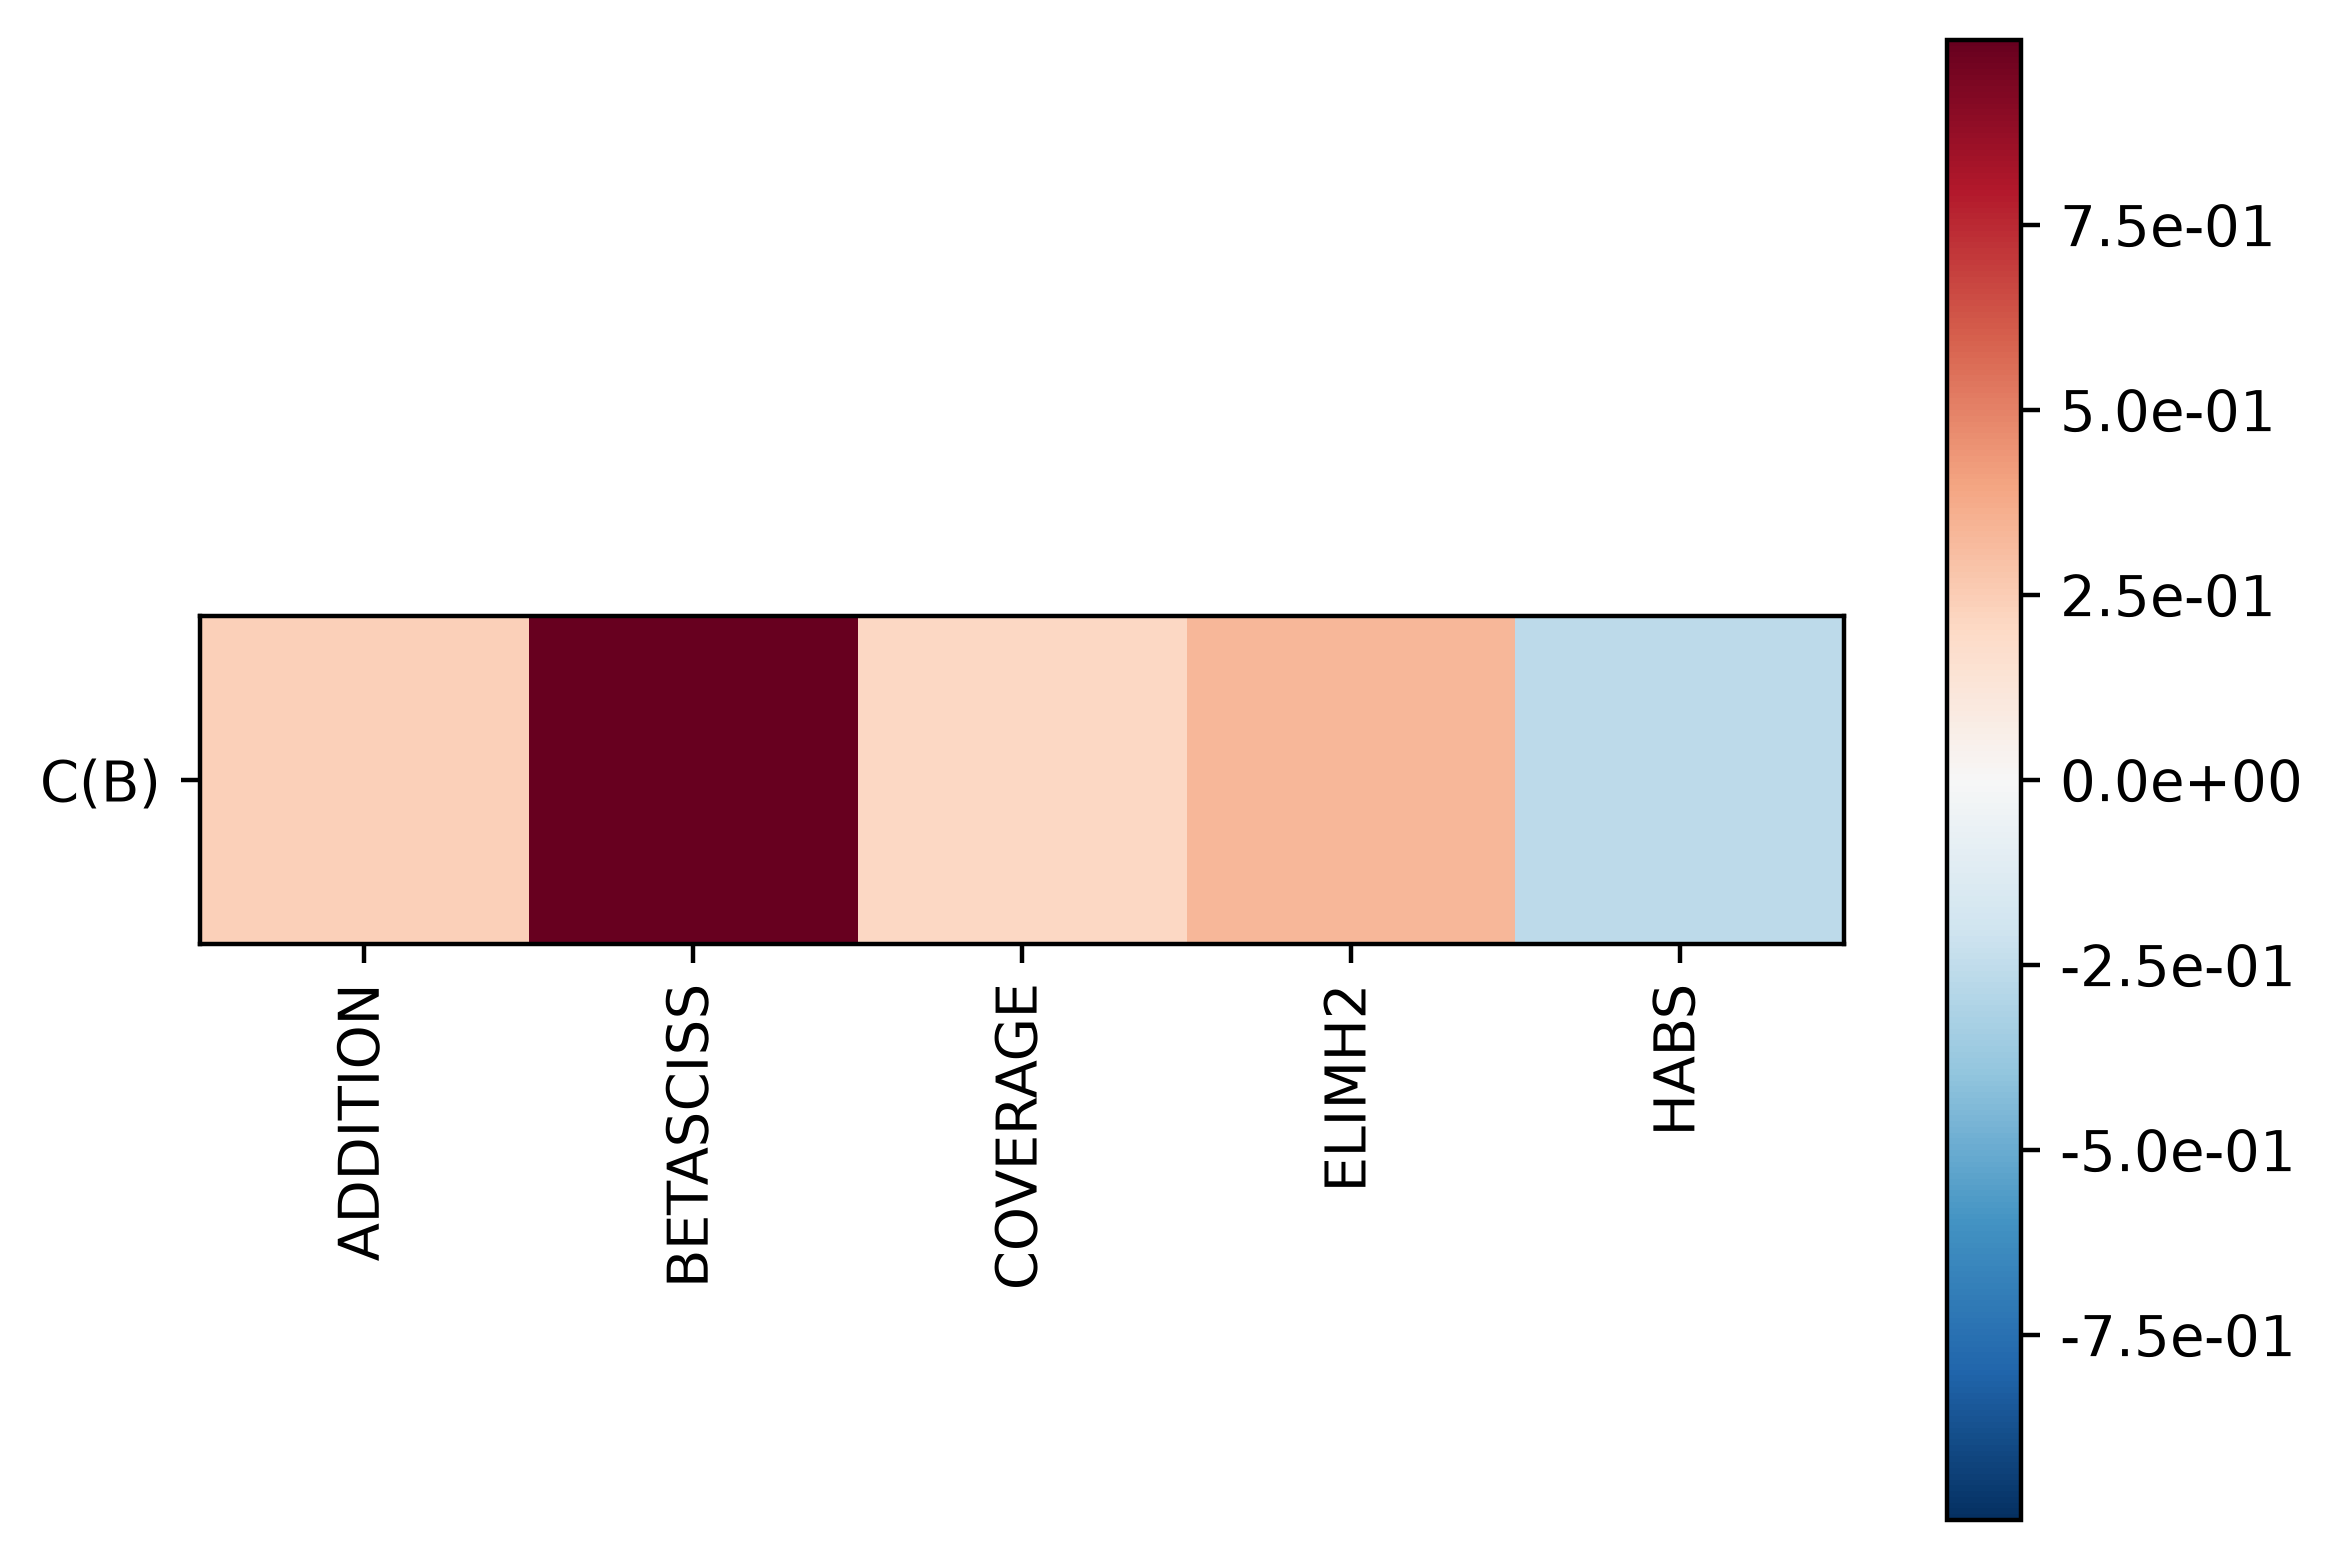
\includegraphics[width=0.6\textwidth]{figures/ropa_by_class_heatmap.png}
\caption{Global ROPA on C(B) grouped by reaction class, for a coupled gas+surface mechanism (\texttt{process\_classes} + \texttt{plot\_heatmap}).}
\label{fig:ropa-by-class-heatmap}
\end{figure}

\pyfunc{cumulative\_rates(simul\_fld, kin\_xml\_fld, species\_list, rate\_type, x\_axis, n\_of\_rxns=100, mass\_ropa=False, threshold=0.01, heterogeneous\_reactions=False, pp=None) -> dict}

Per-species cumulative (time/coordinate-resolved) reaction-rate tables,
built from a global ROPA per species, expanded into full rate profiles and
filtered by cumulative contribution.

\begin{params}
\item \pkg{species\_list} (\textit{list[str]}).
\item \pkg{rate\_type} (\textit{str}) --- \pkg{"PC"} (net), \pkg{"P"}
  (production only) or \pkg{"C"} (consumption only).
\item \pkg{x\_axis} --- kept for signature compatibility; the actual
  abscissa used is always \pkg{pp.getIndependentVariableProfile()}.
\item \pkg{n\_of\_rxns}, \pkg{mass\_ropa}, \pkg{threshold},
  \pkg{heterogeneous\_reactions}, \pkg{pp} --- as in \pkg{process\_classes}.
\end{params}
\returns \pkg{dict} \pkg{\{species: DataFrame\}}, each \pkg{DataFrame}
indexed by the independent variable, columns = individual reactions
(labelled with their \% cumulative contribution), ready for
\pkg{plot\_areas}.

\begin{lstlisting}[language=Python]
cum = script_utils.cumulative_rates(resultsFolder, kineticFolder, species_list=["H2"],
                                     rate_type="PC", x_axis=None, threshold=0.02, pp=pp)
fig, ax = plot_areas(cum["H2"], xlabel="time [s]", ylabel="rate [kmol/m3s]")
\end{lstlisting}

\begin{figure}[h]
\centering
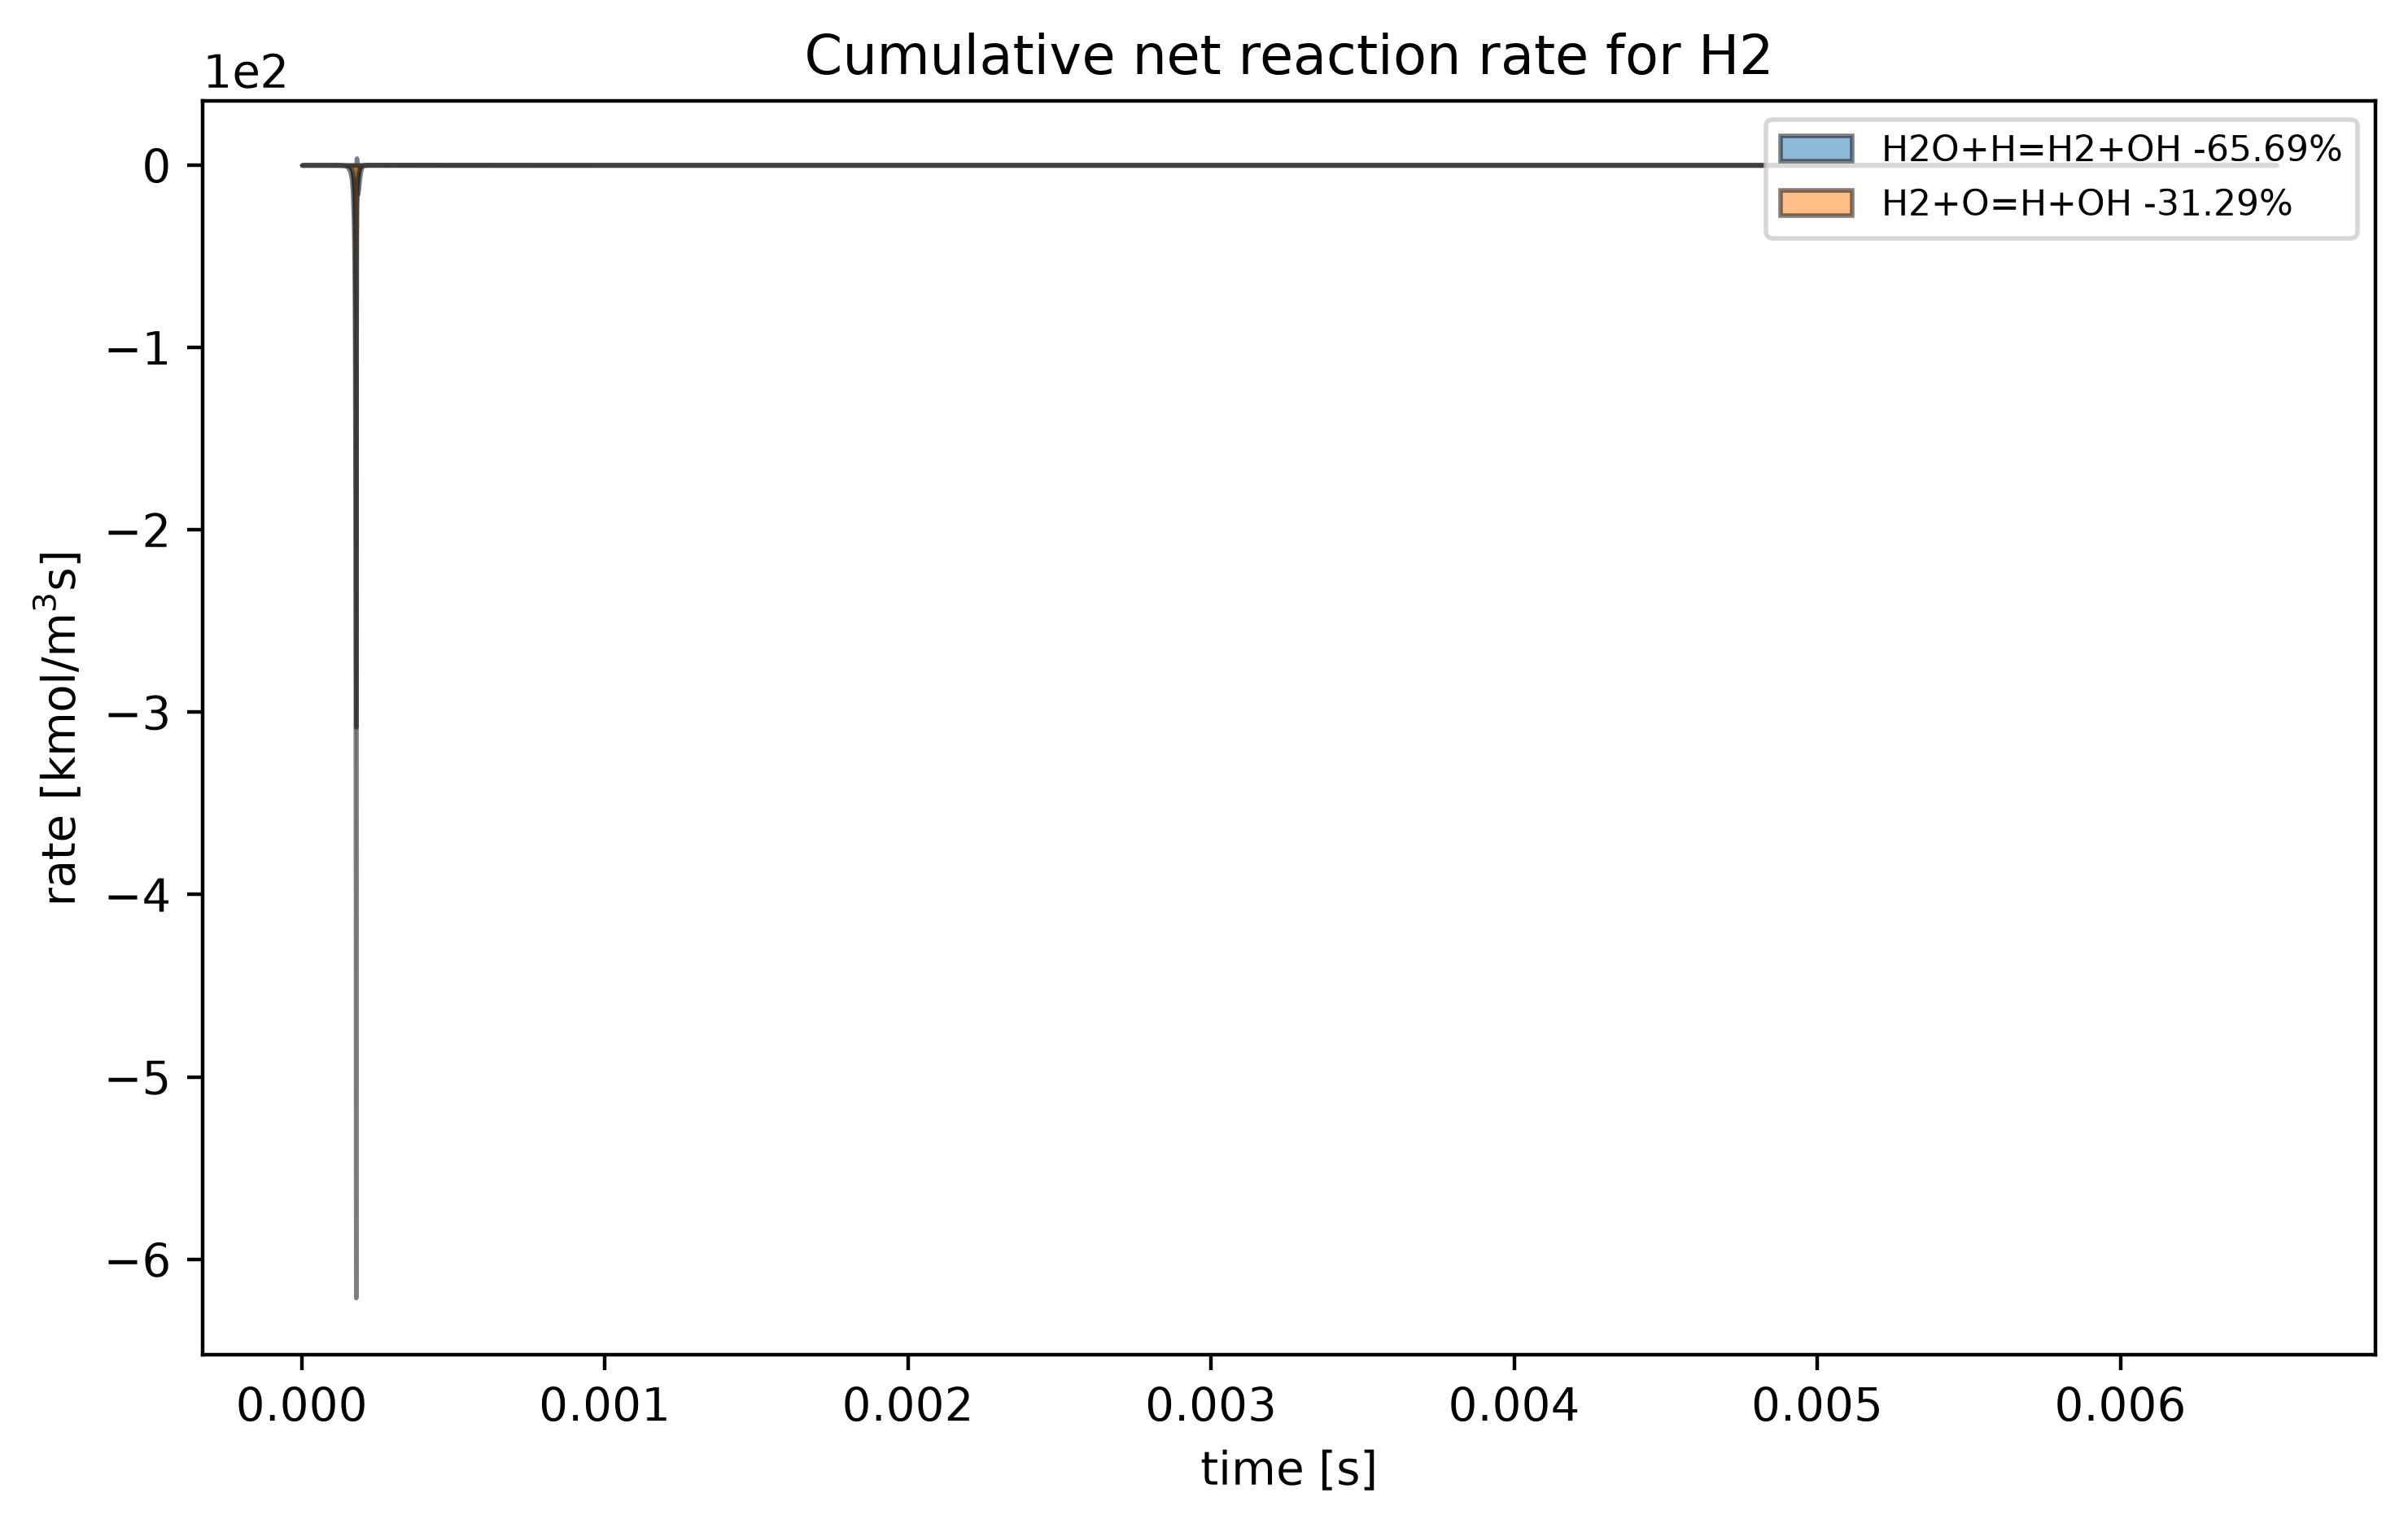
\includegraphics[width=0.75\textwidth]{figures/cumulative_rates_area.png}
\caption{Net (\texttt{"PC"}) cumulative reaction rate for H2 over time, one shaded band per contributing reaction, via \texttt{cumulative\_rates} + \texttt{plot\_areas}.}
\end{figure}

\pyfunc{reactionrates\_byclasses(simul\_fld, kin\_xml\_fld, rxns\_sorted\_df, sortlists, x\_axis, filter\_by\_species=[], filter\_dcts=None, threshs=None, mass\_ropa=False, heterogeneous\_reactions=False, pp=None) -> list[pandas.DataFrame]}

Time/coordinate-resolved reaction rates, summed within each reaction-class
group.

\begin{params}
\item \pkg{rxns\_sorted\_df} --- result of \pkg{get\_sortedrxns}.
\item \pkg{sortlists} (\textit{list[list[str]]}).
\item \pkg{x\_axis} --- see the note in \pkg{cumulative\_rates}.
\item \pkg{filter\_by\_species} (\textit{list[str]}) --- if non-empty,
  restrict to reactions that appear in the global ROPA of these species.
\item \pkg{filter\_dcts}, \pkg{threshs}, \pkg{mass\_ropa},
  \pkg{heterogeneous\_reactions}, \pkg{pp} --- as above.
\end{params}
\returns \textit{list[DataFrame]}, one per \pkg{sortlists} entry, indexed by
the independent variable, columns = class groups, ready for
\pkg{plot\_areas}.

\pkg{cumulative\_rates} and \pkg{reactionrates\_byclasses} are themselves
thin wrappers around \pkg{PostProcessor.cumulativerates} and
\pkg{PostProcessor.reactionrategroups} respectively --- lower-level methods
that operate on an already-computed ROPA result / reaction-name grouping
rather than a class-groups file; reach for them directly only if you are
building a custom grouping outside the reaction-class machinery above (see
their docstrings on \pkg{PostProcessor} for the full signature).

\chapter{Plotting utilities}
\label{ch:plotting}

Module \pkg{pySMOKEPostProcessor.plotting\_utilities}. Thin matplotlib
wrappers around the dict/DataFrame outputs of the analysis methods above.
All take/return standard matplotlib \pkg{Figure}/\pkg{Axes} objects, so the
result can always be customized further with ordinary matplotlib calls.

\pyfunc{plot\_bars(data, ax=None, font=None) -> (Figure, Axes)}

Horizontal bar chart for a ROPA or sensitivity \pkg{dict}. Red bars =
positive coefficients, blue = negative; each bar is labelled with its
reaction name and coefficient value.

\begin{params}
\item \pkg{data} (\textit{dict}) --- a ROPA/sensitivity result dict
  (\pkg{"coefficients"}, \pkg{"reaction\_names"}).
\item \pkg{ax} (\textit{matplotlib.axes.Axes}, optional) --- draw into an
  existing axes instead of creating a new figure.
\item \pkg{font} (\textit{float}, optional) --- label font size; auto-picked
  from the number of bars if omitted.
\end{params}

\pyfunc{plot\_bars\_multiSimulation(data\_list, ax\_list=None, cols=None, rows=None) -> (Figure, list[Axes])}

Draws \pkg{plot\_bars} into a grid of subplots, one per entry of
\pkg{data\_list} (which may itself be a nested list-of-lists to fix the grid
shape).

\begin{params}
\item \pkg{data\_list} --- flat or nested list of ROPA/sensitivity dicts.
\item \pkg{ax\_list} (\textit{list[Axes]}, optional) --- reuse an existing
  grid.
\item \pkg{cols}, \pkg{rows} (\textit{int}, optional) --- grid shape, if not
  inferable from a nested \pkg{data\_list}.
\end{params}

\pyfunc{plot\_heatmap(sort\_df, symmetricaxis=False, dftype="generic", compressratio=1) -> Figure}

Heatmap of a grouped-flux \pkg{DataFrame} (as returned by
\pkg{script\_utils.process\_classes}), with a diverging (red/blue,
zero-centered) colormap.

\begin{params}
\item \pkg{sort\_df} (\textit{DataFrame}) --- rows/columns become the
  heatmap's y/x axes.
\item \pkg{symmetricaxis} (\textit{bool}) --- force a symmetric color scale
  around zero (else the scale is shifted so zero maps to its data-driven
  position).
\item \pkg{dftype} (\textit{str}) --- \pkg{"generic"} (use row labels as-is)
  or \pkg{"flux"} (strip a leading \pkg{"flux\_"} from row labels).
\item \pkg{compressratio} (\textit{float}) --- compress the plot's aspect
  ratio (useful for very tall/wide tables).
\end{params}

\pyfunc{plot\_class\_distribution(data\_df, xlabel="coordinate", ylabel="element fraction", title="", colors=None, fontsize=8, loc="upper right", edgecolor="k", linewidth=0.4, alpha=1.0, reverse\_legend=True) -> (Figure, Axes)}

Stacked-area plot for a per-class distribution (e.g.\ the output of
\pkg{ElementalDistributionByClass}) --- one filled band per class.

\begin{params}
\item \pkg{data\_df} (\textit{DataFrame}) --- index = independent variable,
  one column per class.
\item \pkg{colors} (\textit{list}, optional) --- defaults to seaborn
  "muted" if seaborn is installed, else the matplotlib \pkg{tab20} cycle.
\item \pkg{reverse\_legend} (\textit{bool}) --- order the legend to match
  the visible top-to-bottom stacking order.
\item (remaining parameters are standard matplotlib cosmetics.)
\end{params}

\pyfunc{plot\_areas(data\_df, xlabel="x axis", ylabel="y axis", title="", fontsize="8", loc="upper right", plotlines=False) -> (Figure, Axes)}

Shaded-area (or, with \pkg{plotlines=True}, plain line) plot for a
multi-column \pkg{DataFrame}, e.g.\ the output of \pkg{cumulative\_rates}/
\pkg{reactionrates\_byclasses}.

\begin{params}
\item \pkg{data\_df} (\textit{DataFrame}) --- index = x-axis, one column per
  series.
\item \pkg{plotlines} (\textit{bool}) --- draw lines instead of stacked
  shaded areas.
\item (remaining parameters are standard matplotlib cosmetics.)
\end{params}

\pyfunc{plot\_distribution(df, ax=None, label=None, **plot\_kw) -> Axes}

Line plot of $dN/d\log_{10}(d)$ vs.\ particle diameter $d$ (log y-axis) for
a \pkg{SootPSD} \pkg{DataFrame}.

\begin{params}
\item \pkg{df} (\textit{DataFrame}) --- a \pkg{PostProcessor.SootPSD} result.
\item \pkg{ax} (\textit{Axes}, optional).
\item \pkg{label} (\textit{str}, optional) --- defaults to
  \pkg{"abscissa = ..."}.
\item \pkg{**plot\_kw} --- forwarded to \pkg{Axes.plot} (e.g.\
  \pkg{marker}, \pkg{linestyle}).
\end{params}

The module also has \pkg{plot\_multiple\_bars} (a grouped-bar-chart variant
of \pkg{plot\_bars} for several parallel series) and \pkg{save\_fig} (batch-save
a figure under a class-list-derived filename); neither is exercised by any
bundled example, so see their docstrings in \pkg{plotting\_utilities/} if you
need them.

\chapter{Element speciation utility}

\pyfunc{elements\_balance(kineticFolder, resultsFolder, elements\_list, threshold=0.05)}

Module \pkg{pySMOKEPostProcessor.elements\_balance}. Plots, for each element
requested, a stackplot of which species carries it across a run --- a
higher-level convenience on top of \pkg{ElementMolesBySpecies} that also
handles temperature-sweep result layouts.

\begin{params}
\item \pkg{kineticFolder} (\textit{str}) --- folder containing
  \pkg{kinetics.xml}.
\item \pkg{resultsFolder} (\textit{str}) --- either a folder of
  \pkg{Case*/} subfolders (a sweep: one point per case, plotted against that
  case's final temperature) or a single run's output folder (every point of
  its own independent variable is used).
\item \pkg{elements\_list} (\textit{list[str]}) --- element symbols, any
  case accepted (\pkg{"he"}, \pkg{"HE"}, \pkg{"He"} all match); elements
  absent from the mechanism are skipped with a warning.
\item \pkg{threshold} (\textit{float}) --- a species gets its own band if it
  holds more than this fraction of the element's total at some point;
  everything else is lumped into \pkg{"Others"}.
\end{params}
Calls \pkg{plt.show()} internally; does not return a figure handle. If
\pkg{resultsFolder} contains \pkg{Case*/} subfolders (a sweep, e.g.\ over
inlet temperature), one steady-state point per case is plotted against that
case's final temperature instead of the run's own independent variable ---
the function auto-detects which mode applies by checking for \pkg{Case*}
subfolders.

\begin{lstlisting}[language=Python]
from pySMOKEPostProcessor import elements_balance

elements_balance(kineticFolder, resultsFolder, elements_list=["C", "H", "O"],
                  threshold=0.05)
\end{lstlisting}

\begin{figure}[h]
\centering
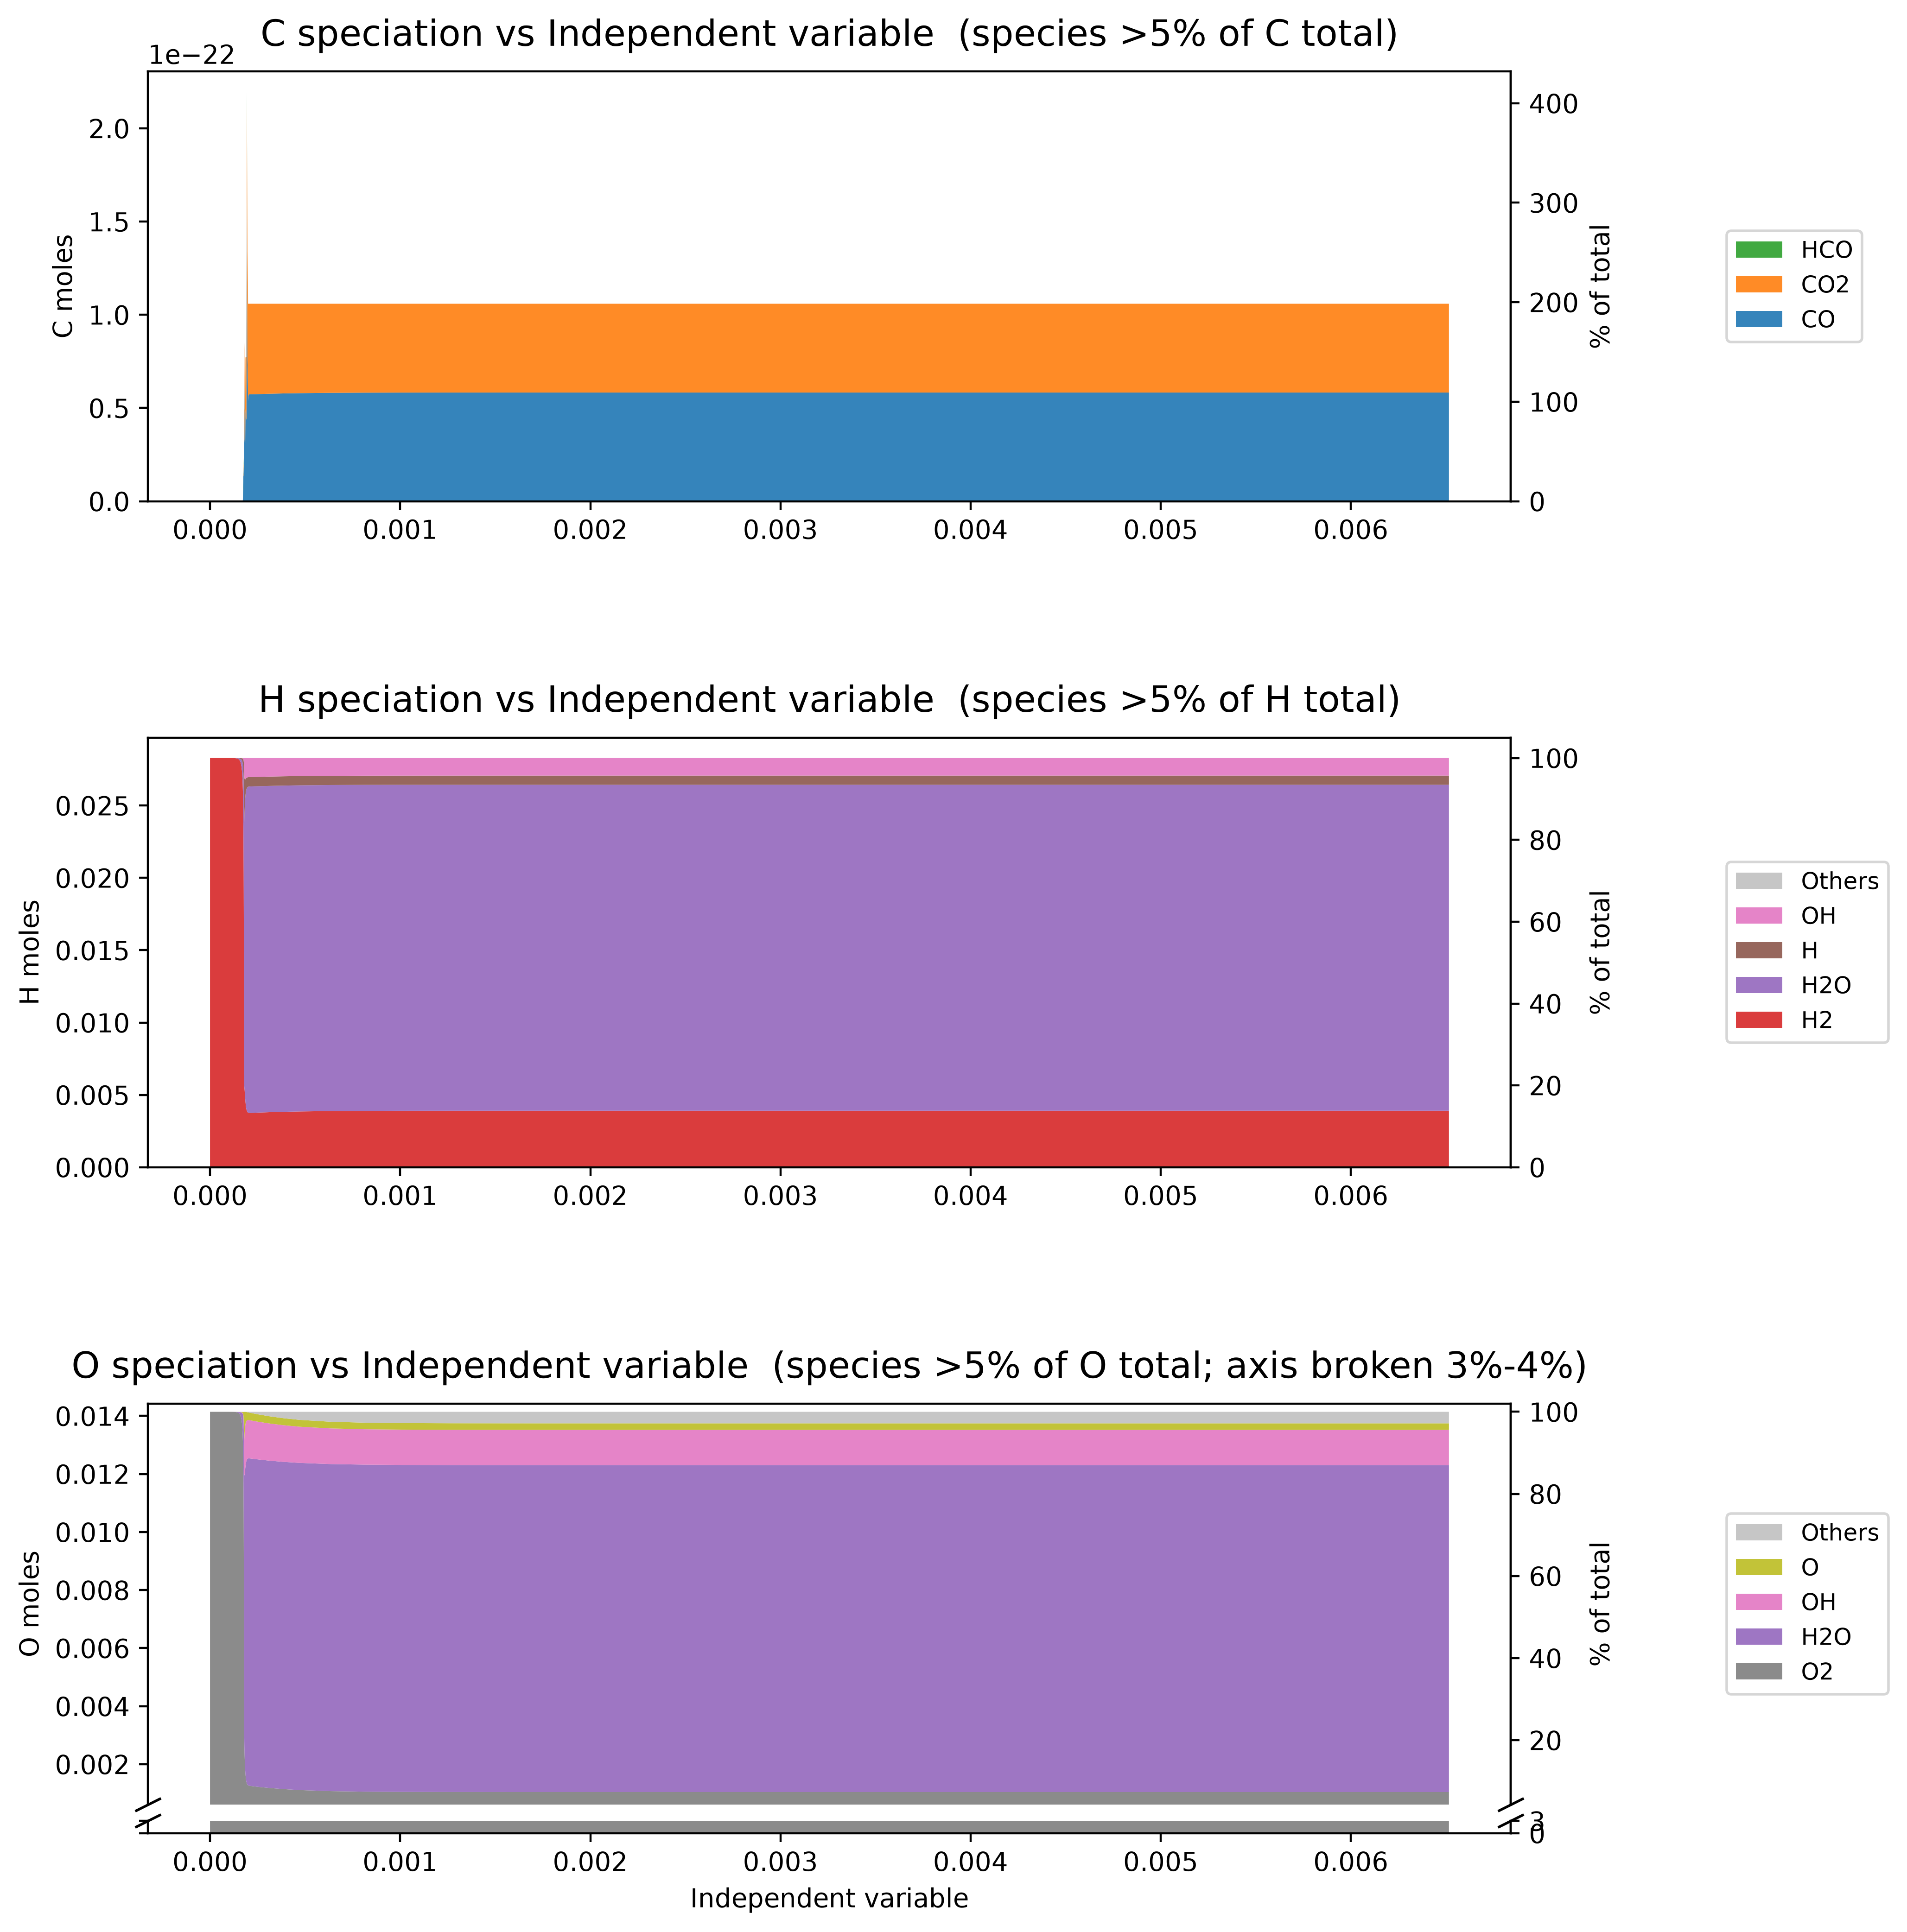
\includegraphics[width=\textwidth]{figures/elements_balance.png}
\caption{Element speciation for C, H and O across a single run, one stacked panel per element; species below the 5\% threshold are lumped into "Others". Note the broken y-axis automatically inserted on the O panel when a single species (here O2) otherwise dominates the plot.}
\end{figure}

\chapter{Surface-reactions utilities}

Module \pkg{pySMOKEPostProcessor.surfacereactions\_utilities}. Domain-specific
helpers for coupled gas+surface (deposition) mechanisms: running a
reaction-class ROPA at every simulation timestep, time-integrating it, and
stack-plotting the cumulative result.

\pyclass{CumulativeROPAByClass}

Shared parent class of \pkg{CumulativeDeposition} and
\pkg{CumulativeSootProduction} below; not normally instantiated directly.
Both subclasses run a local (per-timestep) ROPA-by-class over the whole
simulation for a fixed set of target species, collapse those species onto
one combined row per timestep, time-integrate the result, and stack-plot it
by reaction class.

\pyclass{CumulativeDeposition}

\pymethod{CumulativeDeposition(kineticFolder, outputFolder, class\_group\_file, \\ allCarbon=False, sort\_type=[['reactiontype']], carbon\_density=2000.0, area=None)}

\begin{params}
\item \pkg{kineticFolder} (\textit{str}) --- folder containing
  \pkg{kinetics.surface.xml} and \pkg{surface\_reaction\_names.xml}.
\item \pkg{outputFolder} (\textit{str}) --- folder containing
  \pkg{Output.xml}.
\item \pkg{class\_group\_file} (\textit{str}) --- class-groups text file.
\item \pkg{allCarbon} (\textit{bool}) --- evaluate deposition on all bulk
  carbon species (\pkg{True}) or on \pkg{C(B)} only (\pkg{False}).
\item \pkg{sort\_type} (\textit{list[list[str]]}) --- default reaction-class
  grouping.
\item \pkg{carbon\_density} (\textit{float}, kg/m$^3$) --- used for
  thickness conversion.
\item \pkg{area} (\textit{float}, optional) --- deposition area; required
  for extensive (\pkg{"mass"}/\pkg{"moles"}) output units.
\end{params}

\pymethod{plotCumulativeDeposition(profilesTag="profiles", lump\_steps=1,\\  units="mass-specific", threshold=0.01, fig=None, ax=None, colors=seaborn "muted") -> (Figure, Axes)}

\begin{params}
\item \pkg{profilesTag} (\textit{str}) --- tag to look for in
  \pkg{Output.xml}.
\item \pkg{lump\_steps} (\textit{int}) --- subsample the timestep grid by
  this factor (faster, coarser integration).
\item \pkg{units} (\textit{str}) --- \pkg{"mass-specific"},
  \pkg{"moles-specific"}, \pkg{"mass"}, \pkg{"moles"} or \pkg{"thickness"}.
\item \pkg{threshold} (\textit{float}) --- classes below this fraction of
  the peak total are dropped from the plot.
\item \pkg{fig}, \pkg{ax} --- reuse existing matplotlib objects (for
  subplot composition) instead of creating new ones.
\item \pkg{colors} --- color sequence for the stacked classes.
\end{params}
\returns \pkg{(Figure, Axes)} of the stacked-area cumulative-deposition
plot.

\pyclass{CumulativeSootProduction}

\pymethod{CumulativeSootProduction(kineticFolder, outputFolder, class\_group\_file, soot\_species=None, sort\_type=[['reactiontype']], volume=None)}

\begin{params}
\item \pkg{kineticFolder}, \pkg{outputFolder}, \pkg{class\_group\_file},
  \pkg{sort\_type} --- as in \pkg{CumulativeDeposition}.
\item \pkg{soot\_species} (\textit{list[str]}, optional) --- explicit list
  of soot species; if omitted, auto-resolved from the mechanism's
  \pkg{<SpeciesClasses>} \pkg{SOOT*} classes, falling back to a hardcoded
  legacy BIN-name list for pre-2024 mechanisms with no
  \pkg{<SpeciesClasses>} block. Raises \pkg{ValueError} if neither approach
  finds anything.
\item \pkg{volume} (\textit{float}, optional) --- required for the
  extensive \pkg{"mass"} output unit.
\end{params}

\pymethod{plotSootProduction(profilesTag="profiles", lump\_steps=1, units="mass-specific", threshold=0.01, fig=None, ax=None, colors=seaborn "muted") -> (Figure, Axes)}

Same parameters and behaviour as \pkg{plotCumulativeDeposition} above, for
gas-phase soot mass production instead of surface deposition; \pkg{units}
accepts \pkg{"mass-specific"} or \pkg{"mass"} only.

Both classes share the same \pkg{fig}/\pkg{ax} pattern precisely so they can
be composed into one figure, e.g.\ deposited carbon mass against gas-phase
soot mass produced over the same run (as in
\pkg{examples/surfacereactions/DepositionROPA.py}, Appendix~\ref{app:examples}):

\begin{lstlisting}[language=Python]
Bulk = CumulativeDeposition(kineticFolder, outputFolder, surface_classes,
                             sort_type=[["reactiontype"]], area=200./1E4, allCarbon=True)
Soot = CumulativeSootProduction(kineticFolder, outputFolder, gas_classes,
                                 sort_type=[["reactiontype"]], volume=100./1E4)

fig, ax = plt.subplots(2, 1, figsize=(10.5, 12.), sharex=True)
fig, ax[0] = Bulk.plotCumulativeDeposition(lump_steps=4, units="mass", fig=fig, ax=ax[0])
fig, ax[1] = Soot.plotSootProduction(lump_steps=4, units="mass", fig=fig, ax=ax[1])
ax[1].invert_yaxis()  # mirror the soot panel below the deposition panel
\end{lstlisting}

\begin{figure}[h]
\centering
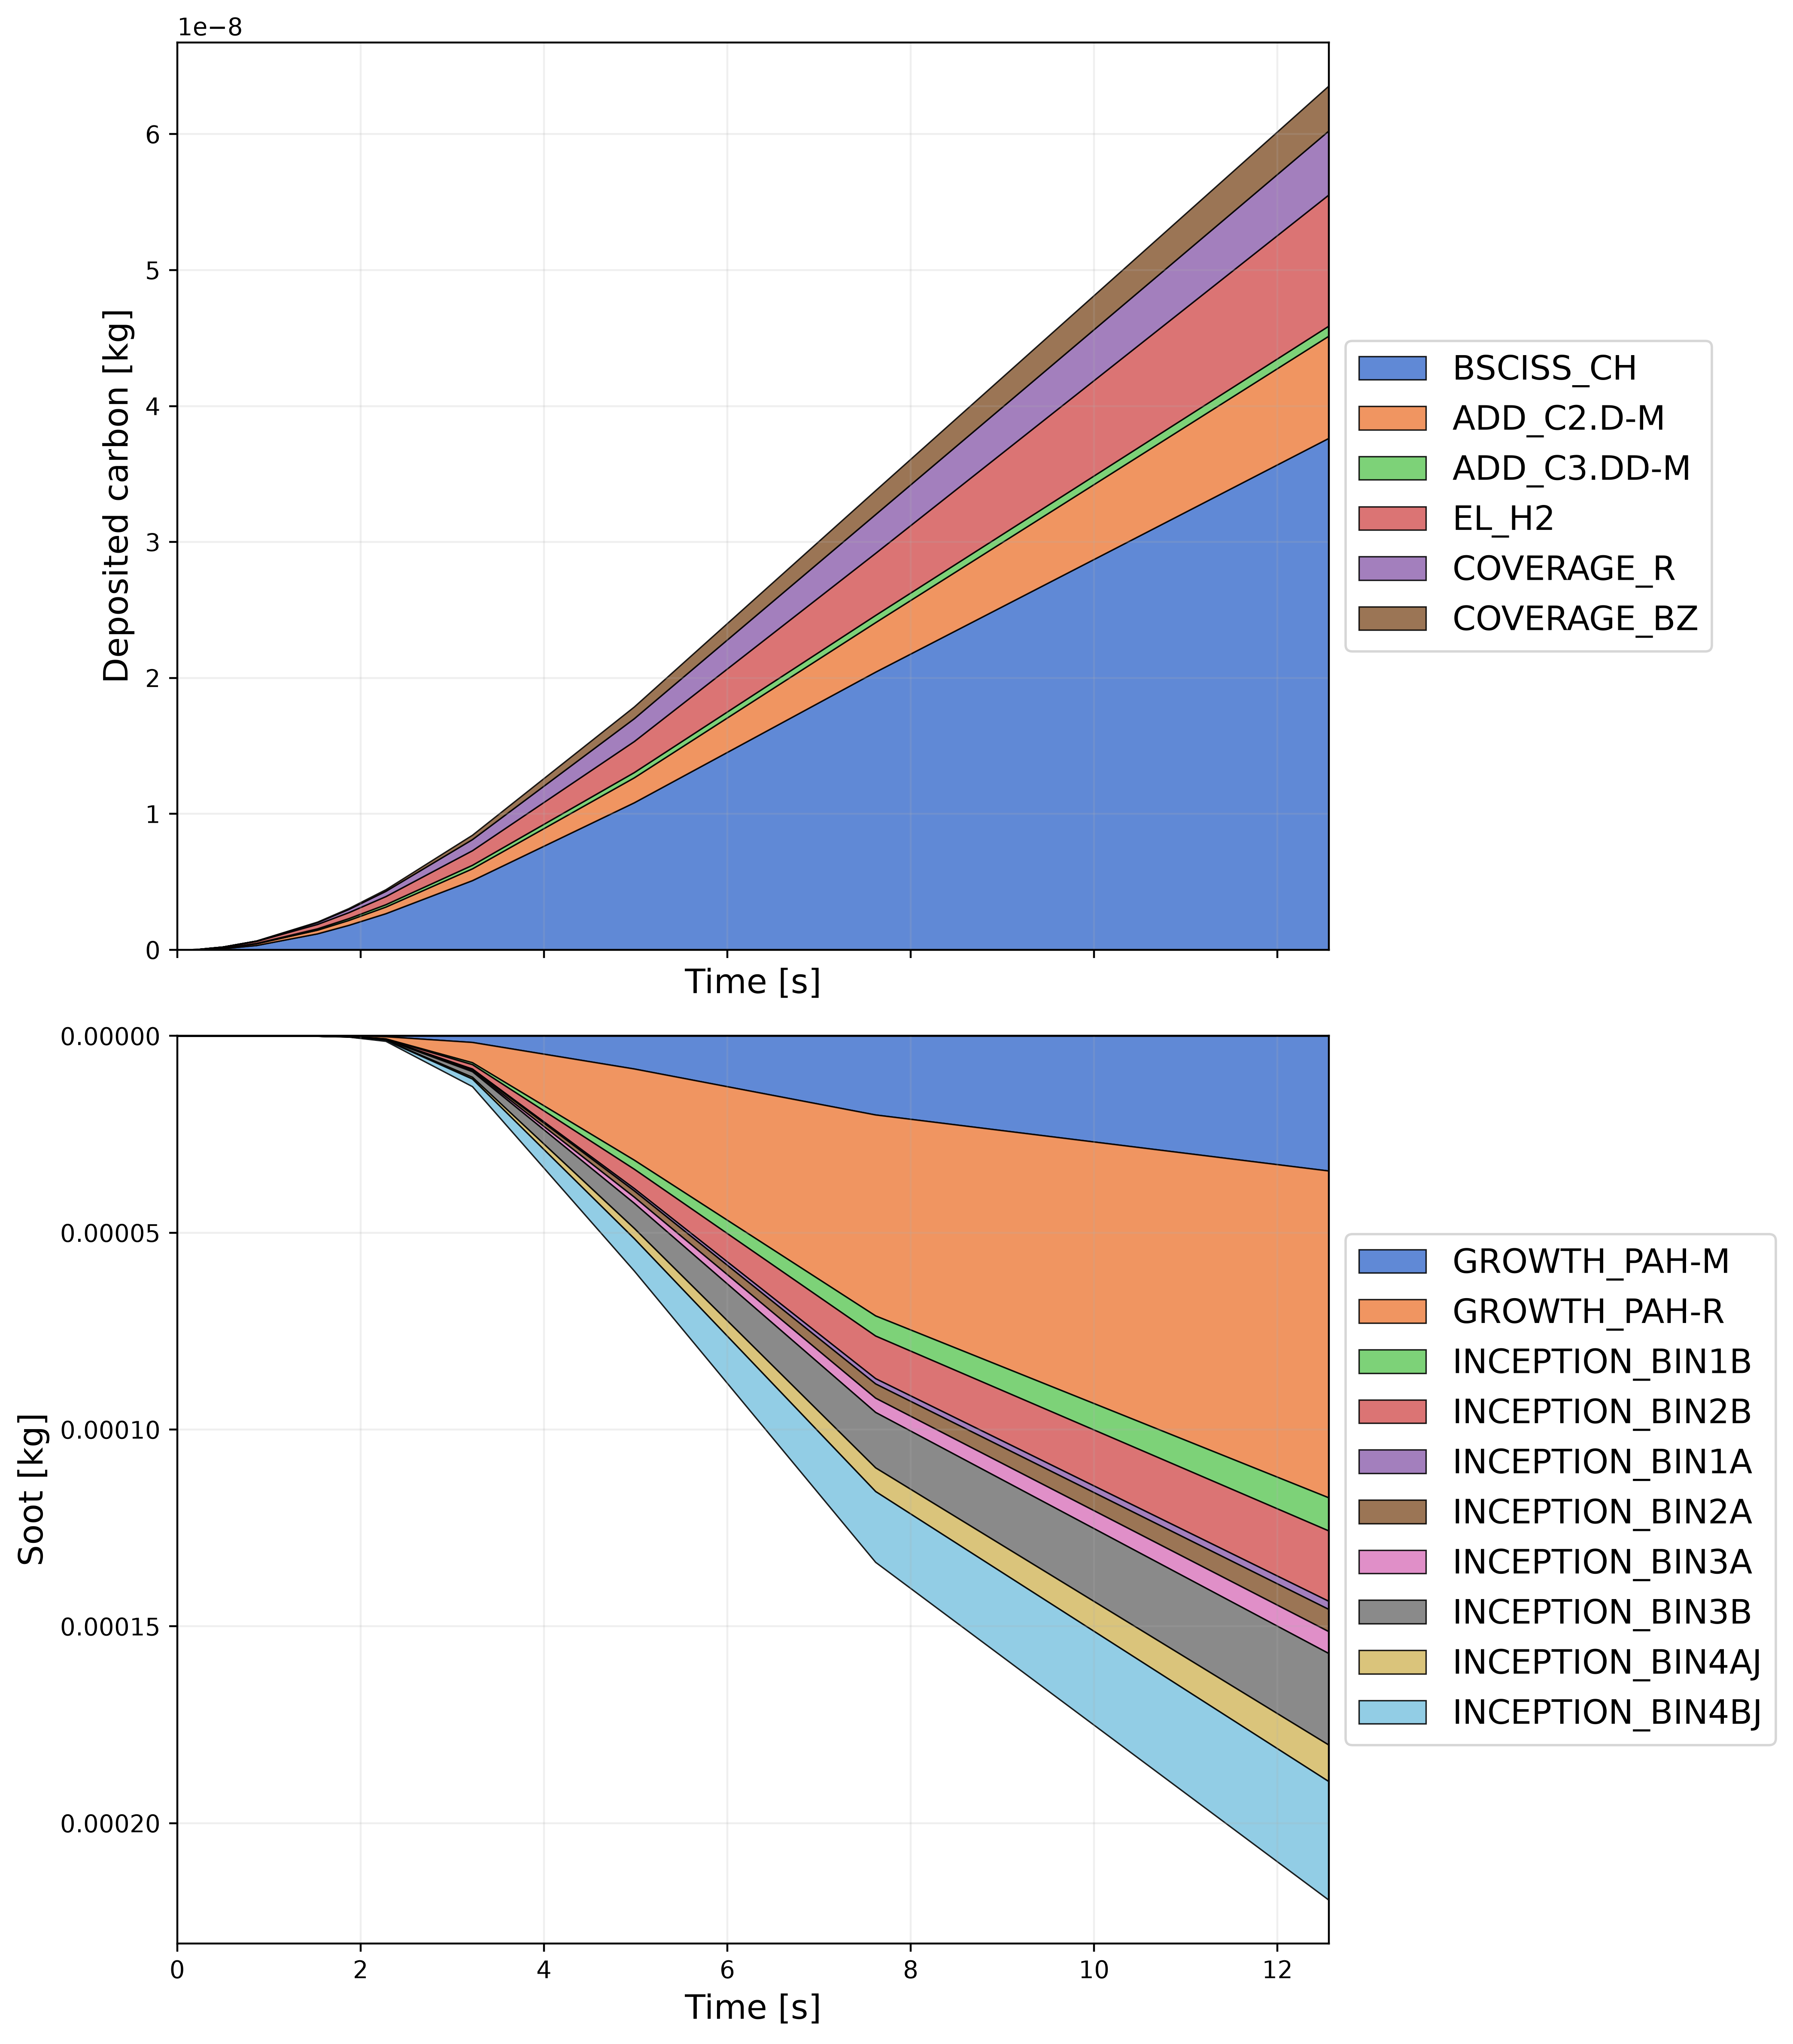
\includegraphics[width=0.72\textwidth]{figures/deposition_soot.png}
\caption{Cumulative deposited carbon mass (top, by surface reaction class) mirrored against cumulative gas-phase soot mass production (bottom, inverted axis, by gas reaction class), sharing a time axis.}
\end{figure}

Internally, both classes read the timestep grid and time-integrate their
per-timestep ROPA table via the module's \pkg{getTimeProfile}/
\pkg{getROPAIntegralTimeHistory} helpers; not normally called directly.

\chapter{\texttt{GraphWriter} (internal helper)}

\pyclass{GraphWriter}

Used internally by \pkg{FluxAnalysis} and \pkg{FluxAnalysisByClass} to turn
a set of (start, end, thickness, label) edges into a
\pkg{graphviz.Digraph}; not normally called directly by user code, but
available at \pkg{pySMOKEPostProcessor.graph\_writer.GraphWriter} for custom
flux-graph construction.

\begin{params}
\item \pkg{GraphWriter(fluxAnalysisType)} --- \pkg{fluxAnalysisType} is
  \pkg{"production"} (blue edges) or \pkg{"destruction"} (red edges).
\item \pkg{CreateGraph(edgeStart, edgeEnd, thickness, label) -> graphviz.Digraph}
  --- builds the graph from four parallel lists (node names, node names,
  edge weights, edge \% labels).
\end{params}

\chapter{Common recipes}
\label{ch:recipes}

Self-contained snippets for patterns that come up repeatedly but are spread
across several chapters above. All assume
\pkg{from pySMOKEPostProcessor import PostProcessor} (and the relevant
plotting import) has already run.

\section{Build once, reuse across many outputs (parameter sweep)}

Any workflow that touches the same mechanism against many \pkg{Output.xml}
folders --- a temperature/pressure sweep, a per-timestep loop --- should
build one \pkg{PostProcessor} and move it with \pkg{updateOutput}, not
reconstruct one per folder. Reconstructing re-parses \pkg{kinetics.xml} (and
re-does the one-off \pkg{<ReactionClasses>}/\pkg{<SpeciesClasses>} scan)
every time, for no benefit once the mechanism is fixed.

\begin{lstlisting}[language=Python]
import glob, os

case_folders = sorted(glob.glob(os.path.join(resultsFolder, "Case*")))
pp = PostProcessor(kineticFolder, case_folders[0])

peak_T = {}
for case_folder in case_folders:
    if case_folder != case_folders[0]:
        pp.updateOutput(case_folder)
    _, T = pp.getTemperatureProfile()
    peak_T[case_folder] = float(T.max())
\end{lstlisting}

The same pattern underlies \pkg{elements\_balance}'s sweep mode
(Chapter~\ref{ch:reaction-classes}'s neighbour) and is why every
orchestration helper in Chapter~\ref{ch:orchestration}
(\pkg{process\_classes}, \pkg{cumulative\_rates}, \pkg{reactionrates\_byclasses})
accepts an optional \pkg{pp=} to reuse an existing \pkg{PostProcessor}
instead of building its own.

\section{Reaction-class analysis, start to finish}

The three-step pattern behind every reaction-class plot in this guide
(Chapters~\ref{ch:reaction-classes}--\ref{ch:orchestration}): classify once,
then run as many ROPA-by-class calls as needed against that classification.

\begin{lstlisting}[language=Python]
from pySMOKEPostProcessor import PostProcessor, script_utils, plot_heatmap

pp = PostProcessor(kineticFolder, outputFolder)

# 1. Classify the mechanism's reactions (reads <ReactionClasses> once)
rxns_sorted = script_utils.get_sortedrxns(pp, class_groups_file,
                                           heterogeneous_reactions=False)

# 2. Run ROPA on the species of interest, grouped by class
sortdfs = script_utils.process_classes(
    outputFolder, kineticFolder, rxns_sorted,
    species_list=["OH", "CH3"], sortlists=[["reactiontype"], ["classtype"]],
    ropa_type="global", n_of_rxns=50, pp=pp)

# 3. Plot
fig_by_reactiontype = plot_heatmap(sortdfs[0], dftype="flux")
fig_by_classtype = plot_heatmap(sortdfs[1], dftype="flux")
\end{lstlisting}

\section{Comparing several simulations with FDI}

Flux Diagnostic Indices (Chapter~\ref{ch:reaction-classes}) quantify how
different two or more simulations' class-flux fingerprints are --- useful to
screen "which of these N cases actually behaves differently" before
digging into any one of them by hand.

\begin{lstlisting}[language=Python]
from pySMOKEPostProcessor import script_utils, reaction_classes as rc

sorted_dfs = {}
for name, (kin, out) in simulations.items():         # {name: (kinFolder, outFolder)}
    pp = PostProcessor(kin, out)
    rxns_sorted = script_utils.get_sortedrxns(pp, class_groups_file)
    sortdfs = script_utils.process_classes(out, kin, rxns_sorted,
                                            species_list=species_list,
                                            sortlists=[["classtype"]],
                                            ropa_type="global", pp=pp)
    sorted_dfs[name] = sortdfs[0]

merged = rc.merge_maps_byspecies(sorted_dfs)   # sanity-check / inspect if needed
fdi = rc.FDI(sorted_dfs, fditype="global")
\end{lstlisting}

\section{Gas + surface (deposition) mechanisms}

Constructing a \pkg{PostProcessor} on a coupled mechanism auto-detects the
surface phase (from \pkg{kinetics.surface.xml}) and sets
\pkg{pp.isHeterogeneous}; ROPA and Sensitivity calls additionally take their
own \pkg{heterogeneous\_reactions}/\pkg{heterogeneous\_sensitivity} flag to
pick which side of the coupled mechanism (gas or surface) the call applies
to:

\begin{lstlisting}[language=Python]
pp = PostProcessor(kineticFolder, outputFolder)   # kinetics.surface.xml auto-detected
assert pp.isHeterogeneous

gas_ropa = pp.RateOfProductionAnalysis("CH4", ropa_type="global",
                                        heterogeneous_reactions=False)
surf_ropa = pp.RateOfProductionAnalysis("C(B)", ropa_type="global",
                                         heterogeneous_reactions=True)
\end{lstlisting}

\section{Notebook display of graphviz results}

\pkg{FluxAnalysis} and \pkg{FluxAnalysisByClass}'s \pkg{"graph"} both return
a \pkg{graphviz.Digraph}. In a Jupyter notebook, display it directly; in a
script, render it to a file:

\begin{lstlisting}[language=Python]
from IPython.display import display
display(G)                                     # notebook

G.format = "png"
G.render(filename="flux", directory=".", cleanup=True)   # script -> flux.png
\end{lstlisting}

% =============================================================================
\part{Developer Guide}
% =============================================================================

\chapter{Repository layout}

\begin{lstlisting}[language=bash]
pySMOKEdev/
  pyproject.toml            # package metadata, scikit-build-core config
  environment.yml           # conda environment (native + Python deps)
  CMakeLists.txt            # top-level CMake entry point
  cmake/external/*.cmake    # Boost / Eigen3 / pybind11 / OpenSMOKE++ resolution
  cxx_wrapper/               # C++ extension
    PostProcessorWrapper_py.cpp   # pybind11 module definition (only .cpp built)
    PostProcessorWrapper_py.h
    CMakeLists.txt
    source/                # header-only C++ implementation, by subject:
      core/                #   kinetics/output parsing, kinetic map readers
      ropa/                #   ROPA, ROPA_Surface, flux map
      sensitivity/          #   sensitivity coefficient readers
      classes/              #   ReactionClasses, SpeciesClasses, Soot
    testfiles/              # standalone C++ drivers (debug/dev only)
  pySMOKEPostProcessor/      # pure-Python layer (this is the importable package)
    postprocessor.py         # PostProcessor facade
    reaction_classes.py       # assignclass, FluxByClass, FDI, merge_maps_byspecies
    reaction_classes_utilities/  # pandas machinery behind reaction_classes.py
    script_utils.py           # multi-species / multi-simulation orchestration
    plotting_utilities/       # matplotlib plot helpers
    soot_utilities/           # Soot PSD DataFrame shaping
    surfacereactions_utilities/  # deposition / soot-production cumulative plots
    elements_balance.py       # element speciation stackplot
    graph_writer.py           # graphviz.Digraph construction
    amech_utils/               # vendored parsing helpers (internal, not public API)
  examples/
    python/                 # standalone example scripts
    surfacereactions/         # gas+surface example scripts
    notebooks/                # Jupyter notebook equivalents
    data/                     # fixture kinetics + Output folders used by all examples
  doc/                       # INSTALL.md, RELEASE.md
  guide/                      # this User Guide (LaTeX source + figures)
\end{lstlisting}

\chapter{Two-layer architecture}

\begin{enumerate}
\item \textbf{C++ extension} --- \pkg{cxx\_wrapper/PostProcessorWrapper\_py.cpp}
  defines the pybind11 module \pkg{pySMOKEPostProcessor.pySMOKEPostProcessor},
  exposing (among others) \pkg{PostProcessorCore}, \pkg{ROPA} (gas and
  surface/liquid ROPA folded into one class, selected by a
  \pkg{heterogeneous\_reactions} bool argument rather than a subclass),
  \pkg{Sensitivity}, \pkg{SpeciesClass}, \pkg{ReactionClass}, \pkg{Soot}, and
  the \pkg{Phase} / \pkg{Phase2Kind} enums. All bound methods release the
  GIL during the C++ call. These are thin bindings over the OpenSMOKE++ core
  algorithms --- essentially no business logic lives in the \pkg{.cpp} file
  itself.
\item \textbf{Python layer} --- \pkg{pySMOKEPostProcessor/}, re-exported from
  \pkg{\_\_init\_\_.py}. Owns all orchestration, pandas/matplotlib
  formatting, and the friendlier public API (\pkg{PostProcessor} and
  friends).
\end{enumerate}

\chapter{Build system}

Build backend: \pkg{scikit-build-core}, driving CMake (C++14), configured in
\pkg{pyproject.toml} under \pkg{[tool.scikit-build]}. \pkg{cmake/external/}
holds one \pkg{.cmake} module per native dependency:

\begin{itemize}
\item \textbf{Boost} ($\geq$ 1.70, required) --- located from the active
  conda environment, not auto-fetched.
\item \textbf{Eigen3} ($\geq$ 3.3) --- system/conda if present, else
  \pkg{FetchContent}.
\item \textbf{pybind11} ($\geq$ 2.11) --- system/conda if present, else
  \pkg{FetchContent}.
\item \textbf{OpenSMOKE++ v0.22} --- \pkg{\$OpenSMOKEpp\_ROOT} env var $>$
  vendored \pkg{external/opensmoke/source} $>$ private-repo
  \pkg{FetchContent} (see Section~\ref{sec:opensmoke-headers}).
\end{itemize}

An editable install (\pkg{pip install -e .}) recompiles the extension on
every invocation and drops the resulting \pkg{.so}/\pkg{.pyd} straight into
the active environment's \pkg{site-packages}; this is the actual day-to-day
development workflow (\emph{not} the standalone \pkg{build/} CMake tree,
which is only for quick native-only iteration --- see the Installation
part).

\chapter{C++ backend idiom}

Each feature is a \textbf{header pair}: \pkg{Foo.h} declares the class and
ends with \pkg{\#include "Foo.hpp"}; \pkg{Foo.hpp} contains the (inline)
implementation. Nothing is compiled as a separate translation unit except
the one pybind11 wrapper \pkg{.cpp} file --- everything under
\pkg{cxx\_wrapper/source/} is header-only. \pkg{cxx\_wrapper/testfiles/*.cpp}
are standalone drivers for isolated native debugging, not part of the
default CMake build.

Source subfolders under \pkg{cxx\_wrapper/source/}:
\begin{description}[leftmargin=2.2cm]
\item[\texttt{core/}] \pkg{PostProcessorCore} (the orchestrator every widget
  is handed), \pkg{KineticMapReaderBase} + per-phase readers
  (\pkg{\_Gas}/\pkg{\_Liquid}/\pkg{\_Solid}/\pkg{\_Surface}), \pkg{OutputReader},
  \pkg{Utilities}.
\item[\texttt{ropa/}] \pkg{ROPA} (its surface/liquid method bodies live in
  \pkg{ROPA\_Surface.hpp}/\pkg{ROPA\_Liquid.hpp}, included from \pkg{ROPA.h}
  but with no class of their own --- just impl files kept separate so
  \pkg{ROPA.hpp} stays a readable size), and \pkg{PostProcessorFluxMap} (the
  element-flux-analysis engine).
\item[\texttt{sensitivity/}] \pkg{SensitivityCalculator},
  \pkg{SensitivityDataReader}.
\item[\texttt{classes/}] \pkg{ReactionClasses}, \pkg{SpeciesClasses},
  \pkg{Soot}.
\end{description}

\textbf{Widget call pattern.} Every Python-facing analysis method follows
the same recipe, visible throughout \pkg{postprocessor.py}:
\begin{enumerate}
\item instantiate a fresh C++ widget (e.g.\ \pkg{ROPA()});
\item push configuration through setters (\pkg{setResults}, \pkg{setSpecies},
  \dots);
\item run the analysis (\pkg{rateOfProductionAnalysis(...)});
\item pull back parallel lists of reaction/species \emph{indices} plus
  coefficients;
\item map indices $\to$ human-readable names via the relevant kinetic map
  reader (\pkg{pp.km} / \pkg{pp.kmhet}).
\end{enumerate}
This keeps the C++ side name-agnostic (indices only) and the Python side
free of any kinetics-parsing logic.

\chapter{Data flow}

\begin{enumerate}
\item \pkg{PostProcessor.\_\_init\_\_} builds one \pkg{PostProcessorCore}
  (\pkg{self.db}) and loads kinetics/output into it once.
\item Every analysis call builds a throw-away C++ widget bound to
  \pkg{self.db} (\pkg{widget.setResults(self.db)}), so no analysis re-reads
  \pkg{kinetics.xml}/\pkg{Output.xml} --- only \pkg{PostProcessor.\_\_init\_\_}
  and \pkg{updateOutput} touch disk.
\item Reaction-class label assignment (\pkg{<ReactionClasses>}) and the
  duplicate/reversible-reaction merge groups are likewise computed once (in
  C++, from the mechanism's own stoichiometric matrices, \emph{not} by
  parsing printed reaction-name strings) and reused across every
  \pkg{FluxByClass.process\_flux} call on the same mechanism.
\item For workflows that repeat an analysis many times against the same
  mechanism (a parameter sweep, or a per-timestep loop such as
  \pkg{surfacereactions\_utilities.deposition\_plot}), build one
  \pkg{PostProcessor} and reuse it: \pkg{updateOutput(...)} to move between
  output folders, and pass \pkg{pp=pp} into
  \pkg{script\_utils.process\_classes}/\pkg{cumulative\_rates}/
  \pkg{reactionrates\_byclasses} to skip rebuilding it.
\end{enumerate}

\chapter{Testing}

There is no Python unit-test suite. CI
(\pkg{.github/workflows/test.yml}, macOS runners) only smoke-tests
\pkg{import pySMOKEPostProcessor} against a fresh build. In practice, the
example scripts under \pkg{examples/} (Python scripts, plus their notebook
equivalents) double as the regression/smoke-test suite: any change is
verified by running them and comparing outputs against a known-good
baseline (numerically, not just "did it crash").

\chapter{Coding style and tooling}

Available in the development environment but \emph{not} enforced by CI:
\begin{itemize}
\item \textbf{Python} --- \pkg{black} (formatting), \pkg{mypy} (type
  checking, config in \pkg{pyproject.toml}, non-strict,
  \pkg{ignore\_missing\_imports}).
\item \textbf{C++} --- \pkg{.clang-format} at the repository root
  (Google-ish style, 90-column limit). Any C++ touched by hand should be
  passed through \pkg{clang-format -i -style=file <file>} before the change
  is considered done.
\end{itemize}

\chapter{Dependencies}

\section{Native / conda}
\begin{center}
\begin{tabular}{ll}
\toprule
Dependency & Constraint \\
\midrule
Python & $\geq$ 3.10 \\
CMake & $\geq$ 3.16 \\
Boost & $\geq$ 1.70 \\
Eigen3 & $\geq$ 3.3 \\
OpenSMOKE++ & v0.22 (header-only) \\
pybind11 & $\geq$ 2.11 \\
\bottomrule
\end{tabular}
\end{center}

\section{Python runtime}
\begin{center}
\begin{tabular}{ll}
\toprule
Package & Constraint \\
\midrule
numpy & $\geq$ 1.20 \\
pandas & $\geq$ 1.3 \\
pyarrow & $\geq$ 6.0 \\
matplotlib & $\geq$ 3.3 \\
networkx & $\geq$ 2.5 \\
pydot & $\geq$ 1.4 \\
graphviz (Python bindings + \pkg{dot} executable) & $\geq$ 0.16 \\
scipy & $\geq$ 1.7 \\
seaborn & $\geq$ 0.11 \quad(\pkg{surfacereactions\_utilities} only) \\
\bottomrule
\end{tabular}
\end{center}

Development-only (not required at runtime): \pkg{pytest}, \pkg{black},
\pkg{ipython}, \pkg{jupyter}, \pkg{jupyterlab}.

\chapter{Extending the package}

Adding a new C++-backed analysis typically means:
\begin{enumerate}
\item add a new header pair under the appropriate
  \pkg{cxx\_wrapper/source/<subfolder>/} (\pkg{core}, \pkg{ropa},
  \pkg{sensitivity} or \pkg{classes}; a genuinely new subject may warrant a
  new subfolder);
\item bind the class in \pkg{PostProcessorWrapper\_py.cpp}
  (\pkg{py::class\_<Foo>(m, "Foo")...}), following the existing widget
  pattern (setters, a run method, getters for indices/coefficients);
\item rebuild (\pkg{pip install -e .} in the \pkg{pp} environment);
\item wrap it in \pkg{postprocessor.py} as a new \pkg{PostProcessor} method,
  following the "fresh widget, push config, run, pull indices, resolve
  names via \pkg{self.km}/\pkg{self.kmhet}" pattern used by every existing
  method;
\item add a minimal example under \pkg{examples/python/} (and, if it
  produces a plot worth showing interactively, a notebook under
  \pkg{examples/notebooks/}) exercising the new method against fixture data
  in \pkg{examples/data/}.
\end{enumerate}

Adding a purely Python-side helper (a new orchestration function or plot
type) does not need a rebuild --- edit under \pkg{pySMOKEPostProcessor/} and
re-run the relevant example; an editable install picks up pure-Python
changes immediately.

\chapter{Design notes and known limitations}

Institutional knowledge worth keeping close to the code it concerns ---
non-obvious design decisions and open, pre-existing issues, so the next
person touching this area does not have to rediscover them from scratch.

\section{Name-based reaction lookup is ambiguous by construction}

A kinetic mechanism can declare two distinct physical reactions
under the identical printed name (not hypothetical --- e.g.\
\pkg{examples/data/ReactionClasses/kinetics/kinetics.xml} has several).
Any name $\to$ index lookup is therefore inherently ambiguous unless the
index is threaded through instead of the name.

\pkg{KineticMapReaderBase::BuildNameIndexMaps()} (C++,
\pkg{cxx\_wrapper/source/core/}) resolves this by keeping the
\emph{first} occurrence on a duplicate name (\pkg{std::unordered\_map::emplace},
not \pkg{operator[]=} in a forward loop, which would silently let the
\emph{last} occurrence win) --- matching the semantics of the old pure-Python
implementation's \pkg{list.index(name)}. This is not claimed to be "more
correct" in principle (for genuinely duplicate-declared reactions, summing
every match would arguably be the more correct answer); it is a deliberate
match to prior, already-validated behaviour, so that which single reaction
an ambiguous name resolves to did not silently change under a refactor.

A deeper, still-open instance of the same issue:
\pkg{reaction\_classes\_utilities/reaction\_classes\_calc.py}'s \pkg{sortby0()}
groups by reaction \emph{name} and discards the DataFrame's index, so
\pkg{PostProcessor.reactionrategroups()} (used by
\pkg{script\_utils.reactionrates\_byclasses}) has to re-resolve name
$\to$ index afterwards. A mechanism where duplicate-named reactions should
have their rates \emph{summed} (rather than one arbitrarily picked) would
still be handled incorrectly either way. Worth revisiting if that scenario
ever matters in practice: thread the reaction index through
\pkg{sortby0}/\pkg{reactionrategroups} instead of the printed name.

\section{(Historical) \texttt{ROPA\_Surface}/\texttt{Sensitivities\_Surface}: a \texttt{virtual}-inheritance pybind11 trap}

\pkg{ROPA\_Surface}, \pkg{Sensitivities\_Surface} and
\pkg{Sensitivities\_Database\_Surface} no longer exist as separate classes
--- gas/surface ROPA is now one \pkg{ROPA} class selected by a
\pkg{heterogeneous\_reactions} bool, and gas/surface sensitivity is one
\pkg{SensitivityCalculator} class selected by \pkg{Prepare(Phase)}. Kept
here because the bug that motivated the pre-merge classes' \emph{plain}
(\pkg{public}), deliberately \emph{not} \pkg{virtual}, inheritance is a
general pybind11 trap worth remembering if inheritance is reintroduced
anywhere in the bound C++ classes: \pkg{virtual} inheritance was tried on
those old subclasses and removed --- with a single, non-diamond base it
bought nothing, but it broke pybind11's fixed-offset downcast to the
registered base class, and any call from Python into an
inherited-but-not-overridden method silently corrupted memory (verified
with \pkg{gdb} at the time). Re-verify pybind11's downcast behaviour under
\pkg{virtual} bases before assuming it is a safe, purely-stylistic choice.

\section{\texttt{SpeciesClasses} is newer and less battle-tested}

The \pkg{<SpeciesClasses>}-based post-processing
(Chapter~\ref{ch:reaction-classes}'s neighbour "Species-Class Analysis",
\pkg{cxx\_wrapper/source/classes/SpeciesClasses.h/.hpp},
\pkg{PostProcessor.ElementalDistributionByClass}/\pkg{ElementMolesBySpecies}/
\pkg{FluxAnalysisByClass}) is the newest major feature in the package and has
seen far fewer real mechanisms exercised against it than ROPA/Sensitivity/
reaction-classes. Treat unexpected output here with somewhat more suspicion
than the older, more thoroughly exercised analyses, and prefer adding a
fixture + example over silently working around anything that looks off.

\section{\texttt{np.trapz} / \texttt{np.trapezoid}}

\pkg{np.trapz} was removed in NumPy 2.0 (renamed \pkg{np.trapezoid});
\pkg{np.trapezoid} does not exist before NumPy 2.0.
\pkg{environment.yml} only pins \pkg{numpy>=1.20}, and an unrelated
\pkg{conda install <package>} can pull in a newer NumPy as a transitive
dependency without anyone asking for it --- this actually happened once on
the development machine. \pkg{postprocessor.py} therefore resolves the
function once at import time:
\begin{lstlisting}[language=Python]
_trapz = getattr(np, "trapezoid", None) or np.trapz
\end{lstlisting}
New code that needs trapezoidal integration inside this package should reuse
\pkg{postprocessor.\_trapz} rather than calling \pkg{np.trapz}/\pkg{np.trapezoid}
directly.

\section{Carbon-weighted vs. rate-weighted class flux}

\pkg{FluxAnalysisByClass}'s \pkg{carbon\_weighted} flag (Chapter~\ref{ch:reaction-classes}'s
neighbour) is not just a cosmetic toggle. The default,
\pkg{carbon\_weighted=True}, reproduces OpenSMOKE's own carbon-atom
throughput weighting ($n_i n_j |R_r| / N_{C,r}$), which is the physically
faithful quantity but scales with the \emph{square} of a lumped BIN's carbon
count --- so for any mechanism with lumped soot BINs, soot-to-soot flux
numerically dominates every other term and can make the rest of the class
graph look empty by comparison. \pkg{carbon\_weighted=False} switches to each
reaction's own molar rate split by carbon share, which stays bounded per
reaction and keeps lumped BIN classes visually comparable to small gas
species --- useful specifically to look \emph{past} the soot BINs at the gas
network underneath, not a universally "better" default.

\section{\texttt{PostProcessorCore} does not duplicate phase-reader data}

Mechanism-level metadata that the C++ widgets need --- soot BIN properties
(\pkg{<SootProperties>}), species-class membership (\pkg{<SpeciesClasses>}),
reaction-class labels (\pkg{<ReactionClasses>}, both gas and heterogeneous
--- is parsed exactly once, inside whichever phase reader owns it
(\pkg{KineticMapReader\_Gas} for soot and species classes; the gas or
phase-2 reader, whichever applies, for reaction classes). \pkg{PostProcessorCore}
does \emph{not} keep its own copy of these fields: \pkg{Soot},
\pkg{SpeciesClass} and \pkg{ReactionClass} read them straight off
\pkg{data\_->gasKinetics()->...} (gas side) or \pkg{data\_->phase2Kinetics()->...}
(heterogeneous reaction classes; \pkg{phase2Kinetics()} returns whichever of
\pkg{KineticMapReader\_Surface}/\pkg{\_Liquid}/\pkg{\_Solid} is actually
loaded, or \pkg{nullptr} for a homogeneous-only mechanism --- callers guard
that case explicitly). This used to be a straight member-to-member copy
made once in \pkg{PostProcessorCore::LoadKinetics()}/\pkg{LoadPhase2()} and
never actually read back from \pkg{PostProcessorCore} by anything other than
its one consumer widget; removed once it was confirmed nothing else touched
the copies. Prefer this pattern (read through \pkg{gasKinetics()}/
\pkg{phase2Kinetics()}) for any new mechanism-level field a widget needs,
rather than adding another copy to \pkg{PostProcessorCore}.

\section{\texttt{ROPA::MergePositiveAndNegativeBars} --- use the shared \texttt{Utilities.h} version}

\pkg{core/Utilities.h} declares \pkg{MergeBars} (two overloads) and
\pkg{MergePositiveAndNegativeBars} as free functions --- the shared
"rank pos/neg bar-chart entries into one magnitude-sorted, sign-encoded
list" primitive used by ROPA/sensitivity result formatting. \pkg{MergeBars}
is correctly shared \\(\pkg{SensitivityDataReader.hpp}/\pkg{SensitivityCalculator.hpp}
call the free function directly). \\\pkg{MergePositiveAndNegativeBars} used to
also exist as a byte-identical private member on \pkg{ROPA} --- copy-pasted,
not shared --- with the free function in \pkg{Utilities.h} entirely unused.
\pkg{ROPA} (including its \pkg{ROPA\_Surface.hpp}/\pkg{ROPA\_Liquid.hpp} impl
files) now \pkg{\#include "core/Utilities.h"} and call the one free function
directly; the private member was deleted. If you find a "helper" that looks
like it duplicates something in \pkg{Utilities.h}, grep for the other
definition before assuming it is intentional --- it may just be an
un-migrated copy like this one was.


\chapter{Releasing}

See \pkg{doc/RELEASE.md} for the full procedure. In short: the version must
be bumped in lockstep in \pkg{pyproject.toml}, \pkg{CMakeLists.txt}
(\pkg{VERSION}) and \pkg{conda.recipe/meta.yaml}; pushing a \pkg{v*} tag
triggers \pkg{.github/workflows/wheels\_cibuildwheel.yml} to build and
attach wheels to a GitHub Release.

% =============================================================================
\appendix
\part{Appendices}
% =============================================================================

\chapter{Example scripts reference}
\label{app:examples}

Full source of every script under \pkg{examples/python/} and
\pkg{examples/surfacereactions/}, for copy-paste reference. Each has a
directly corresponding notebook under \pkg{examples/notebooks/} (same
analysis, cell-split, with inline plots); the notebooks are not reproduced
here since they carry the same code as below, split across cells with
Markdown commentary. All scripts are meant to be run from \emph{inside}
their own folder (\pkg{cd examples/python} or
\pkg{cd examples/surfacereactions}), since fixture paths are relative
(Chapter on Testing/Examples in the Developer Guide).

\section{\texttt{examples/python/}}

\subsection{\texttt{RateOfProductionAnalysis\_1.py}}
Global, local and region ROPA on H2 in one script (Chapter 5, ROPA).
\begin{lstlisting}[language=Python]
# Only for dev purposes
import os
# import sys
#

from pySMOKEPostProcessor.postprocessor import PostProcessor
import matplotlib.pyplot as plt
# from postprocessor import PostProcessor
from pySMOKEPostProcessor.plotting_utilities.bar_plot import plot_bars

kineticFolder = os.path.join("..", "data", "ROPA", "kinetics")
resultsFolder = os.path.join("..", "data", "ROPA", "Output")

pp = PostProcessor(kineticFolder, resultsFolder)

global_ropa = pp.RateOfProductionAnalysis(species='H2',
                                          ropa_type='global',
                                          number_of_reactions=10)

fig_1, ax_1 = plot_bars(global_ropa)

local_ropa = pp.RateOfProductionAnalysis(species='H2',
                                         ropa_type='local',
                                         local_value=0.001,
                                         number_of_reactions=10)

fig_2, ax_2 = plot_bars(local_ropa)

region_ropa = pp.RateOfProductionAnalysis(species='H2',
                                          ropa_type='region',
                                          lower_value=0.0005,
                                          upper_value=0.0009,
                                          number_of_reactions=15)

fig_3, ax_3 = plot_bars(region_ropa)

plt.show()
\end{lstlisting}

\subsection{\texttt{SensitivityAnalysis\_1.py}}
Global sensitivity of NO (Chapter 6, Sensitivity Analysis).
\begin{lstlisting}[language=Python]
# Only for dev purposes
import os
import sys

import matplotlib.pyplot as plt
from pySMOKEPostProcessor.postprocessor import PostProcessor
from pySMOKEPostProcessor.plotting_utilities.bar_plot import plot_bars

kineticFolder = os.path.join("..", "data", "Sensitivity", "kinetics")
resultsFolder = os.path.join("..", "data", "Sensitivity", "Output")

pp = PostProcessor(kineticFolder, resultsFolder)

global_sensitivity = pp.SensitivityAnalysis(target='NO',
                                            sensitivity_type='global',
                                            number_of_reactions=20,
                                            ordering_type='peak-values',
                                            normalization_type='local')

fig_1, ax_1 = plot_bars(global_sensitivity)

plt.show()
\end{lstlisting}

\subsection{\texttt{flux.py}}
Elementary flux analysis graph (Chapter 7, Elementary Flux Analysis).
\begin{lstlisting}[language=Python]
import sys
from pySMOKEPostProcessor import PostProcessor
from IPython.display import Image, display
import networkx as nx
import os

kineticFolder = os.path.join("..", "data", "ROPA", "kinetics")
resultsFolder = os.path.join("..", "data", "ROPA", "Output")

pp = PostProcessor(kineticFolder, resultsFolder)

G = pp.FluxAnalysis(species = "H2", 
                    element = "H", 
                    flux_analysis_type = "destruction", 
                    thickness = "relative", 
                    thickness_log_scale = True, 
                    label_type = "relative", 
                    depth = 1, 
                    width = 3, 
                    threshold = 0.01, 
                    local_value = 0.001)

display(G)
\end{lstlisting}

\subsection{\texttt{SpeciesClasses.py}}
Species-class elemental distribution and class-to-class flux (Chapter 8,
Species-Class Analysis).
\begin{lstlisting}[language=Python]
import os

import matplotlib.pyplot as plt
from IPython.display import display

from pySMOKEPostProcessor import PostProcessor, plot_class_distribution, plot_heatmap

kineticFolder = os.path.join("..", "data", "SpeciesClasses", "kinetics")
resultsFolder = os.path.join("..", "data", "SpeciesClasses", "Output")

pp = PostProcessor(kineticFolder, resultsFolder)

# ---------------------------------------------------------------------------
# 1) Class-wise elemental distribution: how carbon moves C1 -> C2 -> PAH -> soot
#    along the batch-reactor time axis. Rows sum to 1, so the plot fills to 100%.
# ---------------------------------------------------------------------------
carbon = pp.ElementalDistributionByClass(element="C", normalize=True)
print(carbon.iloc[[0, len(carbon) // 2, -1]])

fig_c, ax_c = plot_class_distribution(
    carbon, xlabel="time [s]", ylabel="carbon fraction", title="Carbon distribution by class"
)

# ---------------------------------------------------------------------------
# 2) Flux-by-class at t = 0.5 s. The full directed class x class carbon-flux
#    matrix is always returned; the graph is a breadth-first walk from a seed.
#
#    flux_per_class=True (default) -> seed by class name.
#    carbon_weighted=True (default) -> OpenSMOKE's carbon-atom throughput; for a
#    soot mechanism the soot-soot block dominates. Pass carbon_weighted=False for
#    a per-reaction rate view that keeps lumped BIN classes comparable to the gas.
# ---------------------------------------------------------------------------
res = pp.FluxAnalysisByClass(
    element="C",
    flux_analysis_type="destruction",
    class_name="C2",
    flux_per_class=True,
    depth=3,
    width=5,
    threshold=1.0,
    local_value=0.5,
    carbon_weighted=True,
)

print(res["matrix"])
fig_m = plot_heatmap(res["matrix"], symmetricaxis=False, dftype="generic")
display(res["graph"])

# Same analysis, seeded from a species instead of a class, and using the
# bounded per-reaction weighting so the gas network stays visible.
res_sp = pp.FluxAnalysisByClass(
    element="C",
    flux_analysis_type="destruction",
    species_name="C2H2",
    flux_per_class=False,
    depth=3,
    width=5,
    threshold=1.0,
    local_value=0.5,
    carbon_weighted=False,
)
display(res_sp["graph"])

plt.show()
\end{lstlisting}

\subsection{\texttt{SootPSD.py}}
Soot particle size distribution, four diameter definitions (Chapter 9,
Soot Post-Processing).
\begin{lstlisting}[language=Python]
import os

import matplotlib.pyplot as plt

from pySMOKEPostProcessor import PostProcessor, plot_distribution

kineticFolder = os.path.join("..", "data", "Soot-01", "kinetics")
resultsFolder = os.path.join("..", "data", "Soot-01", "Output")

pp = PostProcessor(kineticFolder, resultsFolder)

# 1) BinProperties can be accessed directly as a pandas.DataFrame
props = pp.dfSootProperties
print(props.head(6).to_string())
print(f"... {len(props)} BINs, sections {props['Bin_section'].min()}"
      f"-{props['Bin_section'].max()}\n")

# ---------------------------------------------------------------------------
# 2) Particle size distribution at a chosen location
#      particle_type = "all"     -> every BIN with Bin_section >= min_section
#                      "primary" -> only primary particles (numPP == 1) [PPSD]
#      diameter_type = "dmob" -> mobility, dm = Dpp * numPP**mobility_exponent
#                      "dpp"  -> primary-particle diameter
#                      "dcol" -> collision diameter
#                      "dva"  -> volume-equivalent sphere diameter
#    local_value picks the profile point like local ROPA
# ---------------------------------------------------------------------------
local_value = 0.35  # cm - near peak soot

# Same particle population ("all"). Only "dmob" applies
# the aggregation transform Dpp * numPP**exp; "dpp"/"dcol"/"dva" read the BIN
# property directly # TODO check that this is correct @PC
psd = {}
for diam in ("dmob", "dpp", "dcol", "dva"):
    psd[diam] = pp.SootPSD(local_value=local_value, particle_type="all",
                           diameter_type=diam)
    df = psd[diam]
    size_col = next(c for c in df.columns if c.endswith("[nm]") and "_" not in c)
    print(f"all / {diam:4s} @ abscissa = {df.attrs['abscissa']:.4g}  "
          f"(T = {df.attrs['T[K]']:.0f} K): {len(df):2d} sections, "
          f"{size_col} {df[size_col].min():.3g}-{df[size_col].max():.4g} nm, "
          f"total N = {df['N[#/m3]'].sum():.3e} #/m3")

# Primary particles only (numPP == 1) - the classic PPSD, on Dpp.
ppsd = pp.SootPSD(local_value=local_value, particle_type="primary",
                  diameter_type="dpp")

# ---------------------------------------------------------------------------
# 3) Comparison between different diameter calculation method
# ---------------------------------------------------------------------------
fig, ax = plt.subplots(figsize=(7.2, 5.0))
for diam, style in zip(("dmob", "dpp", "dcol", "dva"), ("-o", "-s", "-^", "-d")):
    plot_distribution(psd[diam], ax=ax, label=f"{diam}", linestyle=style[0],
                      marker=style[1])
ax.set_xlabel("Particle diameter [nm]")
ax.set_title("Soot PSD")
ax.set_ylabel(r"$dN/d\log_{10}(d_m)$ [m$^{-3}$]")
ax.legend()
fig.tight_layout()
# fig.savefig("SootPSD.png", dpi=200, bbox_inches="tight")

plt.show()
\end{lstlisting}

\subsection{\texttt{SootFv.py}}
Soot volume fraction along the abscissa (Chapter 9, Soot Post-Processing ---
\texttt{getFvSootProfile}).
\begin{lstlisting}[language=Python]
import os

import matplotlib.pyplot as plt

from pySMOKEPostProcessor import PostProcessor

kineticFolder = os.path.join("..", "data", "Soot-01", "kinetics")
resultsFolder = os.path.join("..", "data", "Soot-01", "Output")

pp = PostProcessor(kineticFolder, resultsFolder)

# ---------------------------------------------------------------------------
# Soot volume fraction fv [-] along the abscissa: getFvSootProfile() sums, at
# every abscissa point, (1/rho_BIN) * mass_BIN.
# This is the same as OpenSMOKE; the definition is VSoot/VTot
# ---------------------------------------------------------------------------
x, fv = pp.getFvSootProfile(min_section=5)

fig, ax = plt.subplots(figsize=(7.2, 5.0))
ax.plot(x, fv, "-")
ax.set_xlabel("axial coordinate [cm]")
ax.set_ylabel(r"$f_v$ [-]")
ax.set_yscale("log")
ax.set_title("Soot volume fraction")
fig.tight_layout()
plt.show()
\end{lstlisting}

\subsection{\texttt{SootSSA.py}}
Mean soot specific surface area and H/C ratio along the abscissa (Chapter 9,
Soot Post-Processing --- \texttt{getSSASootProfile} / \texttt{getHtoCSootProfile}).
\begin{lstlisting}[language=Python]
import os

import matplotlib.pyplot as plt

from pySMOKEPostProcessor import PostProcessor

kineticFolder = os.path.join("..", "data", "Soot-01", "kinetics")
resultsFolder = os.path.join("..", "data", "Soot-01", "Output")

pp = PostProcessor(kineticFolder, resultsFolder)

# ---------------------------------------------------------------------------
# Mean SSA along the abscissa. Mass-weighted over the BINs with
# Bin_section >= min_section: total soot surface / total soot mass.
# as_dataframe=True adds the soot mass concentration.
# ---------------------------------------------------------------------------
x, ssa = pp.getSSASootProfile(min_section=5)

fig, ax1 = plt.subplots(figsize=(7.2, 5.0))
ax1.plot(x, ssa, "-")
ax1.set_xlabel("axial coordinate [cm]")
ax1.set_ylabel(r"$SSA_{avg}$ [$m^2$/$kg$]")
ax1.set_yscale("log")
ax1.set_title("Soot Surface Specific Area")
fig.tight_layout()

# ---------------------------------------------------------------------------
# Mean H/C along the abscissa over the same BINs: mass-weighted, and
# carbon-weighted (= total H atoms / total C atoms). Any per-BIN property can
# be averaged the same way: pp.soot.averagedProfile(prop, 5, "mass")
# ---------------------------------------------------------------------------
x, htoc_mass = pp.getHtoCSootProfile(min_section=5, weighting="mass")
x, htoc_carbon = pp.getHtoCSootProfile(min_section=5, weighting="carbon")

fig, ax2 = plt.subplots(figsize=(7.2, 5.0))
ax2.plot(x, htoc_mass, "-", label="mass-weighted")
ax2.plot(x, htoc_carbon, "--", label="carbon-weighted")
ax2.legend()
ax2.set_xlabel("axial coordinate [cm]")
ax2.set_ylabel(r"$H/C_{avg}$ [-]")
ax2.set_title("Soot H/C ratio")
fig.tight_layout()
plt.show()
\end{lstlisting}

\subsection{\texttt{ReactionRates.py}}
Full-profile reaction rates vs.\ temperature (Chapter 5, ROPA --
\texttt{GetReactionRates}).
\begin{lstlisting}[language=Python]
# Only for dev purposes
import os

import matplotlib.pyplot as plt
from pySMOKEPostProcessor.postprocessor import PostProcessor

kineticFolder = os.path.join("..", "data", "ROPA", "kinetics")
resultsFolder = os.path.join("..", "data", "ROPA", "Output")

pp = PostProcessor(kineticFolder, resultsFolder)
rate = pp.GetReactionRates(reaction_name=['O2+H=O+OH'])[0]

_, temperature = pp.getTemperatureProfile()

fig_1, ax_1 = plt.subplots(nrows=1)
ax_1.plot(temperature, rate, 'r')
ax_1.set_xlabel('Temperature [K]', fontsize=15)
ax_1.set_ylabel(r'Reaction Rate $\left[ \dfrac{kmol}{m^{3}s} \right]$', fontsize=15)
ax_1.grid()

fig_2, ax_2 = plt.subplots(nrows=1)

names = ['O2+H=O+OH', 'H2+O=H+OH', 'O2+H(+M)=HO2(+M)']

rates = pp.GetReactionRates(reaction_name=names)
ax_2.plot(temperature, rates[0], 'r', label=names[0])
ax_2.plot(temperature, rates[1], 'b', label=names[1])
ax_2.plot(temperature, rates[2], 'g', label=names[2])
ax_2.set_xlabel('Temperature [K]', fontsize=15)
ax_2.set_ylabel(r'Reaction Rate $\left[ \dfrac{kmol}{m^{3}s} \right]$', fontsize=15)
ax_2.grid()
ax_2.legend()

plt.show()
\end{lstlisting}

\subsection{\texttt{ElementsBalance.py}}
Element speciation stackplot (Chapter "Element speciation utility").
\begin{lstlisting}[language=Python]
import os

from pySMOKEPostProcessor import elements_balance

# -------------------------------------------------------------------------------------
#  - - - Elements balance analysis - - -
# For an OpenSMOKE run, this returns one subplot per element, showing which species
# carries that element, and how much of it, across the whole run.
#
# All plotting utilities are built inside the post-processor function itself,
# calling elements_balance(...) does the parsing and shows the plots directly
#
# How to use:
#  kineticFolder    -- folder containing the mech (kinetics.xml is read), read the
#                      elements composition per species
#  resultsFolder    -- folder containing Output.xml (a single run), or a folder of
#                      Case*/Output.xml (a sweep, e.g. over temperature)
#  elements_list    -- elements symbols to plot, in a list of string as:["C", "O", "H"]
#                      any case is accepted, if not present in any species is skipped
#  threshold        -- *optional* puts a threshold at which a species is individually
#                      shown, under it is put in the "Others", base value is 5%
# -------------------------------------------------------------------------------------

kineticFolder = os.path.join("..", "data", "ROPA", "kinetics")
resultsFolder = os.path.join("..", "data", "ROPA", "Output")

elements_balance(
    kineticFolder,
    resultsFolder,
    elements_list=["C", "H", "O"],
    threshold=0.05,
)
\end{lstlisting}

\subsection{\texttt{ComparativeROPA.py}}
Grid of ROPA bar plots comparing several mechanisms $\times$ several cases
(Chapter 12, Plotting utilities -- \texttt{plot\_bars\_multiSimulation}).
\textbf{Note:} this script points at an external mechanism library
(\pkg{/home/lgiardini/Mechanisms}) not shipped with the repository; it is
included here purely as a usage reference for
\pkg{plot\_bars\_multiSimulation} with a nested \pkg{data\_list}, and will
not run as-is against \pkg{examples/data/}.
\begin{lstlisting}[language=Python]
import os
import numpy as np
import matplotlib.pyplot as plt
from pySMOKEPostProcessor.postprocessor import PostProcessor
from pySMOKEPostProcessor.plotting_utilities.bar_plot import plot_bars_multiSimulation

# TODO the paths are to be fixed Do we have two similar examples which might be compared? 
# I might load two different mechanisms for the same simulation for this.

kin_root = "/home/lgiardini/Mechanisms"
kin_list = ["Nobili_Gas", "GasC3", "WangMech"]

case_info = [
    ["Bedarev", "Case10"],
    ["Hidaka",  "Case10"]
]
labels = ["Bedarev","Hidaka"]

# ROPA setup
target_species = "C2H4"
num_rxns = 8
ropa_type = "global"

ppList = []

for j, case in enumerate(case_info):
    row = []

    for i, kin in enumerate(kin_list):

        # kinetic folder
        kineticFolder = os.path.join(kin_root, kin)

        # output folder
        if len(case) == 1:
            outputFolder = os.path.join(case[0],kin)
        elif len(case) == 2:
            outputFolder = os.path.join(case[0],kin,case[1])

        pp = PostProcessor(kineticFolder, outputFolder)
        row.append(pp)

    ppList.append(row)

ropa = []
for j, row in enumerate(ppList):
    ropa_row = []

    for i, pp in enumerate(row):
        r = pp.RateOfProductionAnalysis(
            species=target_species,
            ropa_type=ropa_type,
            number_of_reactions=num_rxns,
        )
        ropa_row.append(r)

    ropa.append(ropa_row)

fig, ax_list = plot_bars_multiSimulation( data_list=ropa )
# fig.subplots_adjust(left=-0.1)

rows = len(case_info)
cols = len(kin_list)
base_w = 5
base_h = 4

fig.set_size_inches(cols * base_w, rows * base_h)
ax_array = np.array(ax_list).reshape(rows, cols)
for j, kin in enumerate(kin_list):
    ax_array[0, j].set_title(kin,fontweight='bold',fontsize=20)

for i, case in enumerate(case_info):
    # if len(case) == 2:
    #     label = case[1]
    # else:
    #     label = case[0]

    label = labels[i]
    ax_array[i, 0].set_ylabel(label,fontweight='bold',fontsize=20)

for i in range(rows):
    for j in range(cols):
        ax_array[i, j].set_xticklabels([])
        if j > 0:
            ax_array[i, j].set_yticklabels([])

plt.show()
\end{lstlisting}

\section{\texttt{examples/surfacereactions/}}

\subsection{\texttt{ROPA\_species.py}}
ROPA on a coupled gas+surface mechanism's surface phase (Chapter 5, ROPA --\\
\texttt{RateOfProductionAnalysis} with \texttt{heterogeneous\_reactions=True}).
\begin{lstlisting}[language=Python]
import os
# Run from examples/python folder
kineticFolder = os.path.join("..","data","Surface_Data","kinetics")
resultsFolder = os.path.join("..","data","Surface_Data","Output")

from pySMOKEPostProcessor.postprocessor import PostProcessor
import matplotlib.pyplot as plt
# from postprocessor import PostProcessor
from pySMOKEPostProcessor.plotting_utilities.bar_plot import plot_bars

pp = PostProcessor(kineticFolder, resultsFolder)

sp = 'C(B)'
phase_ropa = True

ropa = pp.RateOfProductionAnalysis(
                    species=sp,
                    ropa_type='global',
                    number_of_reactions=10,
                    heterogeneous_reactions=phase_ropa)

result = {
    "coefficients": ropa["coefficients"],
    "reaction_names": ropa["reaction_names"],
    "reaction_indices": ropa["reaction_indices"]
}

fig1, ax1 = plot_bars(result)
fig1.suptitle(f"Species: {sp}", fontweight="bold")
if phase_ropa:
    ax1.set_title("Heterogeneous")
else:
    ax1.set_title("Homogeneous")
fig1.set_size_inches(10, 6)
fig1.tight_layout()

# global_ropa_het = pp.RateOfProductionAnalysis(species='CH4',
#                                           ropa_type='global',
#                                           number_of_reactions=10,
#                                           heterogeneous_reactions=True)

# result_het = {
#     "coefficients": global_ropa_het["coefficients"],
#     "reaction_names": global_ropa_het["reaction_names"],
#     "reaction_indices": global_ropa_het["reaction_indices"]
# }

# fig_2, ax_2 = plot_bars(result_het)
# fig_2.suptitle("Heterogeneous ROPA")
# fig_2.tight_layout()

# local_ropa = pp.RateOfProductionAnalysis(species='H2',
#                                          ropa_type='local',
#                                          local_value=0.001,
#                                          number_of_reactions=10)

# fig_2, ax_2 = plot_bars(local_ropa)

# region_ropa = pp.RateOfProductionAnalysis(species='H2',
#                                           ropa_type='region',
#                                           lower_value=0.0005,
#                                           upper_value=0.0009,
#                                           number_of_reactions=15)

# fig_3, ax_3 = plot_bars(region_ropa)

plt.show()
\end{lstlisting}

\subsection{\texttt{SensitivitySurface.py}}
Sensitivity analysis on the surface phase of a coupled mechanism (Chapter 6,
Sensitivity Analysis -- \texttt{SensitivityAnalysis\_Surface}).
\begin{lstlisting}[language=Python]
import os
import sys

import matplotlib.pyplot as plt
from pySMOKEPostProcessor.postprocessor import PostProcessor
from pySMOKEPostProcessor.plotting_utilities.bar_plot import plot_bars

kineticFolder = os.path.join("..","data","Surface_Data","kinetics")
resultsFolder = os.path.join("..","data","Surface_Data","Output")

pp = PostProcessor(kineticFolder, resultsFolder)

target_species = "CH4"

# global_sensitivity = pp.SensitivityAnalysis_Surface(target=target_species,
#                                             sensitivity_type='global',
#                                             number_of_reactions=10,
#                                             ordering_type='peak-values',
#                                             normalization_type='local',
#                                             heterogeneous_sensitivity=False)
# fig_1, ax_1 = plot_bars(global_sensitivity)
# fig_1.suptitle(target_species, fontweight="bold")
# ax_1.set_title("Homogeneous Sensitivity")
# fig_1.set_size_inches(10, 6)
# fig_1.tight_layout()

global_sensitivity = pp.SensitivityAnalysis_Surface(target=target_species,
                                            sensitivity_type='global',
                                            number_of_reactions=20,
                                            ordering_type='peak-values',
                                            normalization_type='max-value',
                                            heterogeneous_sensitivity=True)
fig_2, ax_2 = plot_bars(global_sensitivity)
fig_2.suptitle(target_species, fontweight="bold")
ax_2.set_title("Heterogeneous Sensitivity")
fig_2.set_size_inches(14, 8)
fig_2.tight_layout()

plt.show()
\end{lstlisting}

\subsection{\texttt{ROPAbyClass.py}}
Global ROPA on a surface species, grouped by reaction class
(Chapter~\ref{ch:orchestration}, High-Level Orchestration; produces the
heatmap in Figure~\ref{fig:ropa-by-class-heatmap}).
\begin{lstlisting}[language=Python]
import os
from pySMOKEPostProcessor.postprocessor import PostProcessor
import matplotlib.pyplot as plt
from pySMOKEPostProcessor.plotting_utilities.bar_plot import plot_bars
from pySMOKEPostProcessor import plot_heatmap
from pySMOKEPostProcessor import script_utils

kineticFolder = os.path.join("..","data","Surface_Data","kinetics")
kineticFile = os.path.join(kineticFolder,"kinetics.surface.xml")
# resultsFolder = os.path.join("..","data","Surface_Data","Output")
resultsFolder ={'Output' : os.path.join('..', 'data', 'Surface_Data', 'Output')}

class_groups_file = os.path.join('..', 'data', 'Surface_Data', 'surf_rxn_class.txt')

# pp = PostProcessor(kineticFolder, resultsFolder)
# sort the reactions - same for all examples
# (get_sortedrxns needs a PostProcessor: classification is read off the same
# ProfilesDatabase every other analysis on it uses. Classification only depends on
# the mechanism, so any one of resultsFolder's simulations does - each is still
# built fresh inside the process_classes loop below for its own ROPA.)
pp = PostProcessor(kineticFolder, next(iter(resultsFolder.values())))
rxns_sorted = script_utils.get_sortedrxns(pp, class_groups_file, heterogeneous_reactions=True)
#   print(rxns_sorted.rxn_class_df)   # This works properly
species_list =['C(B)']
sortlists = [['classtype']]
ropa_type = 'global'

for simul_name, simul_fld in resultsFolder.items():
    sortdfs = script_utils.process_classes(simul_fld, kineticFolder, rxns_sorted, species_list,
                                           sortlists, ropa_type, n_of_rxns = 20, heterogeneous_reactions=True)
print(sortdfs)
# plot heatmap
fig = plot_heatmap(sortdfs[0], symmetricaxis = True, dftype = 'flux')
fig.set_size_inches(6,4)
fig.tight_layout()
plt.show()
\end{lstlisting}

\subsection{\texttt{DepositionROPA.py}}
Cumulative surface deposition and gas-phase soot production, combined into
one figure (Chapter 14, Surface-reactions utilities).
\begin{lstlisting}[language=Python]
import os
import matplotlib.pyplot as plt
# from pySMOKEPostProcessor.plotting_utilities.bar_plot import plot_bars
# from pySMOKEPostProcessor import plot_heatmap
# from pySMOKEPostProcessor import script_utils
from pySMOKEPostProcessor.surfacereactions_utilities.deposition_plot import CumulativeDeposition,CumulativeSootProduction

kineticFolder = os.path.join("..","data","Surface_Data","kinetics")
# kineticFile = os.path.join(kineticFolder,"kinetics.surface.xml")
resultsFolder = os.path.join("..","data","Surface_Data","Output")

surface_classes = os.path.join('..', 'data', 'Surface_Data', 'surf_rxn_class.txt')
gas_classes = os.path.join('..', 'data', 'ReactionClasses', 'rxn_class_groups.txt')
sortlists = [['reactiontype']]  # Ask Luna why this is a list of lists  # classtype, speciestype, subclass, bimoltype, reactiontype

lump_steps = 4  # To make it faster (less resolution)

Bulk = CumulativeDeposition(    kineticFolder=kineticFolder, outputFolder=resultsFolder, class_group_file=surface_classes,  sort_type=sortlists, area=200./1E4, allCarbon=True)
Soot = CumulativeSootProduction(kineticFolder=kineticFolder, outputFolder=resultsFolder, class_group_file=gas_classes,      sort_type=sortlists, volume=100./1E4)

fig,ax = plt.subplots(2,1,figsize=(10.5,12.), sharex=True)

fig,ax[0] = Bulk.plotCumulativeDeposition(lump_steps=lump_steps,units='mass',fig=fig,ax=ax[0])
fig,ax[1] = Soot.plotSootProduction(      lump_steps=lump_steps,units='mass',fig=fig,ax=ax[1])

ymax = max(ax[0].get_ylim()[1], ax[1].get_ylim()[1])
ax[0].set_ylim(top=ymax*1.1)
ax[1].invert_yaxis()
ax[1].set_ylim(bottom=ymax*1.1)

fig.tight_layout()
#fig.savefig("Deposition_Soot.png", dpi=300)
plt.show()
\end{lstlisting}

\chapter{Notebook index}

\pkg{examples/notebooks/} mirrors the scripts above, one analysis per
notebook, cell-split with Markdown commentary and inline-rendered plots
(bar charts, heatmaps, graphviz graphs). As of this guide:

\begin{center}
\small
\begin{longtable}{p{6.5cm}p{9cm}}
\toprule
\textbf{Notebook} & \textbf{Mirrors / covers} \\
\midrule
\endhead
\pkg{RateOfProductionAnalysis.ipynb} & \pkg{RateOfProductionAnalysis\_1.py} \\
\pkg{Sensitivity Analysis.ipynb}, \pkg{Sensitivity\_Coefficients.ipynb} & \pkg{SensitivityAnalysis\_1.py} \\
\pkg{FluxAnalysis.ipynb} & \pkg{flux.py} \\
\pkg{Formation\_Rates.ipynb} & \pkg{GetFormationRates} (Chapter 5) \\
\pkg{Reaction\_Rates.ipynb} & \pkg{ReactionRates.py} \\
\pkg{Reaction\_Classes.ipynb} & \pkg{get\_sortedrxns}/\pkg{process\_classes} (Chapter~\ref{ch:orchestration}) \\
\pkg{Reaction\_Rates\_byclass.ipynb}, \pkg{Reaction\_Rates\_byclass\_Surface.ipynb} & \pkg{ROPAbyClass.py}, reaction-rate-by-class on gas/surface \\
\pkg{Cumulative-Rates.ipynb} & \pkg{script\_utils.cumulative\_rates} \\
\pkg{Reaction\_Classes\_FDI.ipynb} & multi-simulation FDI comparison (temperature sweep in \pkg{ReactionClasses/}) \\
\pkg{SpeciesClasses.ipynb} & \pkg{SpeciesClasses.py} \\
\pkg{ROPA\_Surface.ipynb} & \pkg{ROPA\_species.py} \\
\pkg{Sensitivity\_Surface.ipynb} & \pkg{SensitivitySurface.py} \\
\pkg{Deposition.ipynb} & \pkg{DepositionROPA.py} \\
\bottomrule
\end{longtable}
\end{center}

\end{document}
